\chapter{Elementary Real Analysis}
%\chapter{Fundamental Analysis}

%Some comments are from \cite{Tao_2006_1,Tao_2006_2}.
%\section{Sequence}
%\section{Fundamental Axioms}


\section{Convergence and Limits on Real Space}

\subsection{Convergence and limits}%\subsection{Convergence and limits}

\begin{definition}[convergence, limit]\label{def:convergence_limit_real}
Let $(x_n)$ be a real sequence. Then we say that $(x_n)$ converges\index{convergence!real sequence} to a real number $x$ if for any $\ve>0$ there exists $N>0$ such that for all $n\geq N$,
\be
\abs{x_n - x} < \ve
\ee
where $\abs{\cdot}$ is the absolute value function. It can also written as
\be
\lim_{n\to \infty} x_n = x.
\ee

In addition, $(x_n)$ is called convergent sequence and $x$ is called the limit\index{limit!real sequence} of $(x_n)$.

If the sequence is not convergent, we call it divergent.
\end{definition}

%\begin{definition}[convergence, limit]
%Let $a_n\in\R$ be a sequence of real numbers and $a$ a real number. We say $a_n$ converges to\index{convergence!in $\R$} a limit\index{limit!real number} $a$, if given $\ve >0$, there exists $N\in \N$ (or $N(\ve)$) such that $|a_n-a|<\ve$, for all $n\geq N$, denoted by $a_n\to a\in \R$ as $n\to \infty$, i.e.,
%\be
%\forall \ve>0, \ \exists N\in \N\ \text{ s.t.}\ |a_n-a|<\ve,\ \forall n\geq N.
%\ee

%Otherwise, we say $a_n$ is divergent.
%\end{definition}


\begin{definition}
Let $(x_n)$ be a real sequence. Then if for any $M>0$ we can always $N$ such that $x_n > M$ for all $n\geq N$ then we say $(x_n)$ converges to infinity, denoted by
\be
\lim_n x_n = \infty.
\ee

Similarly, if for any $M<0$ we can always $N$ such that $x_n > M$ for all $n\geq N$ then we say $(x_n)$ converges to negative infinity, denoted by
\be
\lim_n x_n = -\infty.
\ee
\end{definition}


\subsection{Properties of real sequence}

We start by proving the following results on limits.

\begin{lemma}\label{lem:basic_convergence_real}
For real domain,
\ben
\item [(i)] The limit is unique. That is, if $x_n \to x$ and $x_n \to y$ as $n \to \infty$ then $x=y$.
\item [(ii)] If $x_n \to x$ as $n \to \infty$ and $n_1 < n_2 < n_3 \ldots$ then $x_{n_i} \to a$ as $i \to \infty$. (Any subsequence converges to the same limit).
\item [(iii)]  If $x_n = c$ for all $n$ then $x_n \to c$ as $n \to \infty$.
\item [(iv)] If $x_n \to x$ and $y_n \to y$ as $n \to \infty$ then $x_n +y_n \to x + y$.
\item [(v)] If $x_n \to x$ and $y_n \to y$ as $n \to \infty$ then $x_n y_n \to xy$.
\item [(vi)] If $x_n \to x$ as $n \to \infty$, $x_n \neq 0$ for each $n$ and $x \neq 0$, then $x_n^{-1} \to  x^{-1}$.
\item [(vii)] If $x_n\leq A$ for each $n$ and $x_n\to x$ as $n\to\infty$ then $x\leq A$.
\item [(viii)] If $x_n\to x$, then $\abs{x_n} \to \abs{x}$.
\een
\end{lemma}

\begin{proof}[\bf Proof]
\ben
\item [(i)] $x_n\to x$ means given $\ve>0$, $\exists N_1$ for all $n\geq N_1$ we have $|x_n-x|<\ve$. Similarly, $x_n\to y$ means given $\varepsilon>0$, $\exists N_2$ for all $n\geq N_2$ we have $|x_n-y|<\ve$. Thus, we have
\be
\underbrace{|x-y| \leq |x-x_n| + |y-x_n|}_{\text{triangle inequality}}< 2\ve \text{ for }n\geq \max\bra{N_1,N_2}
\ee

Hence we have $|x-y|<2\ve$. If $x\neq y$, just take $\ve=\frac{x-y|}{3}$, then $|x-y|<\frac{2|x-y|}{3}$ which is assurd. Thus, $x=y$.

\item [(ii)] $x_n\to x$ means given $\ve >0$, $\exists N$ s.t. $|x_n-x|<\ve, \forall n\geq N$. $x_{n_i}$, $n_i\geq i$, thus we have
\be
|x_{n_i}-x| < \varepsilon,\ \forall i\geq N \ \ra \ x_{n_i}\to x\ \text{ as }i\to\infty.
\ee

\item [(iii)] If $x_n = c$ then given $\ve > 0$ set $N(\ve) = 1$. Then
\be
|x_n - c| = |c-c| = 0 < \ve, \ \forall n \geq N(\ve).
\ee

\item [(iv)] We know that given $\ve > 0$, $\exists N_1(\ve),N_2(\ve)$ such that $|x_n - x| < \ve\ \forall n \geq N_1(\ve),\ |y_n - y| < \ve\ \forall n \geq N_2(\ve)$. Thus if $n \geq N(\ve) = \max\bra{N_1\brb{\frac{\ve}2}, N_2\brb{\frac{\ve}2}}$, we have
\be
|(x_n + y_n) - (x - y)| = |(x_n - x) + (y_n - y)| \leq |x_n - x| + |y_n -y| < \frac{\ve}{2} + \frac{\ve}{2}
\ee
for any $n \geq N(\ve)$.

\item [(v)] $x_n\to x$, given $\ve>0$, $\exists N_1$ s.t. $|x_n-x|<\ve, \ \forall n\geq N_1$. $y_n\to y$, given $\varepsilon>0$, $\exists N_2$ s.t. $|y_n-y|<\varepsilon, \forall n\geq N_2$.
\be
\underbrace{|x_ny_n-xy| \leq |x_ny_n-x_ny| + |x_ny-xy|}_{\text{triangle inequality}} = |x_n||y_n-y| + |y||x_n-x|
\ee

We have $|x_n|\leq |x_n-x|+|x|\leq 1+|x|,\forall n\geq N_1(1) \ (\ve=1)$. Thus, we have
\be
|x_ny_n-xy| \leq (1+|x|)\ve + |y|\ve = \ve(|x|+|y|+1), \ \forall n\geq \max\{N_1(1),N_1(\ve), N_2(\ve)\}.
\ee

\item [(vi)] Again, given $\ve > 0$, $\exists N_1(\ve)$ such that $|x_n -x| < \ve$. Thus if $n \geq N(\ve) = \max\bra{N_1\brb{\frac{|x|}{2}}, N_1\brb{\frac{\ve|x|^2}{2}}}$, then
\be
\abs{\frac{1}{x_n} - \frac{1}{x}} = \abs{\frac{x - x_n}{xx_n}} = \frac{|x-x_n|}{|x||x_n|} <\frac{2|x_n - x|}{|x|^2} <\frac{\ve|a|^2}{2} \cdot \frac{2}{|x|^2} = \ve.
\ee

If $n \geq N(\ve)$ then $|x_n - x| < \frac{|x|}{2}$ so $|x_n| > \frac{|x|}{2}$.

\item [(vii)] If $x > A$ then set $\ve = \frac{x-A}{2}$. Then
\be
x - x_n \geq x-A > \ve, \ \forall n \ \ra \ x_n \not\to x. %, \#.
\ee

Note that $x_n < A$, $x_n \to x \ \not\to\ x < A$, observe $-\frac{1}{n} < 0$ but $-\frac{1}{x_n} \to 0$.

\item [(viii)] If $x_n\to x$ in $\R$, then by triangle inequality of Proposition \ref{pro:real_number_inequality_absolute_value} we have
\be
\abs{\abs{x_n} - \abs{x}} \leq \abs{x_n-x} \to 0
\ee
which implies that $\abs{x_n} \to \abs{x}$.
\een
\end{proof}



\subsection{Fundamental axiom of analysis}


\begin{definition}[bounded sequence]
Let $(x_n)$ be a real sequence. Then we say $(x_n)$ is bounded if there exists $K>0$ such that $\abs{x_n} \leq K$ for any $n\in \N$. Otherwise, $(x_n)$ is unbounded.

In particular, for any $K>0$, if there exists $n\in\N$ such that $x_n > K$, the sequence is called unbounded above. On the other hand, for any $K>0$, if there exists $n\in\N$ such that $x_n < -K$, the sequence is called unbounded below.
\end{definition}

\begin{remark}
Equivalently, $(x_n)$ is unbounded above if and only if for any $K>0$ and and $N\in \N$, there exists $n\geq N$ such that $x_n > K$. Meanwhile, $(x_n)$ is unbounded below if and only if for any $K>0$ and and $N\in \N$, there exists $n\geq N$ such that $x_n < -K$.
\end{remark}


%\begin{proposition}\label{pro:unbounded_sequence_supremum_infimum}
%Let $(x_n)$ be a real sequence. Then $(x_n)$ is unbounded above if and only if $\sup_{n\in \N} x_n = +\infty$ and it is unbounded below if and only if $\inf_{n\in \N} x_n = -\infty$.
%\end{proposition}
%
%\begin{proof}[\bf Proof]
%($\ra$). Assume $(x_n)$ is unbounded above. Then for any $K>0$, if there exists $n\in \N$ such that $x_n >K$. Then $\sup_{n\in\N} x_n$
%\end{proof}


The key property of the reals, the following axiom makes everything work.

\begin{theorem}[fundamental axiom of analysis\index{fundamental axiom of analysis}]\label{thm:fundamental_axiom_of_analysis}%{thm:fundamental_axiom_of_analysis}
Suppose $a_n\in\R$ for all $n$ and there is $A\in\R$ such that $a_n\leq A$ for all $n$ and $a_n$ is increasing. Then there exists $a\in\R$ such that $a_n\to a$ as $n\to\infty$.

Less ponderously, and just as rigorously, every increasing sequence bounded above tends to a limit.
\end{theorem}

\begin{remark}
\ben
\item [(i)] We could have phrased the Axiom with decreasing sequences bounded below.
\item [(ii)] The Axiom is equivalent to the fact that every non-empty set of real numbers bounded above has a supremum (or least upper bound).
\item [(iii)] Everything which depends on the fundamental axiom is analysis, everything else is mere algebra.
\een
\end{remark}

\begin{proposition}\label{pro:decreasing_sequence_bounded_below}
A decreasing sequence of real numbers bounded below tends to a limit.
\end{proposition}

\begin{proof}[\bf Proof]
If $b_1 \geq b_2 \geq b_3 \ldots $ and $b_n \geq B$ then $-b_1 \leq -b_2 \leq -b_3 \ldots$ and $-b_n \leq -B$ so by the fundamental axiom (Axiom \ref{thm:fundamental_axiom_of_analysis}) there exists $b$ such that $-b_n \to b$, say, so $b_n = (-1)\cdot(-b_n) \to (-1)\cdot b = - b$.
\end{proof}



\subsection{Least upper bounds and greatest lower bounds}

\begin{theorem}
A non-empty bounded set in $\R$ need not have a maximum.
\end{theorem}

\begin{example}
The set $E= \bra{-1/n : n\geq 1}$ is non-empty and any $e\in E$ satisfies the inequalities $-1 \leq e \leq 0$ but $E$ has no largest member.

If $x \leq 0$ then $\exists n$ such that $-x > \frac{1}{n} > 0$ so $-\frac{1}{n} > x$ and $x$ is not a maximum.

If $x \geq 0$ then $x \notin E$.

Thus $E$ contains no largest member.
\end{example}

However, as we shall see every non-empty bounded set in $\R$ has a least upper bound (or supremum).

\begin{definition}[supremum]\label{def:supremum_real}
Let $E$ be a non-empty set in $\R$. We say that $\alpha$ is a least upper bound for $E$ if
\ben
\item [(i)] $\alpha \geq e$ for all $e \in E$ (that is, $\alpha$ is an upper bound for E).
\item [(ii)] If $\beta \geq e$ for all $e \in E$ then $\beta \geq \alpha$ (that is, $\alpha$ is the least such upper bound).
\een

If $E$ has a supremum $\alpha$ we write $\sup_{e \in E} e= \sup E = \alpha$.
\end{definition}


\begin{lemma}\label{lem:supremum_real_uniqueness}
If the least upper bound exists it is unique.
\end{lemma}

\begin{proof}[\bf Proof]
Suppose $E$ is a non-empty subset of $\R$ and $\alpha, \alpha'$ are least upper bounds for $E$. Then since $\alpha'$ is an upper bound, and $\alpha$ is a least upper bound $\alpha \leq \alpha'$. Similarly $\alpha' \leq \alpha$ and so $\alpha' = \alpha$
\end{proof}

The following remark is trivial but sometimes helpful.

\begin{lemma}\label{lem:supremum_real_existence}
Let $E$ be a non-empty set in $\R$. Then $\alpha$ is a least upper bound for $E$ if and only if we can find $e_n \in E$ with $e_n \rightarrow \alpha$ and $b_n$ such that $b_n \geq e$ for all $e \in E$ and $b_n \to \alpha$ as $n \to \infty$.
\end{lemma}

\begin{proof}[\bf Proof]
First show that $\alpha$ is an upper bound.

If $e \in E$ then $b_n \geq e$. But $b_n \to \alpha$ so $\alpha \geq e$.

Then show $\alpha$ is the least upper bound i.e. if $\beta$ is an upper bound $\beta \geq \alpha$

If $\beta$ is an upper bound then, in particular, $\beta \geq e_n$, but $e_n \to \alpha$ so $\beta \geq \alpha$.
\end{proof}



Here is the promised result.

\begin{theorem}\label{thm:upper_bound_in_real_implies_least_upper_bound}%{thm:upper_bound_implies_least_upper_bound}
Any non-empty set in $\mathbb{R}$ with an upper bound has a least upper bound.
\end{theorem}

\begin{proof}[\bf Proof]
Let $E$ be such a set. Since $E$ is non-empty, we can find $a_0 \in E$. Observe that $\exists e \in E$ such that $e \geq a_0$ (e.g. $a_0$ itself). Since $E$ is bounded, we can find $b_0$ such that $b_0 \geq e \ \forall e \in E$. Set $c_0 = \frac{a_0 + b_0}{2}$. There are two cases
\ben
\item [(i)] $\exists e \in E$ such that $e \geq c_0$ and we put $a_1 = c_0, b_1 = b_0$.
\item [(ii)] $\forall e \in E \ c_0 > e$ and we put $a_1 = a_0, b_1 = c_0$.
\een

Observe that $a_0 \leq a_1 \leq b_1 \leq b_0$, $b_1 - a_1 = \frac{b_0 - a_0}{2^1}$ and
\ben
\item [(i)] $\exists e_1 \in E$ such that $e_1 \geq a_1$.
\item [(ii)] $b_1 \geq e \ \forall e \in E$
\een

Repeating we obtain $a_0 \leq a_1  \leq \ldots \leq a_n \leq b_n \leq \ldots \leq b_1 \leq b_0$, $b_n - a_n = \frac{b_0 - a_0}{2^n}$ and
\ben
\item [(i)] $\exists e_n \in E$ such that $e_n \geq a_1$.
\item [(ii)] $b_n \geq e \ \forall e \in E$.
\een

The $a_n$s form an increasing sequence bounded above, so $a_n \rightarrow \alpha$ by the fundamental axiom of analysis (Axiom \ref{thm:fundamental_axiom_of_analysis}), $b_n = a_n + (b_n + a_n) = a_n + 2^{-n} (b_0 - a_0) \rightarrow \alpha + 0 = \alpha$ so $a_n \leq e_n \leq b_n$ with all the $e_n \in E$, so $e_n \rightarrow \alpha$ and $b_n \geq e \ \forall e \in E$ so $\alpha$ is the least upper bound of $E$.
\end{proof}


We observe that this result is actually equivalent to the fundamental axiom.

\begin{theorem}\label{thm:least_upper_bound_existence_implies_fundamental_axiom_of_analysis}
Theorem \ref{thm:upper_bound_in_real_implies_least_upper_bound} implies the fundamental axiom of analysis (Axiom \ref{thm:fundamental_axiom_of_analysis}).
\end{theorem}

\begin{proof}[\bf Proof]
On the assumption that every bounded non-empty set has a least upper bound, suppose $a_1 \leq a_2 \leq \ldots \leq a_n \leq A_0 \forall n$

Set $A = \{a_1, a_2, \ldots \}$ is non-empty and bounded, so it has a supremum which we call $\alpha$. Given $\epsilon > 0$ we know $\alpha - \epsilon$ is not an upper bound, so $\exists N$ such that $a_N > \alpha - \epsilon$. Now if $n \geq N, \alpha \geq a_n \geq a_N \geq \alpha - \epsilon$, so $|a_n - \alpha| < \epsilon$ and $a_n \rightarrow \alpha$.
\end{proof}


Of course we have the notion of a greatest lower bound or infimum.

\begin{definition}\label{def:infimum_real}
\footnote{Define the greatest lower bound in the manner of Definition, prove its uniqueness in the manner of Lemma \ref{lem:supremum_real_uniqueness} and state and prove a result corresponding to Lemma \ref{lem:supremum_real_existence}}.
\end{definition}

If $E$ has an infimum $\beta$ we write $\inf_{e \in E} e = \inf E = \beta$. One way of dealing with the infimum is to use the following observation.

%\begin{lemma}\label{lem:negative_infimum}
%Let $E$ be a non-empty set in $\mathbb{R}$ and write $-E=\{-e : e \in E\}$. Then $E$ has an infimum if and only if $-E$ has a supremum. If $E$ has an infimum $\inf E = -\sup (-E)$.
%\end{lemma}

%\begin{proof}[\bf Proof]
%If $-E$ has a supremum $\alpha$,
%\ben
%\item [(i)] $\alpha \geq -e \ \forall e \in E$.
%\item [(ii)] If $\beta \geq -e \ \forall e \in E$ then $\beta \geq \alpha$
%\een

%Thus,
%\ben
%\item [(i)'] $-a \leq e \ \forall e \in E$.
%\item [(ii)'] If $-\beta \leq e \ \forall e \in E$ then $-\beta \leq -\alpha$.
%\een

%So $-\alpha$ is the infimum of $E$.
%\end{proof}

\begin{theorem}\label{thm:lower_bound_in_real_implies_greatest_lower_bound}
Any non-empty set in $\mathbb{R}$ with a lower bound has a greatest lower bound.
\end{theorem}

\begin{proof}[\bf Proof]
\footnote{need details. Similar with Theorem \ref{thm:upper_bound_in_real_implies_least_upper_bound}.}%Use Lemma \ref{lem:negative_infimum} and Theorem \ref{thm:upper_bound_in_real_implies_least_upper_bound}.}
\end{proof}


\begin{lemma}\label{lem:supreum_infimum_mirror_relation}%{lem:negative_infimum}
Let $A$ be any non-empty subset of $\R$ and write $-A =\bra{-a:a\in A}$. Then $A$ has an infimum if and only if $-A$ has supremum. In particular,
\be
-\sup(-A) = \inf A.
\ee
\end{lemma}

\begin{proof}[\bf Proof]% by Proposition \ref{pro:unbounded_sequence_supremum_infimum}
Clearly, $A$ is unbounded below if and only $-A$ is unbounded above. In this case, we get that $A$ has an infimum $-\infty$ if and only if $-A$ has supremum $+\infty$\footnote{need proposition for unbounded above and supremum}. Thus, we can see that $-(+\infty) = -\infty$ and the equality holds.

Now assume $A$ is bounded below by $M$ and for any $a\in A$ we have
\be
M \leq a \ \lra \ -a\leq -M.
\ee

Therefore $M$ is a lower bound for $A$ if and only if $-M$ is a upper bound for $-A$. Then by Theorem \ref{thm:upper_bound_in_real_implies_least_upper_bound} and Theorem \ref{thm:lower_bound_in_real_implies_greatest_lower_bound}, $A$ has an infimum if and only if $-A$ has supremum.

By definition of infimum, $m\leq \inf A \leq a$. Therefore, $-\inf A \geq -a$ so $-\inf A$ is an upper bound of $-A$. Then by definition of supremum, we have $-\inf A \geq \sup(-A)$ which implies that $\inf A \leq -\sup(-A)$. Similarly, $\sup(-A) \geq -a$ and $-\sup(-A) \leq a$. So $-\sup(-A)$ is a lower bound of $A$. Thus, $-\sup(-A) \leq \inf A$. Hence, we have $-\sup(-A) = \inf A$.
\end{proof}

\begin{proposition}
Let $f,g$ be real-valued function. Then
\be
\sup(f(x)+ g(x)) \leq \sup f(x) + \sup g(x).
\ee
\end{proposition}

\begin{proof}[\bf Proof]
\footnote{proof needed.}
\end{proof}




\subsection{Bolzano-Weierstrass theorem}

\begin{definition}[limit point\index{limit point!real sequence}]
Let $(x_n)_{n\in \N}$ be a real sequence. Then $x\in \R$ is called a limit point of the sequence if there exists a subsequence $(x_{n_k})$ such that $x_{n_k}\to x$ as $k\to \infty$.
\end{definition}

\begin{lemma}\label{lem:limit_point_of_real_sequence_iff}
Let $(x_n)$ be real sequence and $x\in \R$. Then $x$ is a limit point of sequence $(x_n)$ if and only if for all $\ve>0$ and any $N\in\N$ there exists $n\geq N$ such that $\abs{x_n -x} < \ve$.
\end{lemma}

\begin{proof}[\bf Proof]
($\ra$). Let $(x_{n_k})$ be a subsequence of $(x_n)$ which converges to $x$. For any $\ve>0$ and $N\in \N$, there exists $m\in \N$ such that for all $k\geq m$ such that $\abs{x_{n_k} - x} < \ve$. Thus, the set $\bra{n\in \N: \abs{x_n -x}<\ve}$ is infinite, hence contains an element $n$ such that $n\geq k$.

($\la$). Assume that there exists $n\geq k$ such that $\abs{x_n - x}<\ve$ for any $\ve>0$ and $k\in \N$. For $\ve = 1$ and $k=1$, we can choose $n_1\in \N$ such that
\be
\abs{x_{n_1} - x} < 1.
\ee

Inductively, for each $k=2,3,\dots$ and pick $\ve = 1/k$ such that $n_k > n_{k-1}$ and
\be
\abs{x_{n_k} - x} < \frac 1k.
\ee

Then $(x_{n_k})$ is a subsequence of $(x_n)$ and it converges to $x$.% by squeeze theorem\footnote{theorem needed.}.
\end{proof}

\begin{theorem}[Bolzano-Weierstrass theorem\index{Bolzano-Weierstrass theorem}]\label{thm:bolzano_weierstrass_r}
If $x_n\in\mathbb{R}$ and there exists $K$ s.t. $|x_n|<K,\forall n$, then we can find $n_1<n_2<\dots$ and $x\in\mathbb{R}$ s.t. $x_{n_j}\to x$ as $j\to \infty$. (every bounded sequence has a convergent subsequence.)
\end{theorem}

\begin{remark}
We say nothing about uniqueness of $x$. i.e. $x_n=(-1)^n\ \Rightarrow \ x_{2n-1}=-1,x_{2n}=1$.
\end{remark}

\begin{proof}[{\bf Proof}]
We see $[a_n,b_n] = [-K,K]$, let $c=\frac{a_0+b_0}{2}$ (mid-point), thus, either
\ben
\item [(i)] $x_n\in[a_0,c]$ for infinitely many values of $n$;
\item [(ii)] $x_n\in[c,b_0]$ for infinitely many values of $n$.
\een

In case (i), set $a_1=a_0, b_1=c$;

In case (ii), set $a_1=c,b_1=b_0$.

Proceed inductively to obtain sequences $a_n$ and $b_n$ s.t. the following holds ($m\leq n$)

\ben
\item [(i)] $a_m\leq a_n\leq b_n\leq b_m$; ($a_n$ is a bounded increasing sequence, $b_n$ is a bounded decreasing sequence.)
\item [(ii)] $x_m\in[a_n,b_n]$ for infinitely many values of $m$;
\item [(iii)] $b_n-a_n=\frac{b_{n-1}-a_{n-1}}{2}$.
\een

By the Fundamental Axiom, $a_n\to a$ and $b_n\to b$. By property (iii) passing to the limit,
\begin{equation*}
b-a = \frac{b-a}{2}\ \Rightarrow \ a=b
\end{equation*}

Having selecting $n_j$ s.t. $x_{n_j}\in[a_j,b_j]$, select $n_{j+1}>n_j$ s.t. $x_{n_{j+1}}\in[a_{j+1},b_{j+1}]$, we can always do this because $x_m\in[a_{j+1},b_{j+1}]$ for infinitely many values of $m$. In other words,
\be
\left\{\ba{c}
a_j\leq x_{n_j} \leq b_j, \forall j\\
a_j\to a,\ b_j\to b=a
\ea\right.\ \Rightarrow \ x_{n_j}\to a.
\ee
\end{proof}

\begin{remark}
This argument (or method) is called bijection method or 'lion hunting'.
\end{remark}

\begin{theorem}\label{thm:bolzano_weierstrass_implies_fundamental_axiom_of_analysis}
Bolzano-Weierstrass theorem implies the fundamental axiom of analysis.
\end{theorem}

\begin{proof}[\bf Proof]
Suppose $a_1 \leq a_2 \leq \ldots$ and $a_n \leq A$. Then $\{a_j\}$ is a bounded sequence so by Bolzano-Weierstrass it has a convergent subset i.e. $\exists n(1) < n(2) < \ldots$ such that $a_{n(k)} \rightarrow \alpha$.

Since $a_{n(k)} \leq a_j \ \forall j \geq n(k)$ we have $\alpha \geq a_n(k) \ \forall k$ so $\alpha \geq a_j \ \forall j$.

Now given $\epsilon > 0 \ \exists n(k)$ such that $|\alpha - a_{n(k)}| < \epsilon$ so $\alpha \geq a_j \geq a_{n(k)} \ \forall j \geq n(k)$, so $|\alpha - a_j| < \epsilon \ \forall j \geq n(k)$ and thus $a_j \rightarrow \alpha$.
\end{proof}

Then combining Theorem \ref{thm:least_upper_bound_existence_implies_fundamental_axiom_of_analysis}, \ref{thm:bolzano_weierstrass_implies_fundamental_axiom_of_analysis}, we have
\begin{theorem}
Bolzano-Weierstrass $\lra$ Fundamental Axiom of analysis $\lra$ A bounded non-empty set has a supremum.
\end{theorem}


\subsection{Cauchy sequences}%\subsection{Cauchy sequences}

\begin{definition}[Cauchy sequence\index{Cauchy sequence!real sequence}]
We say that a sequence $a_n\in \mathbb{R}$ is a Cauchy sequence if given any $\ve>0$, $\exists N(=N(\varepsilon))$ s.t. for any $n,m\geq N$,
\be
\abs{a_m-a_n}< \ve.
\ee
\end{definition}

\begin{lemma}
A convergent sequence is a Cauchy sequence.
\end{lemma}
\begin{proof}[{\bf Proof}]
$a_n\in\mathbb{R}, \ a_n\to a$ means that given $\frac{\varepsilon}{2}>0$, $\exists N$ s.t. $\forall n\geq N$, $|a_n-a|<\frac{\varepsilon}{2}$. Thus,
\begin{equation*}
|a_m-a_n|\leq |a_m-a| + |a_n-a|
\end{equation*}
so if $m,n\geq N$, we have $|a_m-a_n| < \frac{\varepsilon}{2} + \frac{\varepsilon}{2} = \ve$.
\end{proof}

As an application of the Bolzano-Weiastrass theorem\footnote{theorem needed.}, we now show that the converse is true.

\begin{theorem}\label{thm:cauchy_sequence_convergence_real}
A Cauchy sequence in $\R$ is convergent.
\end{theorem}
\begin{proof}[{\bf Proof}]
First, we prove that if $a_n$ is a cauchy sequence, then it is bounded.

$a_n$ is cauchy means that given $\varepsilon>0$, $\exists N$ s.t. $\forall m,n\geq N$, $|a_n-a_m|<\varepsilon$. Chose $\varepsilon=1$, we have
\be
|a_n-a_m|<1,\ \forall m,n\geq N(1)
\ee
in particular, $m=N(1)$,
\be
|a_n-a_N|<1,\ \forall n\geq N(1) \ \Rightarrow \ |a_n|\leq |a_n-a_N|+|a_N|\leq 1+|a_N|,\ \forall n\geq N(1)
\ee

Take $K=\max\{1+|a_N|,|a_i|,i=1,2,\dots,N-1\}$. For this choice of $K$, $|a_n|\leq K,\ \forall n$. Now, by the Bolzano-Weiastrass theorem\footnote{theorem needed.}, $a_n$ has a convergent subsequence $a_{n_j}\to a$.

Second, we show that in fact $a_n\to a$. We have
\be
|a_n-a| \leq |a_n-a_{n_j}| + |a_{n_j}-a|
\ee

Choose $n_j$ large enough such that
\be
\left\{\begin{array}{l}
\text{Cauchy}:\quad |a_n-a_{n_j}| < \frac{\varepsilon}{2}, \forall n\geq N\left(\frac{\varepsilon}{2}\right) \left(\Rightarrow \ n_j\geq N\left(\frac{\varepsilon}{2}\right)\right)\\
a_{n_j}\to a:\quad |a_{n_j}-a| < \frac{\varepsilon}{2}
\end{array}\right.\ \Rightarrow \ |a_n- a| < \varepsilon, \forall n\geq N\left(\frac{\varepsilon}{2}\right)
\ee
\end{proof}

\begin{theorem}[general principle of convergence\index{general principle of convergence}]\label{thm:general_principle_of_convergence_real}
For sequence of real numbers, convergence and Cauchy property are equivalent. This is called the general principle of convergence.
\end{theorem}


\subsection{Limit superior and limit inferior on real domain}

\begin{definition}
We say that a real sequence $x_n$ is increasing\index{increasing!sequence}, or non-decreasing (decreasing\index{decreasing!sequence}, or non-increasing) if $x_{n+1}\geq x_n$ ($x_{n+1}\leq x_n$) for all $n$.

Also, the sequence is strictly increasing\index{strictly increasing!sequence} (strictly decreasing\index{strictly decreasing!sequence}) if $x_{n+1}>x_n$ ($x_{n+1}<x_n$) for all $n$.

We say the a sequence is monotonic\index{monotonic!sequence} if it is either increasing or decreasing.
\end{definition}

\begin{definition}[limit superior, limit inferior]\label{def:limsup_liminf_real}
Let $(x_n)_{n \in \N}$ be a sequence of real numbers. We define
\be
\limsup_n x_n := \inf_n \brb{\sup_{m\geq n}x_m} = \da \lim_n \brb{\sup_{m\geq n}x_m} \in [-\infty,\infty].
\ee
Obviously, $y_n := \sup_{m\geq n}x_m$ is monotone non-increasing in $n$, so that the limit of the sequence $y_n$ exists in $[-\infty,\infty]$. Analogously,
\be
\liminf_n x_n := \sup_n \brb{\inf_{m\geq n}x_m} = \ua \lim_n \brb{\inf_{m\geq n}x_m} \in [-\infty,\infty].
\ee
\end{definition}

%\begin{remark}
%Note that $\limsup$ and $\liminf$ always exist but $\sup$ and $\inf$ may not exist.
%\end{remark}

%\begin{remark}
%Equivalently, if $x\in \R$ then\footnote{from notes}
%\be
%x = \limsup_n x_n \ \lra \ \text{for all }\ve >0 \left\{\ba{l}
%\bra{n\in N:x_n > x+\ve}\text{ is finite}\\
%\bra{n\in N:x_n > x-\ve}\text{ is infinite}
%\ea\right.
%\ee
%\be
%x = \liminf_n x_n \ \lra \ \text{for all }\ve >0 \left\{\ba{l}
%\bra{n\in N:x_n < x+\ve}\text{ is infinite}\\
%\bra{n\in N:x_n < x-\ve}\text{ is finite}
%\ea\right.
%\ee
%\end{remark}

\begin{remark}
\ben
\item [(i)] If the terms in the sequence are real numbers, the limit superior and limit inferior always exists, as real numbers or $\pm\infty$ (i.e., $\ol{\R} = [-\infty,\infty]$).

More generally, these definitions make sense in any partially ordered set, provided the supremum and infimum exist, such as in a complete lattice\footnote{details needed.}.

The use of $\ua \lim$ or $\da\lim$ to signify monotone limits will be handy, as will $y_n \da y_\infty$ to signify $y_\infty = \da\lim y_n$.

Whenever the (ordinary) limit exists, the limit inferior and limit superior are both equal it (see Corollary \ref{cor:liminf_equals_limsup_iff_convergent}); therefore, each can be considered a generalization of the (ordinary) limit which is primarily interesting in cases where the limit does not exist. %Whenever $\liminf_n x_n$ and $\limsup_n x_n$ both exist, we have\be \liminf_n x_n \leq \limsup_n x_n.\ee

%\item [(ii)] Clearly, if $(x_n)$ is unbounded above we have $\limsup_n x_n = \infty$. If $(x_n)$ is unbounded below we have $\liminf_n x_n = - \infty$. Since $x_n$ unbounded above, for any $M>0$ we can pick any $n\in \N$ and there always exists $N\geq n$ such that $x_N > M$ (Otherwise, $x_m\leq M$ for all $m\geq n$ which contradicts the fact that $(x_n)$ is unbounded above.). Thus, for any $n\in \N$,
%\be
%\sup_{m\geq n} x_m > M \ \ra\ \limsup_n x_n = \inf_n\brb{\sup_{m\geq n}x_m} \geq M \ \ra\ \limsup_n x_n = \infty.
%\ee

\item [(ii)] Note that $\limsup_n x_n$ and $\liminf_n x_n$ can both be $\infty$ or $-\infty$. For instance, let $x_n = n$. Obviously, $(x_n)$ is unbounded above so we have $\limsup_nx_n = \infty$. Also,
\be
\liminf_n x_n = \sup_n \brb{\inf_{m\geq n}x_m} = \sup_{n\in\N} n = \infty.
\ee
\een
\end{remark}

\begin{proposition}\label{pro:liminf_limsup_infinity_iff}
Let $(x_n)$ be a sequence in $\R$. Then
\ben
\item [(i)] $(x_n)$ is unbounded above if and only if $\limsup_n x_n = \infty$.
\item [(ii)] $(x_n)$ is unbounded below if and only if $\liminf_n x_n = -\infty$.
\item [(iii)] $\liminf_n x_n = \infty$ if and only if $x_n \to \infty$ as $n\to \infty$.
\item [(iv)] $\limsup_n x_n = -\infty$ if and only if $x_n \to -\infty$ as $n\to \infty$.
\een
\end{proposition}

\begin{remark}
Note that $x_n \to \infty$ is stronger condition as it implies that $(x_n)$ is unbounded above.
\end{remark}

\begin{proof}[\bf Proof]
We only prove (i) and (iii) as the proof of the other two statements are similar.

(i). By definition of $\limsup$, we have
\beast
 \limsup x_n = \infty & \lra & \forall n\in \N, \ \sup_{m\geq n}x_m = \infty \\
 & \lra & \forall n\in \N,\ \forall M>0,\ \exists N\geq n, x_N > M \\
 & \lra & (x_n) \text{ is unbounded above}.
\eeast

(iii). By definition of $\liminf$, we have
\beast
\liminf_n x_n = \infty & \lra & \forall M>0, \ \exists n\in \N,\ \inf_{m\geq n}x_m \geq M \\
& \lra & \forall M>0, \ \exists n\in \N,\ x_m \geq M,\ \forall m\geq n \\
& \lra & x_n \to \infty,\ \text{ as }n\to \infty.
\eeast
\end{proof}


\begin{proposition}
Let $(x_n)$ be a real sequence. Then
\be
\liminf_n x_n = - \limsup_n (-x_n).
\ee
\end{proposition}


\begin{proof}[\bf Proof]
Applying Lemma \ref{lem:supreum_infimum_mirror_relation} to the set $A = \bra{x_m:m\geq n}$, we have for any $n\in \N$,
\be
-\sup_{m\geq n}(-x_m) = \inf_{m\geq n} x_m.
\ee

Then taking the limit on both sides gives the required result\footnote{Note that the equation holds even in the case where these sequences are constant equal to $-\infty$. That is, $\liminf_n x_n = - \infty$ and $\limsup_n (-x_n) = +\infty$.}.
\end{proof}




%\begin{proposition}
%\ben
%\item [(i)] We have
%\be
%x_n \text{ converges in }[-\infty,\infty] \quad \lra \quad \limsup_n x_n = \liminf_n x_n,
%\ee
%and then
%\be
%\lim x_n = \limsup_n x_n = \liminf_n x_n.
%\ee

%\item [(ii)] We have
%\ben
%\item [(a)] if $z> \limsup_n x_n$, then $x_n < z \text{ eventually (that is, for all sufficiently large $n$)}$,
%\item [(b)] if $z< \limsup_n x_n$, then $x_n > z \text{ infinitely often (that is, for infinitely many $n$)}$.
%\een
%\een
%\end{proposition}

%\begin{proof}[\bf Proof]
%\footnote{proof needed.}
%\end{proof}




\begin{proposition}\label{pro:limsup_liminf_arbitrary_ve_with_finite_infinite_terms}
Let $x\in \R$. Then
\be
x = \limsup_n x_n \ \lra \ \text{for all }\ve >0 \begin{cases}
\bra{n\in N:x_n > x+\ve}\text{ is finite},\\
\bra{n\in N:x_n > x-\ve}\text{ is infinite}
\end{cases}
\ee
and
\be
x = \liminf_n x_n \ \lra \ \text{for all }\ve >0 \begin{cases}
\bra{n\in N:x_n < x+\ve}\text{ is infinite},\\
\bra{n\in N:x_n < x-\ve}\text{ is finite}
\end{cases}.
\ee
\end{proposition}

\begin{proof}[\bf Proof]
We prove $\limsup$ case and $\liminf$ is similar.

($\ra$). Assume $x=\limsup_n x_n = \inf_n\brb{\sup_{m\geq n}x_m}$. By definition of infimum, we have for any $\ve>0$,
\be
\begin{cases}
\forall n\in \N,\ \sup_{m\geq n}x_m \geq x, \qquad (*)\\
\exists n\in \N,\ \sup_{m\geq n}x_m - \ve < x. \quad (\dag)
\end{cases}
\ee

By definition of supremum, ($*$) implies that for any $\ve>0$, we can find $N_1\geq n$ such that
\be
x_{N_1} + \ve > \sup_{m\geq n} x_m \geq x.
\ee

Then ($*$) implies that we can find $N_2\geq N_1$ such that $x_{N_2} + \ve > \sup_{m\geq N_1} x_m \geq x$. Therefore, we can find infinitely many $n$ such that $x_n + \ve > x$ which is equivalent to $x_n > x-\ve$.

On the other hand, ($\dag$) implies that $\exists n\in \N$,
\be
\sup_{m\geq n}x_m  < x + \ve \ \ra\ \forall m \geq n,\ x_m < x+\ve.
\ee

Thus, there are only finitely many $n$ such that $x_n > x+\ve$.

($\la$). Assume that there are infinitely many $n\in \N$ such that $x_n > x-\ve$ and finitely many $n\in\N$ such that $x_n > x+\ve$. For any $\ve > 0$, since $x_n > x - \ve$ for infinitely many, we can have for any $n\in \N$,
\be
\sup_{m\geq n}x_m > x-\ve \ \ra\ \limsup_n x_n = \inf_n\brb{\sup_{m\geq n}x_m} \geq x - \ve.
\ee

Also, we can find $n\in \N$ such that $x_m \leq x+ \ve$ for all $m\geq n$. Then
\be
\sup_{m\geq n}{x_m} \leq x +\ve \ \ra\ \limsup_n x_n = \inf\brb{\sup_{m\geq n}x_m} \leq x + \ve.
\ee

Therefore, we have
\be
x- \ve \leq \limsup_n x_n \leq x+ \ve \ \ra\ \abs{\limsup_n x_n - x} \leq \ve.
\ee

Since $\ve$ is arbitrary, we can have $x = \limsup_n x_n$.
\end{proof}



\begin{proposition}\label{pro:limsup_greater_smaller_than_sequence_terms}
Let $(x_n)$ be a bounded real sequence and let $x\in \R$. Then
\ben
\item [(i)] If $x>\limsup_n x_n$ then there exists $k\in \N$ such that for all $n\geq k$, $x_n < x$ (that is, $x_n<x$ eventually).
\item [(ii)] If $x< \limsup_n x_n$ then for any $k\in \N$ there exists $n\geq k$ such that $x_n >x$ (that is, $x_n >x$ infinitely often).
\item [(iii)] If $x < \liminf_n x_n$ then there exists $k\in \N$ such that for all $n\geq k$, $x_n > x$ (that is, $x_n > x$ eventually).
\item [(ii)] If $x > \liminf_n x_n$ then for any $k\in \N$ there exists $n\geq k$ such that $x_n < x$ (that is, $x_n < x$ infinitely often).
\een
\end{proposition}

%\begin{remark}
%We can have similar conclusion for $\liminf$.
%\end{remark}

\begin{proof}[\bf Proof]
Define $s_k = \sup_{n\geq k}\bra{x_n }$ and $s = \limsup_n x_n$.
\ben
\item [(i)] Since $s_k \to s$ and $x>s$, there exists $k\in \N$ such that $s_k < x$. Since $s_k$ is the supremum of $\bra{x_n:n\geq k}$, we have $x_n<x$ for all $n\geq k$.
\item [(ii)] Since $s_k \to s$ and $x<s$, for any $k\in \N$, there exists $N\geq k$ such that $s_N >x$. Since $s_N$ is supremum of $\bra{x_n:n\geq N}$, there exists $n\geq N$ such that $x_n > x$. Since $N\geq k$ we have $n\geq k$ as well.
\een

Similar for (iii) and (iv).
\end{proof}

\begin{proposition}
Let $(x_n)$ and $(y_n)$ be bounded sequences in $\R$. Then
\beast
\limsup_n (x_n+y_n) & \leq & \limsup_{n} x_n + \limsup_n y_n,\\
\liminf_n (x_n+y_n) & \geq & \liminf_{n} x_n + \liminf_n y_n.
\eeast
\end{proposition}

%If $x_n\leq y_n$ for any $n\in \N$, then
%\be
%\limsup_n x_n \leq \limsup_n y_n.
%\ee

\begin{remark}
Note that if $(x_n)$ and $(y_n)$ are unbounded, the inequality does not hold. For instance, $x_n = -n$ and $y_n = n$. Then we have $\limsup_n (x_n+y_n) = \limsup_n 0 = 0$ but
\be
\limsup_{n} x_n + \limsup_n y_n = -\infty + \infty.
\ee

The latter one cannot compare with 0.
\end{remark}

\begin{proof}[\bf Proof]
Since $(x_n)$ and $(y_n)$ are bounded, we can let $\limsup_n x_n = x$ and $\limsup_n y_n = y$ where $x,y\in \R$. Then given any $\ve>0$, by Proposition \ref{pro:limsup_greater_smaller_than_sequence_terms} we have there exist $N_1,N_2\in \N$ such that $x_n < x + \ve/2$ for all $n\geq N_1$ and $y_n < y + \ve/2$ for all $n\geq N_2$. Thus, we can find $N = \max\bra{N_1,N_2}$ such that
\be
x_n + y_n < x+y + \ve, \quad \forall n\geq N.
\ee

Therefore, for all $n\geq N$, $\sup_{m\geq n} (x_m+ y_m) \leq x+y$ which implies that
\be
\limsup_n (x_n+y_n) = \inf_n \brb{\sup_{m\geq n}(x_m+y_m)} \leq x+ y
\ee
as required. Similar for $\liminf$ case.
\end{proof}



\begin{theorem}\label{thm:limsup_largest_limit_point_bounded_real_sequence}
Let $(x_n)$ be a bounded real sequence.

Then $\limsup_n x_n$ is the largest limit point of sequence $(x_n)$.

Similarly, $\liminf_n x_n$ is the smallest limit point of sequence $(x_n)$.
\end{theorem}

\begin{proof}[\bf Proof]
Clearly, the conclusion of $\liminf$ have the similar argument with $\limsup$ so we only consider $\limsup$. The conclusion of $\limsup$ can be decomposed into two parts.
\ben
\item [(i)] There exists a subsequence of $(x_n)$ which converges to $\limsup_n x_n$. That is, $\limsup_n x_n$ is limit point of sequence $(x_n)$.
\item [(ii)] $\limsup_n x_n$ the largest limit point of $(x_n)$. That is, for any $t\in \R$ if there exists a subsequence of $(x_n)$ which converges to $t$, then $t\leq \limsup_n x_n$.
\een

Let $x = \limsup_n x_n$. First for any $\ve>0$ and any $k\in \N$, there exists $N\in \N$ such that for all $n\geq N$ and $x_n < x + \ve$ by Proposition \ref{pro:limsup_greater_smaller_than_sequence_terms}.(i) since $x+\ve > x$. Also, by Proposition \ref{pro:limsup_greater_smaller_than_sequence_terms}.(ii), we have there exists $n\geq k$ such that $x_n > x-\ve$. Thus, there exists $n\geq \max\bra{k,N}$ such that $\abs{x_n-x} < \ve$. Thus, we can say $x$ is limit point of sequence $(x_n)$ by Lemma \ref{lem:limit_point_of_real_sequence_iff}.

Furthermore, assume that $t$ is limit point and $t>x$. Then let $\ve = (t-x)/2$. Since $t-\ve > x$, we can choose $k\in \N$ such that for all $n\geq k$, $x_n < t-\ve$ by by Proposition \ref{pro:limsup_greater_smaller_than_sequence_terms}.(i). Thus, $\abs{x_n - t} > \ve$. Thus, by Lemma \ref{lem:limit_point_of_real_sequence_iff}, $t$ is not a limit point of sequence $(x_n)$. Contradiction.
\end{proof}

\begin{corollary}\label{cor:liminf_leq_limsup}
Let $(x_n)$ be a (not necessarily bounded) real sequence. Then
\be
\liminf_n x_n \leq \limsup_n x_n.
\ee
\end{corollary}

\begin{proof}[\bf Proof]
Clearly, the inequality holds for bounded $(x_n)$ by Theorem \ref{thm:limsup_largest_limit_point_bounded_real_sequence}.

If $(x_n)$ is unbounded above, we have $\limsup_n x_n = \infty$. If $(x_n)$ is unbounded below, we have $\liminf_n x_n = -\infty$. In either case, the inequality holds.
\end{proof}

\begin{corollary}\label{cor:liminf_equals_limsup_iff_convergent}
Let $(x_n)$ be a bounded real sequence. Then $(x_n)$ converges if and only if $\limsup_n x_n = \liminf_n x_n$.
\end{corollary}

\begin{remark}
For unbounded sequence, $x_n \to \infty$ if and only if $\limsup = \liminf = +\infty$ whereas $x_n \to -\infty$ if and only if $\limsup = \liminf = -\infty$. This is direct result from Proposition \ref{pro:liminf_limsup_infinity_iff} and Corollary \ref{cor:liminf_leq_limsup}.
\end{remark}

\begin{proof}[\bf Proof]
($\ra$). Assume that $(x_n)$ converges. Then every subsequence of $(x_n)$ converges to $\lim_n x_n$. Since $\limsup_n x_n$ and $\liminf_n x_n$ are limit points of $(x_n)$ (by Theorem \ref{thm:limsup_largest_limit_point_bounded_real_sequence}), we have
\be
\limsup_n x_n = \lim_{n\to \infty} x_n = \liminf_n x_n.
\ee

($\la$). Assume that $\limsup_n x_n = \liminf_n x_n$ and let $x$ denote this common value. For any $\ve>0$, since $x+\ve > \limsup_n x_n$ and $x -\ve < \liminf_n x_n$, by Proposition \ref{pro:limsup_greater_smaller_than_sequence_terms}, we can choose $N_1,N_2\in \N$ such that for all $n\geq N_1$ and $x_n < x+\ve$ while for all $n\geq N_2$ and $x_n > x-\ve$. Then we can pick $N = \max\bra{N_1,N_2}$ such that for all $n\geq N$, we have
\be
x - \ve < x_n < x + \ve \ \ra\ \abs{x_n - x} < \ve \ \ra\ \lim_{n\to \infty} x_n = x.
\ee
\end{proof}


\begin{proposition}
Let $(x_n)$ and $(y_n)$ be two (not necessarily bounded) sequence in $\R$ with $x_n\leq y_n$ for any $n\in \N$. Then
\be
\liminf_n x_n \leq \liminf_n y_n,\qquad \limsup_n x_n \leq \limsup_n y_n.
\ee
\end{proposition}

\begin{proof}[\bf Proof]
We prove $\liminf$ case and the proof of $\limsup$ is similar.

If $\liminf_n y_n = \infty$ or $\liminf_n x_n = -\infty$, the inequality holds obviously.

If $\liminf_n x_n = \infty$, we have $x_n \to \infty$ which implies that $y_n\to \infty$ and $\liminf_n y_n = \infty$ by Proposition \ref{pro:liminf_limsup_infinity_iff}. This means the inequality holds as $\liminf_n x_n = \liminf_n y_n = \infty$.

If $\liminf_n y_n = -\infty$, we have $(y_n)$ is unbounded below which implies that $(x_n)$ is unbounded below and $\liminf_n y_n = -\infty$ by Proposition \ref{pro:liminf_limsup_infinity_iff}. This means the inequality holds as $\liminf_n x_n = \liminf_n y_n = -\infty$.

Assume $-\infty < \liminf_n x_n, \liminf_n y_n < \infty$ and the inequality does not hold. This means
\be
-\infty < \liminf_n y_n < \liminf_n x_n < \infty.
\ee

Then given $\ve$ satisfying $0<\ve< \liminf_n x_n - \liminf_n y_n$, since $\liminf_n x_n - \ve/2 < \liminf_n x_n$, we have that there exists $N_1\in \N$ such that $x_n > \liminf_n x_n - \ve/2$ for all $n\geq N$ by Proposition \ref{pro:limsup_greater_smaller_than_sequence_terms}.(iii). Also, since $\liminf_n x_n - \ve/2 > \liminf_n y_n$, we have that there exists $n\geq N$ such that $y_n < \liminf_n x_n - \ve/2$ by Proposition \ref{pro:limsup_greater_smaller_than_sequence_terms}.(iv). Combining these two inequality we have for some $n\geq N$,
\be
y_n < \liminf_n x_n - \ve/2 < x_n
\ee
which contradicts the fact $x_n\leq y_n$. Thus, we have
\be
-\infty < \liminf_n x_n \leq \liminf_n y_n < \infty.
\ee
\end{proof}






%\section{Basic Theorem of Analysis}%\section{Convergence and limits of real sequences}

%\section{Real sequences}

\subsection{Axiom of Archimedes}

\begin{theorem}[axiom of Archimedes\index{axiom of Archimedes}]\label{thm:axiom_of_archimedes}
The real sequence $(a_n)$ with $a_n = 1/n$ converges. That is,
\be
\frac 1n \to 0,\quad \text{as }n\to \infty.
\ee
\end{theorem}

\begin{proof}[{\bf Proof}]
The sequence $a_n=\frac 1n$ is decreasing and bounded below, so the $a_n\to a\in\mathbb{R}$ by the fundamental axiom of analysis\footnote{theorem needed.}. Thus,%We claim $a=0$,
\be
\frac{1}{2n}=\frac 12 \frac1n\to \frac 12a
\ee
by Lemma \ref{lem:basic_convergence_real}.(v). But $\frac{1}{2n}$ is also a subsequence of $\frac 1n$, so by Lemma \ref{lem:basic_convergence_real}.(ii),
\be
\frac{1}{2n}\to a,
\ee
by uniqueness of the limit (Lemma \ref{lem:basic_convergence_real}.(i)),
\be
a=\frac 12a\ \ra \ a=0.
\ee
\end{proof}

\begin{corollary}
Given any real number $K$ we can find an integer $n$ with $n>K$.
\end{corollary}

\begin{proof}[\bf Proof]
Assume we can find a real $K$ that is greater than all numbers. Clearly it is greater than 1.

Thus $0 < \frac{1}{K} \leq \frac{1}{n}$, and thus $\frac{1}{n} \not\to 0$. Contradiction by Axiom of Archimedes (Theorem \ref{thm:axiom_of_archimedes}).
%reductio ad absurdum

Thus, $\forall n \in \Z$, there does not exist $K$ such that $K \geq n$.
\end{proof}

\begin{proposition}
For real $p>0$ and $n\in \N$,
\be
\lim_{n\to \infty} \frac 1{n^p} = 0.
\ee
\end{proposition}

\begin{proof}[\bf Proof]
By definition of exponentiation function, we have
\be
n^p = \exp\brb{p\log n}.
\ee

Thus, $n^p$ is an increasing function with respect to $n$ when $p>0$ (as $\exp$ and $\log$ are increasing functions). Thus, $\frac 1{n^p}$ is decreasing and bounded below by 0, so it converges to $\ell$ by the fundamental axiom of analysis\footnote{theorem needed.}. Therefore,
\be
\frac{1}{(2n)^p}=\frac 1{2^p} \frac1n \to \frac 1{2^p}\ell
\ee
by Lemma \ref{lem:basic_convergence_real}.(v). But $\frac{1}{(2n)^p}$ is also a subsequence of $\frac 1{n^p}$, so by Lemma \ref{lem:basic_convergence_real}.(ii),
\be
\frac{1}{(2n)^p}\to \ell,
\ee
by uniqueness of the limit (Lemma \ref{lem:basic_convergence_real}.(i)),
\be
\ell=\frac 1{2^p}\ell \ \ra \ \ell=0.
\ee%\footnote{proof needed.}
\end{proof}

%\subsection{Geometric sequence}

\subsection{Typical sequences}

\begin{proposition}\label{pro:convergence_of_real_power_function}
For real $x$ with $\abs{x}<1$,
\be
\lim_{n\to \infty} x^n = 0.
\ee
\end{proposition}

\begin{proof}[\bf Proof]
By definition of convergence, for any $1>\ve>0$ and $\abs{x} < \frac 1{1+\delta}$ for some $\delta>0$
\be
\abs{x^n-0} = \abs{x^n} = \abs{x}^n < \frac 1{(1+\delta)^n} < \frac 1{1+n\delta}
\ee
by Theorem \ref{thm:bernoulli_inequality_one_plus_x_power_n}. Therefore, we can find $n\geq \frac {1-\ve}{\delta\ve}$ such that $\abs{x^n-0}<\ve$. Thus, $\lim_{n\to\infty} x^n = 0$.
\end{proof}


\begin{proposition}\label{pro:limit_n_root_one_over_n}
For $n\in \Z^+$,
\be
\lim_{n\to \infty} n^{1/n} = 1.
\ee
\end{proposition}

\begin{proof}[\bf Proof]
Note that $n^{1/n}>1$ (since $n > 1 = 1^n$), so $a_n = \sqrt[n]{n}-1$ is positive. Apply the binomial formula,
\be
n = \brb{1+a_n}^n = \sum^n_{k=0} \binom{n}{k} a_n^k = 1 + na_n + \frac 12 n(n-1)a_n^2 + \dots
\ee

We drop all terms but the second order one. Then we find
\be
n >  \frac 12n(n-1) a_n^2 \ \ra\ a_n^2 < \frac 2{n-1} \ \ra\ 0< a_n < \sqrt{\frac{2}{n-1}} \ \ra\ \lim_{n\to \infty}a_n = 0
\ee
by the squeeze law\footnote{theorem needed.}.
\end{proof}

\subsection{Function sequences}

\begin{definition}[uniform convergence\index{uniform convergence!real function}]\label{def:uniform_convergence_real}
Let $f,(f_n)_{n\in\N}$ be real-valued functions defined on $E\subseteq \R$. If for any $\ve>0$, there exists $N\in\N$ such that for all $x\in E$ and all $n\geq N$ we have
\be
\abs{f_n(x) - f(x)} < \ve.
\ee
then we say the function sequence $(f_n)$ converges to $f$ uniformly on $E$.

Equivalently, $(f_n)_{n\in\N}$ converges uniformly to $f$ on $E$ if and only if for any $\ve>0$, there exists $N\in \N$ such that for all $m,n\geq N$ and all $x\in E$,
\be
\abs{f_n(x)-f_m(x)} < \ve.
\ee

Note that Cauchy sequence is convergent in real case. This is the Cauchy criterion for uniform convergence.

Equivalently, we say $f_n$ converges to $f$ uniformly if and only if $a_n\to 0$ as $n\to \infty$ where $a_n$ is defined by
\be
a_n := \sup_{x\in E}\abs{f_n(x) - f(x)}.
\ee
\end{definition}

\section{Sets of Real Space}

\subsection{Functions on sets}

\begin{definition}[distance function\index{distance function!real space}]
Let $A,B$ be two subsets in $\R^n$. Then the distance function is defined as
\be
d(A,B):= \inf\bra{\abs{a-b}:a\in A,b\in B}.
\ee
\end{definition}

\begin{definition}[diameter\index{diameter!real space}]
The diameter of a set $E\subseteq \R^n$ is
\be
\diam E = \sup\bra{\abs{x-y}:x,y\in E}.
\ee
\end{definition}

\subsection{Intervals}




\subsection{Open and closed sets}

\begin{proposition}
Note that $\emptyset$ and $\R$ are both open and closed.
\end{proposition}

\begin{proof}[\bf Proof]
\footnote{proof needed.}
\end{proof}

\begin{theorem}\label{thm:open_set_real_n_can_be_countable_union_of_non_overlapping_closed_cubes}
Every open set in $\R$ can be written as a countable union of non-overlapping closed cubes.
\end{theorem}

\begin{proof}[\bf Proof]
\footnote{proof needed.}
\end{proof}

\begin{theorem}
Every open set in $\R$ can be written as a countable union of disjoint partly open cubes.
\end{theorem}

\begin{definition}[support\index{support!real space}]
The support of function $f$ is the closure of the set where $f$ is non-zero.
\end{definition}

\begin{remark}
The support of a function is always closed.
\end{remark}

\begin{theorem}
Every open set in $\R$ can be written as a countable union of disjoint open intervals.
\end{theorem}

\begin{proof}[\bf Proof]
\footnote{proof needed. see \cite{Wheeden_Zygmund_2015}.$P_{10}$}
\end{proof}

%\subsection{Bounded sets}


\subsection{Connected sets}

Recalling the definition of disconnectedness and partition in topology\footnote{definition and proposition needed.}, we have the following definition.

\begin{definition}[connected set\index{connected set!real space}]\label{def:connected_set_real_space}
A set $X\subseteq \R$ is called disconnected if it is the union of two disjoint non-empty open sets $X_1,X_2$ in $X$. Otherwise, $X$ is called connected.
\end{definition}

\begin{remark}
Equivalently, $X$ is connected if the only subsets of $X$ which are both open and closed are $\emptyset$ and $X$.

If there exists non-empty proper subset $A\subset X$ which is both open and closed, we can have that $A$ and $X \bs A$ are both non-empty open (since $A$ is also closed). Thus, $X$ is disconnected by definition. Conversely, we can use the similar argument.
\end{remark}


We give an example of disconnected set.

\begin{example}
Let $X = \bra{z\in \C:\abs{z}\leq 1}\cup \bra{z\in\C: \abs{z-3}<1}$. Then the set $A = \bra{z\in \C:\abs{z}\leq 1}$ is simultaneously open and closed. It is closed because its complement in $X$, $B = X\bs A = \bra{z\in \C:\abs{z-3}<1}$ is a disc and thus is open. $A$ is open because if $a\in A$ then $B_1(a)\subseteq A$ (as $B_1(a) = \bra{z\in X:\abs{z-a} <1}$). Similarly $B$ is also both open and closed.
\end{example}



\begin{theorem}\label{thm:real_subset_connected_iff_interval}
A subset $X\subseteq \R$ is connected if and only $X$ is an interval. %see Conway book, p14 and Sutherland Book
\end{theorem}

\begin{proof}[\bf Proof]
($\la$). There are four kinds of intervals. We only prove the case $[a,b]$ and the other types are similar.

Suppose $X = [a,b]$ where $a,b\in \R$. Let $A \subseteq X$ be an open subset of $X$ such that $a\in A$ and $A\neq X$. We want to show that $A$ cannot also be closed and thus $X$ must be connected. Since $A$ is open and $a\in A$ there exists $\ve>0$ such that $[a,a+\ve) \subseteq A$. Then let
\be
r := \sup\bra{\ve: [a,a+\ve)\subseteq A}.
\ee

For any $x\in [a,a+r)$, let $h: a+r -x>0$, the definition of supremum implies that there exists $\ve>0$ with $\ve \in (r-h,r)$ and $[a,a+\ve) \subseteq A$. But $a\leq x = a+ (r-h) < a + \ve$ implies that $x \in A$. Thus, $[a,a+r) \in A$.

However, $a+r\notin A$. If not, we have $a+r\in A$ and there exists $\delta >0$ such that $[a+r,a+r+\delta)\subseteq A$ by the openness of $A$. This contradicts the definition of $r$.

Now if $A$ is also closed then $a+r \in X\bs A$ which is open. Hence, we could find $\delta >0$ such that
\be
(a+r -\delta, a+r] \subseteq X\bs A,
\ee
contradicting the above result. Therefore, $X$ is connected.

($\ra$). Assume $X$ is connected. Given any $a,b\in X$, we want to show that all $x\in (a,b)$ lies in $X$. If $x\notin X$, we can have to two disjoint sets
\be
X_1 := \bra{y\in X: y<x},\qquad X_2 := \bra{y\in X: y>x}
\ee
such that $X = X_1\cup X_2$ with $a\in X_1$ and $b\in X_2$. Also, for any $y\in X_1$, we can find $\ve = \frac 12 (x-y)$ such that $(y-\ve,y+\ve)\cap X \subseteq X_1$. Thus, $X_1$ is open and so is $X_2$. Thus, by definition, $X$ is disconnected which contradicts the assumption.%Since $X_1 = X\bs X_2$, $X_1$ and $X_2$ are also closed. Therefore, $$
\end{proof}




\subsection{Nested sequence}

\begin{proposition}\label{pro:interval_binary_division_common_point}
An infinite sequence of nested intervals $[a_n,b_n]$ ($n\in \N$) in $\R$ is formed in the following way. The interval $[a_1,b_1]$ is either the left-hand or right-hand half of the first interval $[a_0,b_0]$, and the interval $[a_2,b_2]$ is then one of the two halves of $[a_1,b_1]$.

Then there exists a point $x$ which belongs to every one of the closed intervals $[a_n,b_n]$ for $n\in \N$.
\end{proposition}

\begin{proof}[\bf Proof]
Note that the left-hand end points $a_n$ represent a bounded non-decreasing sequence of numbers. Since $a_0\leq a_n\leq a_{n+1} < b_0$, they have a limit $a$ as $n$ tends to infinity by fundamental axiom of analysis\footnote{theorem needed.}. Similarly, the end points $b_n$ also a have a limit $b$. Then for any $\ve>0$, we can find $N_1,N_2,N_3$ such that
\be
\abs{a_n -a} < \ve/3,\quad\forall n\geq N_1,\qquad \abs{b_n -b} < \ve/3,\quad\forall n\geq N_2,\qquad \abs{a_n -b_n} = 2^{-n}\abs{a_0-b_0} < \ve/3,\quad\forall n\geq N_3.
\ee

Thus, $\abs{a-b} \leq \abs{a_n -a} + \abs{b_n -b} + \abs{a_n -b_n} < \ve/3+ \ve/3+\ve/3 = \ve$ which implies that $a= b$. Therefore, we can take $x := a= b$.
\end{proof}

\begin{proposition}\label{pro:square_binary_division_common_point}
An infinite sequence of nested squares $[a_n,b_n]\times [c_n,d_n]$ ($n\in \N$) in $\R^2$ is formed in the following way. The square $[a_1,b_1]\times [c_1,d_1]$ is either the left top, left bottom, right top or right bottom quarter of the first square $[a_0,b_0]\times[c_0,d_0]$, and the square $[a_2,b_2]\times [c_2,d_2]$ is then one of the four quarters of $[a_1,b_1]\times [c_1,d_1]$.

Then there exists a point $x$ which belongs to every one of the closed squares $[a_n,b_n]\times [c_n,d_n]$ for $n\in \N$.
\end{proposition}

\begin{proof}[\bf Proof]
Similar argument with Proposition \ref{pro:interval_binary_division_common_point}.
\end{proof}

%Note that the end points $a_n$ represent a bounded non-decreasing sequence of numbers. Since $a_0\leq a_n\leq a_{n+1} < b_0$, they have a limit $a$ as $n$ tends to infinity by fundamental axiom of analysis\footnote{theorem needed.}. Similarly, the end points $b_n$ also a have a limit $b$. Similarly, $(c_n)$ and $(d_n)$ have limits $c$ and $d$. Then for any $\ve>0$, we can find $N_1,N_2,N_3$ such that
%\be
%\abs{a_n -a} < \ve/3,\quad\forall n\geq N_1,\qquad \abs{b_n -b} < \ve/3,\quad\forall n\geq N_2,\qquad \abs{a_n -b_n} = 2^{-n}\abs{a_0-b_0} < \ve/3,\quad\forall n\geq N_3.
%\ee
%
%Thus, $\abs{a-b} \leq \abs{a_n -a} + \abs{b_n -b} + \abs{a_n -b_n} < \ve/3+ \ve/3+\ve/3 = \ve$ which implies that $a= b$. Therefore, we can take $x := a= b$.
%




\section{Real-valued Functions}

\subsection{Elementary functions}

\begin{definition}
Let $f(x)$ be a function defined on interval $[a,b]$. Then
\be
\left. f(x)\right|^b_a := f(b) - f(a).
\ee
\end{definition}

\subsection{Bounded functions}

\begin{definition}[bounded function\index{bounded function!real}]
Let $f$ be a real function on the set $E\subseteq \R$. Then $f$ is bounded if there exists $M>0$ such that
\be
\abs{f(x)} < M,\qquad x\in E.
\ee
\end{definition}





\subsection{Monotone functions}

\begin{definition}[increasing function, decreasing function, monotone function]\label{def:increasing_decreasing_funtion}
Let $f: [a,b]\mapsto \R$.

Then $f$ is said to be increasing\index{increasing!real function} if any $x_1,x_2\in[a,b]$ with $x_1<x_2$ implies $f(x_1)\leq f(x_2)$.

Then $f$ is said to be decreasing\index{decreasing!real function} if any $x_1,x_2\in[a,b]$ with $x_1<x_2$ implies $f(x_1)\geq f(x_2)$.


If $f$ is increasing or decreasing, then $f$ is called monotone\index{monotone!real function}.

$f$ is strictly increasing\index{strictly increasing!real function} if any $x_1,x_2\in[a,b]$ with $x_1<x_2$  implies $f(x_1) < f(x_2)$.

$f$ is strictly decreasing\index{strictly decreasing!real function} if any $x_1,x_2\in[a,b]$ with $x_1<x_2$  implies $f(x_1) > f(x_2)$.

If $f$ is strictly increasing or strictly decreasing, then $f$ is called strictly monotone\index{strictly monotone!real function}.
\end{definition}

\begin{proposition}\label{pro:monotone_function_on_closed_interval_is_bounded}
A monotone function $f:[a,b]\to \R$ defined on $[a,b]\subseteq \R$ is bounded on $[a,b]$.
\end{proposition}

\begin{proof}[\bf Proof]
For any $x\in [a,b]$, $f(x)$ is actually bounded by $\max\bra{\abs{f(a)},\abs{f(b)}}$.
\end{proof}



\subsection{Convex and concave functions}

\begin{definition}[convex function, concave function]\label{def:convex_function_concave_function_real}
Let $X$ be a convex set\footnote{definition needed.} in real vector space and let $f:X\to \R$ be a function.

$f$ is called convex if
\be
f\brb{tx_1 + (1-t)x_2} \leq tf(x_1) + (1-t)f(x_2),\qquad \forall x_1,x_2\in X, \ \forall t\in [0,1].
\ee

$f$ is called strictly convex if
\be
f\brb{tx_1 + (1-t)x_2} < tf(x_1) + (1-t)f(x_2),\qquad \forall x_1,x_2\in X, x_1 \neq x_2, \ \forall t\in (0,1).
\ee

A function $f$ is said to be (strictly) concave if $-f$ is (strictly) convex.
\end{definition}

\begin{remark}
For any $x_1,x_2\in X$ with $x_1\neq x_2$, we have $x = tx_1 + (1-t)x_2$ for any $t\in [0,1]$ so
\be
t = \frac{x_2 - x}{x_2 -x_1}
\ee

Then convexity implies that for $x\in (x_1,x_2)$,
\be
f\brb{x} \leq tf(x_1) + (1-t)f(x_2) = \frac{x_2 - x}{x_2 -x_1} f(x_1) + \frac{x-x_1}{x_2 -x_1} f(x_2)
\ee
which means that
\be
\frac{f(x)-f(x_1)}{x-x_1} \leq \frac{f(x_2)-f(x)}{x_2-x}
\ee
\end{remark}

\begin{lemma}\label{lem:convex_function_slope_is_increasing}
Let $f$ be a convex function on $[a,b]\subseteq \R$. Then
\be
\phi(x) := \frac{f(x)-f(a)}{x-a},\qquad x\in (a,b]
\ee
is increasing.
\end{lemma}

\begin{proof}[\bf Proof]
For any $a<x_1<x_2\leq b$, by definition of convex function
\beast
f(x_1) & \leq & \frac{x_1-a}{x_2-a}f(x_2) + \frac{x_2-x_1}{x_2-a}f(a) \\
\ra   (x_2 - a) f(x_1) & \leq & \brb{x_1-a}f(x_2) + \brb{x_2-x_1} f(a) \\
\ra   (x_2 - x_1) \brb{f(x_1) -f(a)} & \leq & \brb{x_1-a}\brb{f(x_2) - f(x_1)} \\
\ra \frac{f(x_1) -f(a)}{x_1-a}  & \leq & \frac{f(x_2) - f(x_1)}{x_2 - x_1}
\eeast
\end{proof}

\begin{lemma}
Let $f:[a,b]\to \R$ be a function with $[a,b]\subseteq \R$ and any $x,y,z$ with $a\leq x<y<z\leq b$. Then the following three statements are equivalent.
\ben
\item [(i)] $f$ is convex on $[a,b]$.
\item [(ii)] The determinant
\be
\bevm
1 & 1 & 1 \\
x & y & z \\
f(x) & f(y) & f(z)
\eevm \geq 0.
\ee
\item [(iii)] The inequality
\be
\frac{f(y)-f(x)}{y-x} \leq \frac{f(z)-f(x)}{z-x} \leq \frac{f(z)-f(y)}{z-y}.
\ee
\een
\end{lemma}

\begin{proof}[\bf Proof]
\ben
\item [(i)] $\ra$ (ii). For any $x,z\in [a,b]$ with $a\leq x< z \leq b$, we pick $y = tx + (1-t)z$. Then by definition of convexity,
\beast
f(y) \leq t f(x) + (1-t)f(z)  & \ra & (z-x)f(y) \leq t(z-x)f(x) + (1-t)(z-x)f(z)  \\
& = &  (z-(1-t)z - tx)f(x) + ((1-t)z +tx - x)f(z) = (z-y)f(x) + (y-x)f(z)
\eeast
which is the expression of (ii).

\item [(ii)] $\ra$ (iii). From (ii) we have
\be
(z-y)f(x) + (y-x)f(z)+ (x-z)f(y) \geq 0 \ \ra\ x(f(y) - f(z)) + y(f(z) - f(x)) + z(f(x) - f(y)) \geq 0
\ee
which implies
\beast
y(f(z) - f(x)) - xf(z) & \geq & - xf(y) + z(f(x) - f(y)) \\
y(f(z) - f(x)) - xf(z) + xf(x) & \geq & - xf(y) + z(f(y)-f(x)) + xf(x) \\
(y-x) (f(z) -f(x))& \geq &  (z-x)(f(y)-f(x)) \\
\frac{f(z) -f(x)}{z-x} & \geq & \frac{f(y)-f(x)}{y-x}
\eeast
as required. The proof of the second inequality is similar.

\item [(iii)] $\ra$ (i). For any $x_1,x_2\in [a,b]$ with $a\leq x_1 < x_2 \leq b$, we define $x = tx_1 + (1-t)x_2$, $t\in (0,1)$. Then
\beast
\frac{f(x) -f(x_1)}{x-x_1} & \leq & \frac{f(x_2) -f(x)}{x_2-x}\\
(f(x) -f(x_1))(x_2-x) & \leq & (f(x_2) -f(x))(x-x_1) \\
f(x)(x_2-x_1) & \leq & f(x_1)(x_2 -x) + f(x_2)(x-x_1) \\
f(x) & \leq & \frac {x_2 -x}{x_2 - x_1}f(x_1) +  \frac {x-x_1}{x_2 - x_1}f(x_2) = tf(x_1) + (1-t)f(x_2)
\eeast
as required.
\een
\end{proof}

\subsection{Bernoulli's inequality}


\begin{theorem}[Bernoulli's inequality]\label{thm:bernoulli_inequality_one_plus_x_power_n}
For any $x\geq -1$ and $n\in\N$,
\be
(1+x)^n \geq 1+nx.
\ee

In addition, if $x\neq 0$ and $n\geq 2$, then
\be
(1+x)^n > 1+nx.
\ee

More generally, for arbitrary real number $r$ and $x > -1$, then
\beast
& & (1+x)^{r}\geq 1+rx,\qquad r \in (-\infty,0]\cup [1,\infty),\\
& & (1+x)^{r}\leq 1+rx ,\qquad r \in [0,1].
\eeast
\end{theorem}

\begin{proof}[\bf Proof]
For $n=0$,
\be
(1+x)^{0} = 1 \geq 1+0x
\ee
which is true as required. Now suppose the statement is true for $n = k\geq 0$,
\be
(1+x)^{k}\geq 1+kx.
\ee

Then it follows that since $1+x\geq 0$,
\beast
(1+x)(1+x)^{k} \geq  (1+x)(1+kx)\ \ra\ (1+x)^{k+1} & \geq & 1+ kx + x+kx^2 \geq 1+(k+1)x.
\eeast

So the conclusion holds for $n=k+1$.

Now let $x\neq 0$ and $n\geq 2$. For $n=2$,
\be
(1+x)^2 = 1 + 2x + x^2 > 1+2x
\ee
where the inequality is strict as $x\neq 0$. Then we have the required result again by induction.\footnote{proof needed for general case.}
\end{proof}

%\begin{proposition}\label{pro:one_minus_x_power_n_greater_than_one_minus_nx}
%For $0\leq x\leq 1$ and $n\in \Z^+$,
%\be
%(1-x)^n \geq 1-nx.
%\ee
%\end{proposition}

%\begin{proof}[\bf Proof]
%The conclusion is obvious for $nx \geq 1$. If $nx <1$, we can prove by induction. Assume for $k\in \Z^+$, the conclusion holds for $k-1$, $(1-x)^{k-1} \geq 1 - (k-1)x$. Then
%\be
%(1-x)^k \geq (1-x)(1-(k-1)x) = 1 - kx + (k-1)x^2 \geq 1 -kx.
%\ee
%\end{proof}


\begin{example}
Let $(1+x)^{10} = 2.1\brb{1+5\%}^{10}$. Then what's the range of $x$?

Obviously, $0\leq x\leq 1$. Then we have two inequality for $n\in \Z^+$,
\beast
(1+x)^n & \geq & 1 + nx, \\
(1-x)^n & \geq & 1 - nx.
\eeast

First let $(1+y)^{10} = 2.1$ such that $(1+x) = (1+y)(1+5\%)$, then
\be
2.1 = (1+y)^{10} \geq 1 + 10y \ \ra\ y \leq 11\%.
\ee

Then we have $1+x \leq (1+11\%)(1+5\%) = 1 + 16.55\% \ \ra\ x \leq 16.55\%$.

Then we use the other inequality, we have
\be
\brb{1 - \frac{1.1}{21}}^{10} \geq 1 - \frac {1.1}{2.1} = \frac 1{2.1} = \brb{\frac{1+5\%}{1+x}}^{10} \ \ra\  1+x \geq \frac{1+5\%}{1 - \frac{1.1}{21}} = \frac{21/20}{19.9/21} = \frac{441}{398} = 1 + \frac{43}{398}.
\ee

Thus, we have that $x\geq \frac{43}{398} \approx 10.80\%$. Hence, we have $10.80\% \leq x \leq 16.55\%$.

Indeed, the accurate result is $x \approx 13.09\%$.
\end{example}



\section{Real Series}

\subsection{Series and partial sum}

\begin{definition}[real series\index{series!real}]\label{def:series_real}
Real series is the sum of the terms of an infinite sequence $\brb{a_n}_{n\in \N}$ where $a_n\in \R$. It is denoted by
\be
\sum^\infty_{n=1}a_n.
\ee
\end{definition}

\begin{definition}[partial sum of real series\index{partial sum!real series}]\label{def:partial_sum_convergence_divergence_real}%also apply to $\c$% where $\F$ is $\R$ or $\C$
Let $\brb{a_n}_{n\in\N}\in \R$ be a sequence. We define the partial sum of this sequence by
\be
\sum^N_{n=1}a_n.
\ee
\end{definition}

\begin{definition}[convergence and divergence of series]\label{def:convergence_real_series}
We say that the real series $\sum^\infty_{n=1}a_n$ converges to $S$\index{convergence!real series} if the sequence of partial sum
\be
\lim_{N\to \infty}S_N := \lim_{N\to \infty} \sum^N_{n=1}a_n = S.
\ee

In that case we write
\be
\sum^\infty_{n=1}a_n = S.
\ee

If $S_N$ does not converge, we say that $\sum^\infty_{n=1}a_n$ diverges\index{divergence!real series}.
\end{definition}


\begin{remark}
Any question about series is nearly a question about the sequence of partial sums.
\end{remark}

\begin{example}
Let $u_n = (-1)^{n+1}$, $S = \sum_{n=1}^\infty u_n$\footnote{This is actually harmonic series}. We have two methods
\ben
\item [(i)] $S = u_1 + \sum_{n=2}^\infty u_n = u_1 + \sum_{n=1}^\infty (-1) u_n = u_1 - \sum_{n=1}^\infty u_n = 1-S \ \ra\ S = \frac{1}{2}$.
\item [(ii)] $S = \sum_{r=1}^\infty (u_{2r-1} + u_{2r}) = \sum_{r=1}^\infty (1-1) = \sum_{r=1}^\infty 0 = 0$.
\een

The above logic is false because $S$ does not exist since
\be
\sum_{n=1}^N u_n = 1 - 1 + \cdots = \left\{\ba{ll}
0 \quad \quad & N \text{ is even}\\
1 & N \text{ is odd}
\ea\right.\ \text{ does not converge.}
\ee
\end{example}

\begin{lemma}
Let $a_n,b_n \in \R$.% where $\F =\R$ or $\C$. also apply to $\C$
\ben
\item [(i)] If $\sum^\infty_{n=1}a_n$ and $\sum^\infty_{n=1}b_n$ converge, then \be
\sum^\infty_{n=1}(\lambda a_n+\mu b_n)\ \text{ converges for any }\ \lambda,\mu\in\R.
\ee

\item [(ii)] Suppose $\exists N$ s.t. $a_n=b_n,\ \forall n\geq N$, then either $\sum^\infty_{n=1}a_n$ and $\sum^\infty_{n=1}b_n$ both converge or they both diverge. (In other words, initial terms does not matter).
\een
\end{lemma}
\begin{proof}[{\bf Proof}]
\ben
\item [(i)] First we have
\be
S_N=\sum^N_{n=1}(\lm a_n+\mu b_n)=\lm \sum^N_{n=1}a_n + \mu \sum^N_{n=1}b_n=\lm c_N+\mu d_N.
\ee

If $c_N\to c$ and $d_N\to d$, then clearly, $S_N\to \lm c + \mu d$ (by Lemma \ref{lem:basic_convergence_real}).

\item [(ii)] Suppose $a_n = b_n$ for $n \geq M$, then $a_n = b_n + c_n$ where $c_n = 0$ for $n \geq M$. Therefore for $N \geq M$,
\be
\sum_{n=1}^N c_n = \sum_{n=1}^M c_n \ \ra\ \sum_{n=1}^N c_n \to \sum_{n=1}^M c_n
\ee
by Lemma \ref{lem:basic_convergence_real}. So $\sum_{n=1}^\infty c_n$ exists, so if $\sum_{n=1}^\infty b_n$ exists, we $\sum_{n=1}^\infty (b_n + c_n)$ exists by (i), therefore %\begin{definition}
\beast
\lim_{N\to \infty} \sum^N_{n=1}a_n & = & \sum^{M-1}_{n=1}a_n + \lim_{N\to \infty} \sum^N_{n=M}a_n = \sum^{M-1}_{n=1}a_n + \lim_{N\to \infty} \sum^N_{n=M}\brb{b_n+c_n} \\
& = & \sum^{M-1}_{n=1}(a_n-b_n-c_n) + \sum^\infty_{n=1}\brb{b_n+c_n}
\eeast
which implies that $\sum^\infty_{n=1}a_n$ exists.

Otherwise, $\sum_{n=1}^\infty a_n$ does not exist.
\een
\end{proof}


\begin{lemma}[term test]\label{lem:real_series_sum_convergence_imples_sequence_zero}%{lem:sum_convergence_imples_sequence_zero}
Let $a_n \in \R$. If the series $\sum^\infty_{n=1}a_n$ converges, then
\be
\lim_{n\to\infty}a_n=0.
\ee
\end{lemma}

\begin{proof}[\bf Proof]%\ref{lem:basic_convergence_complex}.
$S_n=S_{n-1}+a_n$. If $S_n=\sum^n_{k=1}a_k$ converges, $S_n\to S$. Therefore,
\be
a_n = S_n - S_{n-1} \to S-S = 0
\ee
by Lemma \ref{lem:basic_convergence_real}.
\end{proof}

\begin{remark}
Converse is not true.
\end{remark}

\begin{example}
Consider $\sum^\infty_{n=1}\frac 1n$ with $a_n=\frac 1n\to 0$, but the series diverge. We have
\be
S_{2n} = \underbrace{1+\frac 12 + \dots + \frac 1n}_{S_n} + \underbrace{\frac{1}{n+1}}_{>\frac{1}{2n}} + \underbrace{\frac{1}{n+2}}_{>\frac{1}{2n}} \dots + \frac{1}{2n} \ \Rightarrow \ S_{2n}>S_n+\frac 12
\ee

If $\sum^\infty_{n=1}\frac 1n$ converge, then $S_n\to S$, but $S_{2n} > S_n+\frac 12\ \ra \ S > S+\frac 12$, which is absurd.

Alternatively, we can have
\be
\sum^{2^k}_{n=1} \frac 1n > 1 + \frac 12k
\ee
for all $k\in \Z^+$. We can prove it by induction. Assume that the equation holds for $k-1$, that is,
\be
\sum^{2^{k-1}}_{n=1} \frac 1n > 1 + \frac 12(k-1).
\ee

Then
\beast
\sum^{2^{k}}_{n=1} \frac 1n  & > & 1 + \frac 12(k-1) + \sum^{2^{k}}_{n=2^{k-1}+1} \frac 1n >  1 + \frac 12(k-1) + \sum^{2^{k}}_{n=2^{k-1}+1} \frac 1{2^{k}} \\
& = &  1 + \frac 12(k-1) + \frac {2^{k-1}}{2^k} = 1 + \frac 12(k-1) + \frac 12 = 1 + \frac 12 k.
\eeast
\end{example}

\begin{definition}[geometric series\index{geometric series!real series}]\label{def:geometric_series_real}
A geometric series is a series with a constant ratio between successive terms. That is, for $r\in \R$,
\be
\sum^\infty_{n=0} r^n.
\ee
\end{definition}

\begin{remark}
See Definition \ref{def:geometric_series_complex} for more general case.
\end{remark}

\begin{proposition}
The geometric seris $\sum_{n=0}^\infty r^n$ converges if $\abs{r}<1$ and the limit is
\be
\sum^\infty_{n=0} r^n = \frac 1{1-r}.
\ee
\end{proposition}

\begin{proof}[\bf Proof]
Consider the partial sum
\be
\sum^N_{n=0}r^n = 1+r+r^2 + \dots + r^N = \frac{1-r^{N+1}}{1-r}.
\ee

By Proposition \ref{pro:convergence_of_real_power_function}, we know that $\lim_{N\to \infty}r^{N+1} = 0$ for $\abs{r}<1$. Thus, we have for $\abs{r}<1$,
\be
\sum^\infty_{n=0} r^n = \lim_{N\to \infty} \sum^N_{n=0}r^n =  \lim_{N\to \infty}\frac{1-r^{N+1}}{1-r} = \frac{1}{1-r}.
\ee
\end{proof}


\subsection{Absolute convergence of real series}

\begin{definition}[absolute convergence]
Consider real series $\sum_n a_n$. If $\sum_n \abs{a_n}$ is convergent, then the series is called absolutely convergent.
\end{definition}

\begin{theorem}\label{thm:absolutely_convergence_implies_convergence_real}
Let $\sum_n a_n$ be real series. If $\sum a_n$ is absolutely convergent, then it is convergent.
\end{theorem}

\begin{proof}[{\bf Proof}]
Let $\sum |a_{k}|$, $a_{k}\in \R$ be convergent. Since $0\leq a_{k}+\abs{a_{k}}\leq 2\abs{a_{k}}$, we have
\be
0\leq \sum _{k=1}^{n}(a_{k}+|a_{k}|) \leq \sum _{k=1}^{n}2|a_{k}|\leq \sum 2|a_{k}|.
\ee

Since $\sum 2|a_{k}|$ is convergent, $s_{n}=\sum _{k=1}^{n}(a_{k}+|a_{k}|)$ is a bounded monotonic sequence of partial sums, and $\sum (a_{k}+|a_{k}|)$ must also converge. Noting that $\sum a_{k}=\sum (a_{k}+|a_{k}|)-\sum |a_{k}|$ is the difference of convergent series, we conclude that it is a convergent series, as desired.
\end{proof}

%Suppose first $a_n\in\mathbb{R}$. Introduce
%\be
%u_n=\frac{|a_n|+a_n}{2},\quad v_n = \frac{|a_n|-a_n}{2}
%\ee
%where $u_n,v_n\geq 0$ and $a_n = u_n - v_n, |a_n| = u_n + v_n\geq u_n,v_n$. By the comparison test and Lemma \ref{lem:basic_convergence_real} (iv), we have
%\be
%\sum|a_n| \text{ converges } \ \Rightarrow \ \sum u_n,\ \sum v_n \text{ converges } \ \ra \ \sum a_n \text{ converges }.

%\begin{proof}[\bf Alternative proof of Theorem \ref{thm:absolutely_convergence_implies_convergence_real}]
%There is an alternative `quick' proof of this using Cauchy sequences. With $S_n = \sum^n_{i=1}a_i,\ T_n = \sum^n_{i=1}|a_i|$ and $m\geq 0$, we have $\exists N$ such that
%\be
%|S_{n+m}-S_n| = |\sum^{n+m}_{i=n+1}a_i| \leq \sum^{n+m}_{i=n+1}|a_n| = T_{n+m} - T_n < \varepsilon,\ \forall n\geq N
%\ee
%since $T_n$ is Cauchy sequence $\lra$ $T_n$ converges. Hence, $S_n$ is Cauchy, which implies that $S_n$ converges.
%\end{proof}


\begin{proof}[\bf Alternative proof]
There is an alternative `quick' proof of this using Cauchy sequences. With
\be
S_n = \sum^n_{i=1}a_i,\quad T_n = \sum^n_{i=1}|a_i|
\ee
and any $m\geq 0$, there exists $N\in \N$ such that
\be
|S_{n+m}-S_n| = \abs{\sum^{n+m}_{i=n+1}a_i} \leq \sum^{n+m}_{i=n+1}|a_n| = T_{n+m} - T_n < \ve,\ \forall n\geq N
\ee
since $T_n$ is Cauchy sequence $\lra$ $T_n$ converges. Hence, $S_n$ is Cauchy sequence, which implies that $S_n$ converges.
\end{proof}


\begin{example}
The series $\sum^\infty_{n=1}\frac{(-1)^n}{n}$ is convergent, but not absolutely convergent.
\end{example}


\begin{definition}[conditional convergence]
If $\sum a_n$ converges, but $\sum|a_n|$ does not converge. We say that the series is conditionally convergent.
\end{definition}

\begin{theorem}\label{thm:absolute_convergence_change_term_order_same_sum_real}
If $\sum a_n$ is absolutely convergent, then any series consisting of the same terms in any order (a rearrangement) has the same sum.
\end{theorem}

%\begin{proof}[{\bf Proof}]
%Let $\sum a_n'$ be a rearrangement of $\sum a_n$ and $S_n = \sum^n_{i=1}a_i$, $S = \sum^\infty_{i=1}a_i$, $T_n = \sum^n_{i=1}a_i'$.

%Suppose fixed $a_n\geq 0$, then given $n$, $\exists m$ s.t. $S_m$ contains every term in $T_n$, thus $T_n\leq S_m \leq S,\ (a_n\geq 0)$. By the fundamental axiom, $T_n\to T\leq S$. By symmetry, we have $S\leq T \ \ra\ S=T$.

%If $a_n$ has any sign, consider $u_n$ and $v_n$ from the proof of Theorem \ref{thm:absolutely_convergence_implies_convergence_real} and $\sum a_n'$, $\sum u_n'$, $\sum v_n'$. Since $\sum |a_n|$ converges, both $\sum u_n$ and $\sum v_n$ converge. With the fact that $u_n,v_n\geq 0$, we have $\sum u_n$ ($\sum v_n$) and $\sum u_n'$ ($\sum v_n'$) converge to the same limit.

%Hence $a_n = u_n - v_n$ and $a_n' = u_n' - v_n'$ converge to the same limit.
%\end{proof}


\begin{proof}[{\bf Proof}]
Let $\sum_n a_n'$ be a rearrangement of $\sum_n a_n$ and by Theorem \ref{thm:absolutely_convergence_implies_convergence_real},
\be
S_n = \sum^n_{k=1}a_k,\qquad T_n = \sum^n_{k=1}a'_k, \qquad S = \sum^\infty_{k=1}a_k
\ee

Suppose $a_n\geq 0$, then given $n$, there exists $m\geq 0$ such that $S_m$ contains every term in $T_n$, thus $T_n \leq S_m \leq S$ since $a_n\geq 0$. By the fundamental axiom of analysis (Theorem \ref{thm:fundamental_axiom_of_analysis}), $T_n\to T\leq S$. By symmetry, we have $S\leq T$ and thus $S=T$.

If $a_n$ can have any sign, consider
\be
u_n = \abs{a_n} + a_n,\quad v_n = \abs{a_n}  -a_n, \quad u'_n = \abs{a'_n} + a'_n ,\quad v'_n = \abs{a'_n} - a'_n ,\qquad n\in \N.
\ee

Since $0\leq u_n,v_n \leq 2\abs{a_n}$, we have that $\sum_n u_n$ converges since $\sum^n_{k=1} u_k$ is bounded increasing sequence of partial sums. Thus, $\sum_n u_n$ converges. Similarly, we have that $\sum_n v_n$ converges. With the fact that $u_n,u'_n\geq 0$, we have $\sum u_n$ and $\sum u_n'$ converge to the same limit and $\sum v_n$ and $\sum v_n'$ converge to the same limit.

Hence $a_n = u_n - v_n$ and $a_n' = u_n' - v_n'$ converge to the same limit.
\end{proof}

%$u_k,u'_k\geq 0$, we have that
%
%and $\sum a_n'$, $\sum u_n'$, $\sum v_n'$. Since $\sum |a_n|$ converges, both $\sum u_n$ and $\sum v_n$ converge.


\begin{example}
Rearrangement cases with the different limits. For instance,
\be
S_n = \sum \frac{(-1)^{n+1}}{n} = 1-\frac 12 + \frac 13 - \frac 14 + \dots = \log (1+1) = \log 2
\ee
is not absolutely converegent. However, the absolutely convergent series
\be
T_n = \sum \left(\frac{1}{4n-3} + \frac{1}{4n-1}-\frac{1}{2n}\right) = \left(1 + \frac 13 - \frac 12\right) + \left(\frac 15 + \frac 17 - \frac 14\right)  + \dots
\ee
which is a rearrangement of $\frac{(-1)^{n+1}}{n}$. Thus, we have
\beast
T_n & = & \sum \left(\frac{1}{4n-3} + \frac{1}{4n-1}-\frac{1}{4n-2} - \frac{1}{4n}\right) + \sum \left(\frac{1}{4n-2} + \frac{1}{4n}-\frac{1}{2n}\right) \\
& = & \sum \frac{(-1)^{n+1}}{n} + \sum \left(\frac{1}{4n-2} - \frac{1}{4n}\right) = \sum \frac{(-1)^{n+1}}{n} + \frac 12\sum \left(\frac{1}{2n-1} - \frac{1}{2n}\right) \\
& = & \sum \frac{(-1)^{n+1}}{n} + \frac 12\sum \frac{(-1)^{n+1}}{n} = \frac 32\sum \frac{(-1)^{n+1}}{n} = \frac 32\log 2.
\eeast
\end{example}

\subsection{Uniformly convergent series}

\begin{definition}[uniformly convergent series]
Consider the functions $(f_n(x))$ defined on $A\subseteq \R$ and
\be
S_n(x) := \sum^n_{k=1} f_k(x).
\ee

If the function $S_n(x)$ converges uniformly in $A$, then we say $\sum^\infty_{k=1} f_k(x)$ is a uniformly convergent series.
\end{definition}

\footnote{example needed.}

\subsection{Convergence tests for real series}

\begin{theorem}[comparison test\index{comparison test}]\label{thm:comparison_test}
Let $a_n,b_n \in \R$. Suppose $\forall n, 0\leq b_n\leq a_n$, then
\be
\sum_n a_n \text{ converges} \ \ra \ \sum_n b_n\text{ converges} .
\ee

In other way,
\be
\sum_n b_n \text{ divergent} \ \ra\ \sum_n a_n\text{ divergent}.
\ee
\end{theorem}

\begin{proof}[\bf Proof]
Let $S_N=\sum^N_{n=1}a_n$, $T_N=\sum^N_{n=1}b_n$.

Thus, $S_N=S_{N-1}+a_N \geq S_{N-1}\ (a_n\geq 0)$. So $S_N$ ($T_N$) is an increasing sequence.
\be
\left\{\begin{array}{l}
b_n\leq a_n \ \ra \ T_N\leq S_N\\
\sum_n a_n \text{ converges } \ \ra \ S_N\to S
\end{array}\right.
\ \ra \ T_N \text{ is bounded above}\quad \ra \quad  T_N \text{ has a limit}.
\ee
by fundamental axiom of analysis (Axiom \ref{thm:fundamental_axiom_of_analysis}).
\end{proof}

\begin{remark}
Since initial terms do not matter for convergence in the theorem, it is enough to assume that $0\leq a_n\leq b_n,\ \forall n\geq N$.
\end{remark}

\begin{example}
Consider
\be
\sum_{n=1}^N \frac{x^n}{n^2 + 3 + \sin x},\qquad 0 \leq x < 1.
\ee

Then
\be
0 \leq \frac{x^n}{n^2 + 3 + \sin x} \leq x^n, \sum_{n=1}^\infty x^n \text{ exists} \ \ra \ \sum_{n=1}^\infty \frac{x^n}{n^2 + 3 + \sin x} \text{ exists}
.
\ee
\end{example}

We will now derive two applications of the comparison test (root test, ratio test).

\begin{theorem}[root test\index{root test}]\label{thm:root_test_real}
Let the sequence $(a_n)\in \R$. If $a_n\geq 0$, suppose $(a_n)^{\frac 1n}\to a$ as $n\to\infty$, then
\begin{equation*}
\left\{\begin{array}{ll}
\sum_n a_n \text{ converges } \quad & a<1\\
\sum_n a_n \text{ diverges } \quad & a>1
\end{array}\right.
\end{equation*}
\end{theorem}

\begin{remark}
If $a=1$, the test does not give any information. In fact later on, we will see examples with $a=1$ which convergent and divergent.
\end{remark}

\begin{proof}[{\bf Proof}]
Suppose $(a_n)^{\frac 1n}\to a$ with $a<1$. Take $r$ such that $a<r<1$. By the definition of convergence, given $\ve>0$, then there exists $N\in\N$ such that $\forall n\geq N$,
\be
\left|(a_n)^{\frac 1n}-a\right|<\ve \ \ra \ a-\ve< (a_n)^{\frac 1n} < a +\ve.
\ee

Take $\ve =r-a$,
\be
(a_n)^{\frac 1n} < r,\ \forall n\geq N \ \Rightarrow \ a_n < r^n, \ \forall n\geq N \ \ra \ \sum a_n < \sum r^n.
\ee

Since the geometric series $\sum_n r^n$ converges for $r<1$ by Proposition \ref{pro:geometric_series_sum}, the comparison test (Theorem \ref{thm:comparison_test}) gives us right away that $\sum_n a_n$ converges.

Suppose now $(a_n)^{\frac 1n}\to a$ with $a>1$. By the definition of limit, there exists $N\in \N$ such that $(a_n)^{\frac 1n}>1,\ \forall n\geq N$. Thus, $a_n>1,\ \forall n\geq N$, in particular $a_n$ does not tend to zero. By Lemma \ref{lem:real_series_sum_convergence_imples_sequence_zero}, $\sum_n a_n$ diverges.
\end{proof}



\begin{example}
$\sum^\infty_{n=2}\left(\frac{1}{\log n}\right)^n$.
\be
a_n=\left(\frac{1}{\log n}\right)^n\ \Rightarrow \ (a_n)^{\frac 1n}=\frac{1}{\log n}\to 0 \text{ as }n\to\infty.
\ee

Thus, $a=0<1$, $\sum^\infty_{n=2}\left(\frac{1}{\log n}\right)^n$ converges by the root test.
\end{example}




\begin{theorem}[ratio test\index{ratio test}]\label{thm:ratio_test_real}
Suppose $a_n > 0$, and $\frac{a_{n+1}}{a_n}\to \ell$ as $n\to\infty$. Then
\be
\left\{\ba{ll}
\sum_n a_n \text{ converges } \quad & \ell<1,\\
\sum_n a_n \text{ diverges } \quad & \ell >1.
\ea\right.
\ee
\end{theorem}

%\begin{remark}
%the test is inclusive if $l=1$.
%\end{remark}

\begin{proof}[{\bf Proof}]
Suppose $\frac{a_{n+1}}{a_n}\to l$ with $\ell<1$. Take $r$ s.t. $\ell<r<1$. By the definition of convergence, given $\ve>0$, $\exists N$ such that $\forall n\geq N$,
\be
\abs{\frac{a_{n+1}}{a_n}-\ell}<\ve \ \ra \ \ell -\ve < \frac{a_{n+1}}{a_n} < \ell+\ve.
\ee

Take $\ve=r-\ell$, thus $\forall n\geq N$, $\frac{a_{n+1}}{a_n} < r$ and thus
\be
a_n = \frac{a_n}{a_{n-1}}\cdot\frac{a_{n-1}}{a_{n-2}}\cdots \cdot \frac{a_{N+1}}{a_N} \cdot a_N\ \ra \ a_n < a_N r^{n-N}
\ee

In other words, there is a constant $K$ (independent of $n$) s.t. $a_n < K r^{n-N}, \ \forall n\geq N$. Since $r<1$, the series $\sum_n K r^n$ converges and $\sum_n a_n$ also converges by the comparison test.

Suppose now $\frac{a_{n+1}}{a_n}\to \ell$ with $\ell>1$. By the definition of limit, $\exists N$ s.t. $\frac{a_{n+1}}{a_n}>1,\ \forall n\geq N$. This is saying that sequence $a_n$ increases after $N$. In particular, $a_n>a_N,\ \forall n\geq N$, which is saying $a_n$ does not tend to zero. By Lemma \ref{lem:real_series_sum_convergence_imples_sequence_zero}, $\sum_n a_n$ diverges.
\end{proof}



\begin{remark}
This shows that for $a=1$ in root test or $\ell=1$ in ratio test, we can not conclude anything.
\end{remark}

\begin{example}
Consider
\be
\sum^\infty_{n=1}\frac 1n, \qquad \sum^\infty_{n=1}\frac 1{n^2}.
\ee

\ben
\item [(i)] We see that $\sum^\infty_{n=1}\frac 1n$ diverges. Then apply the tests

\ben
\item [(a)] root test: let $n^{1/n} = 1+\delta_n$ with $\delta_n>0$. Then we have
\be
n=(1+\delta_n)^n> \binom{n}{2}\delta_n^2 = \frac{n(n-1)\delta_n^2}{2} \ \ra \ \delta_n< \sqrt{\frac{2}{n-1}} \to 0 \text{ as }n\to\infty.
\ee

Therefore, $\left(\frac{1}{n}\right)^{1/n}\to 1$ because $n^{1/n}\to 1$.

\item [(b)] ratio test: $\frac{n}{n+1} \to 1$.
\een

Thus, $a=\ell=1$.

\item [(ii)] We see that $\sum^\infty_{n=1}\frac{1}{n^2}$ converges.

\ben
\item [(a)] root test: $\left(\frac{1}{n^2}\right)^{1/n} = \left(\frac{1}{n^{1/n}}\right)^2\to 1$.
\item [(b)] ratio test: $\frac{n^2}{(n+1)^2} \to 1$.
\een

For this series it also holds that $a=\ell=1$. However, we have
\be
\sum^N_{n=1}\frac{1}{n^2} < 1 + \sum^N_{n=2}\frac{1}{n(n-1)} = 1+1-\frac 12 + \frac 12 - \frac 13 + \cdots + \frac{1}{N-1} - \frac{1}{N}= 2- \frac{1}{N} \to 2 \text{ as }N\to\infty.
\ee

Thus, the series $\sum^\infty_{n=2}\frac{1}{n(n-1)}$ converges, and by comparison $\sum^\infty_{n=1}\frac{1}{n^2}$ converges.
\een
\end{example}

\begin{example}
$\sum^\infty_{n=1}\frac{n^x}{2^n}, x\in\mathbb{R}$ converges. Ratio test:
\be
\frac{a_{n+1}}{a_n} =\frac{(n+1)^x}{2^{n+1}}\cdot\frac{2^n}{n^x} = \frac 12 \left(\frac{n+1}{n}\right)^x \to \frac 12<1.
\ee

We conclude from the ratio test that the series converges.
\end{example}


\begin{theorem}[Cauchy's condensation test\index{Cauchy's condensation test}]\label{thm:cauchy_condensation_test}
$a_n$ is a decreasing sequence of positive terms, then
\be
\sum^\infty_{n=1}a_n\text{ converges} \quad \lra\quad \sum^\infty_{n=1}2^na_{2^n}\text{ converges.}
\ee
\end{theorem}

\begin{proof}[{\bf Proof}]
We have $a_{2^k}\leq a_{2^{k-1}+i}\leq a_{2^{k-1}},\ 1\leq i\leq 2^{k-1}(k\geq 1)$ since $a_n$ is decreasing.

Suppose first that $\sum a_n$ converges. We have
\be
2^{n-1}a_{2^n}=\underbrace{a_{2^n} + a_{2^n} + \cdots + a_{2^n}}_{2^{n-1}\text{ terms}}\leq a_{2^{n-1}+1} + a_{2^{n-1}+2} + \cdots + a_{2^n} \Rightarrow \ 2^{n-1}a_{2^n}\leq \sum^{2^n}_{m=2^{n-1}+1} a_m
\ee
\be
\Rightarrow \  \sum^N_{n=1}2^{n-1}a_{2^n}\leq \sum^N_{n=1}\sum^{2^n}_{m=2^{n-1}+1} a_m = \sum^{2^N}_{m=2}a_m \ \Rightarrow \ \sum^N_{n=1}2^na_{2^n}\leq 2\sum^{2^N}_{m=2}a_m \leq 2A
\ee
since $\sum a_n$ converges. So this (increasing) sequence of partial sum is bounded above, which implies $\sum^\infty_{n=1}2^na_{2^n}$ converges.

Suppose now conversely that $\sum^\infty_{n=1}2^na_{2^n}$ converges. Then
\be
\sum^{2^n}_{m=2^{n-1}+1} a_m = a_{2^{n-1}+1} + a_{2^{n-1}+2} + \cdots + a_{2^n} \leq a_{2^{n-1}} + a_{2^{n-1}} + \cdots + a_{2^{n-1}} = 2^{n-1}a_{2^{n-1}}
\ee

Thus,
\beast
\ra \ \sum^{2^n}_{m=2^{n-1}+1} a_m  \leq 2^{n-1}a_{2^{n-1}} & \ra &   \sum^N_{n=1}\sum^{2^n}_{m=2^{n-1}+1} a_m \leq \sum^{N}_{n=1}2^{n-1}a_{2^{n-1}} \\
& \ra & \sum^{2^N}_{m=2}a_m \leq \sum^N_{n=1}2^{n-1}a_{2^{n-1}}\leq B.
\eeast
since $\sum 2^na_{2^n}$ converges. So this (increasing) sequence $\sum^{2^N}_{m=2}a_m$ is bounded above in $N$, which implies $\sum^{\infty}_{n=1}a_n$ converges.
\end{proof}

\begin{corollary}\label{cor:riemann_zeta_function_real}
For $k\in \R$,
\be
\sum^\infty_{n=1}\frac{1}{n^k} \text{ converges } \ \lra \ k>1.
\ee
\end{corollary}

\begin{proof}[\bf Proof]%{example}\label{exa:power_n_inverse}
Note that $\sum^\infty_{n=1}\frac{1}{n^k}$ converges implies that  $k>0$. Otherwise, $\frac{1}{n^k}$ does not tend to zero if $k\leq 0$.

Obviously, $a_n=\frac{1}{n^k}$ is positive and decreasing. Then we consider $\sum_n 2^na_{2^n}$,
\be
2^na_{2^n} = 2^n\frac{1}{2^{nk}} = 2^{n(1-k)} = \left(2^{1-k}\right)^n
\ee
which is the term of geometric sereis. Thus,
\be
\sum_n 2^na_{2^n}\text{ converges }\ \lra\ 2^{1-k}<1 \ \lra \ k>1.
\ee

By the condensation test (Theorem \ref{thm:cauchy_condensation_test}), $\sum^\infty_{n=1}\frac{1}{n^k}$ converges iff $k>1$.
\end{proof}%{example}

%%%%%%%%%%%%%%%%%%%%%%%%%%%%%%%%%%

\begin{theorem}[alternating series test\index{alternating series test}]\label{thm:alternating_series_test}
$a_1\geq a_2\geq \dots \geq 0$ and $a_n\to 0$, then $\sum^\infty_{n=1}(-1)^{n+1}a_n$ converges.
\end{theorem}

\begin{proof}[{\bf Proof}]
We have $S_n = a_1 - a_2 + \dots + (-1)^{n+1}a_n$. Also,
\be
\left\{\begin{array}{l}
S_{2n} = (a_1 - a_2) + (a_3 - a_4) + \dots + \underbrace{(a_{2n-1} - a_{2n})}_{\geq 0 (a_n \text{ decreasing})} \geq S_{2n-2}\\
S_{2n} = a_1 - (a_2 - a_3) - (a_4 - a_5) - \dots - (a_{2n-2} - a_{2n-1}) - a_{2n} \leq a_1.
\end{array}\right.
\ee

$S_{2n}$ is an increasing series bounded above. Now by the fundamental axiom, we have $S_{2n}\to S$. We know
\be
S_{2n+1} = S_{2n} + a_{2n+1} \ \ra \ S_{2n+1} \to S+0 = S, \quad (a_n\to 0).
\ee

By the definition of convergence. $S_{2n}\to S$ means given $\varepsilon>0$, $\exists N_1,N_2 \ \forall n_1\geq N_1,n_2\geq N_2$
\be
|S_{2n_1} -S| < \ve, \quad\quad  |S_{2n_2+1} - S| < \ve.
\ee

Thus, we take $N_3 = \max\{2N_1, 2N_2+1\}$, then $\forall n\geq N_3$, we have $|S_n -S| < \varepsilon$.
\end{proof}

\begin{example}
$\sum^\infty_{n=1}\frac{(-1)^n}{n}$ converges.

We have $\ a_n=\frac{1}{n}\to 0$ and $a_n$ is decreasing. Therefore, the series converges.
\end{example}


\begin{example}
By alternative test (Theorem \ref{thm:alternating_series_test}), we have for $x\in [-1,1]$,
\be
\sum^\infty_{n=0} \frac{(-1)^n}{2n+1}x^{2n+1}\text{ converges}.
\ee

In fact, it converges to $\arctan x$ (see Proposition \ref{pro:arctan_real_series_module_smaller_than_equal_1} for details).
\end{example}

%%%%%%%%%%%%%%%%%%%%%%%%%%%%%%

\subsection{Properties of convergence of series}

\begin{proposition}[Baby Rudin Exercise 3.11]
Suppose that $(a_n)_n$ is a positive real sequence ($a_n>0$). Then
\be
\sum_{n=1}^\infty a_n \text{ converges } \quad \lra \quad \sum_{n=1}^\infty \frac{a_n}{1+a_n} \text{ converges.}
\ee
\end{proposition}

\begin{proof}[\bf Proof]
($\ra$). Suppose that $\sum_{n=1}^\infty a_n$ converges. Clearly, $\frac{a_n}{1+a_n} \leq a_n$ implies that $\sum_{n=1}^\infty \frac{a_n}{1+a_n}$ converges by comparison test (Theorem \ref{thm:comparison_test}).

($\la$). Suppose that $\sum_{n=1}^\infty a_n$ diverges and consider two cases: either there are infinitely many $k$ such that $a_k \geq 1$, or there are only finitely many such $k$.

In the first case, the series $\sum_k \frac{a_k}{1+a_k}$ has infinitely many terms which are at least 1/2, so it diverges.

In the second case, except for finitely many $k$, we have that $\frac{a_k}{1+a_k} \geq \frac{a_k}2$, so the series also diverges.
\end{proof}

\begin{example}
If $a_n = \frac 1n$, then $\sum_n a_n$ diverges. Then
\be
\sum_{n=1}^\infty \frac{a_n}{1+a_n} = \sum_{n=1}^\infty \frac{1/n}{1+1/n} = \sum_{n=1}^\infty \frac 1{n+1} = -1 + \sum_{n=1}^\infty\frac 1n
\ee
also diverges.
\end{example}

\begin{proposition}[Baby Rudin Exercise 3.11]
Suppose that $(a_n)_n$ is a positive real sequence ($a_n>0$) and suppose $s_n = a_1+\dots + a_n$. Then
\be
\sum_{n=1}^\infty a_n \text{ converges } \quad \lra \quad \sum_{n=1}^\infty \frac{a_n}{s_n} \text{ converges.}
\ee
\end{proposition}


\begin{proof}[\bf Proof]
($\ra$). Suppose that $\sum_n a_n$ converges then $0<s_n <\infty$ for each $n$. For any $N\in \N$ and $k\in \Z^+$
\beast
\frac{a_{N+1}}{s_{N+1}} + \dots + \frac{a_{N+k}}{s_{N+k}} & \leq & \sum^k_{i=1}\frac{a_{N+i}}{s_{N+1}} = \frac{1}{s_{N+1}}  \sum^k_{i=1}a_{N+i}= \frac{1}{s_{N+1}} \brb{s_{N+k} - s_{N}} %\\& \leq & \frac{1}{s_{N}} \brb{s_{N+k} - s_{N}} = \frac{s_{N+k}}{s_{N}} -1
\eeast

For $N=0$, we have
\be
\sum^k_{n=1}\frac{a_{n}}{s_{n}} \leq \frac{s_k}{s_1} = \frac 1{a_1} \sum^k_{n=1} a_n \ \ra\ \sum^\infty_{n=1}\frac{a_{n}}{s_{n}} \leq \frac 1{a_1} \sum^\infty_{n=1} a_n \ \ra\ \sum_{n=1}^\infty \frac{a_n}{s_n} \text{ converges.}
\ee

%Suppose that $\sum_{n=1}^\infty a_n$ converges. Clearly, $\frac{a_n}{1+a_n} \leq a_n$ implies that $\sum_{n=1}^\infty \frac{a_n}{1+a_n}$ converges by comparison test (Theorem \ref{thm:comparison_test}).

($\la$). Suppose that $\sum_n a_n$ diverges thus $\lim_{n\to \infty} s_n = \infty$. Similarly, for any $N\in \N$ and $k\in \Z^+$ we have the following inequality
\be
\frac{a_{N+1}}{s_{N+1}} + \dots + \frac{a_{N+k}}{s_{N+k}} \geq 1 - \frac{s_{N}}{s_{N+k}}.
\ee

Thus, letting $k\to \infty$, we have that for any $N\in \N$,
\be
\lim_{k\to\infty } \sum^k_{i=1}\frac{a_{N+i}}{s_{N+i}} \geq 1.
\ee

Thus, for each $N\in \N$ there is a $k(N)> N$ such that
\be
\sum_{n=N+1}^{k(N)} \frac{a_n}{s_n} \geq \frac 12.
\ee

%Suppose that $\sum_{n=1}^\infty a_n$ diverges and consider two cases: either there are infinitely many $k$ such that $a_k \geq 1$, or there are only finitely many such $k$.

%In the first case, the series $\sum_k \frac{a_k}{1+a_k}$ has infinitely many terms which are at least 1/2, so it diverges.

%In the second case, except for finitely many $k$, we have that $\frac{a_k}{1+a_k} \geq \frac{a_k}2$, so the series also diverges.

Let $N_1=0$, and for $i\in \Z^+$ let $N_{i+1}=k(N_i)$. Then for each $m\in \Z^+$ we have
\be
\sum^{N_m}_{n=1} \frac {a_n}{s_n} = \sum^{m-1}_{i=1} \sum^{N_{i+1}}_{n = N_i+1} \frac{a_n}{s_n} \geq (m-1) \cdot \frac 12 = \frac{m-1}2 \to \infty
\ee
as $m\to \infty$. Thus $\sum_{n=1}^\infty \frac{a_n}{s_n}$ diverges.
\end{proof}



\subsection{Double real series}


\begin{theorem}[Tonelli theorem]\label{thm:tonelli_summation}
For non-negative series $\brb{a_{ij}}$, we can interchange the order of the infinite summation. That is,
\be
\sum^\infty_{i=1}\sum^\infty_{j=1}a_{ij} = \sum^\infty_{j=1}\sum^\infty_{i=1}a_{ij}.
\ee

Note that the total summation can be infinity.
\end{theorem}

\begin{remark}
Actually, either way it is equal to $\sup_{n,m} \sum^n_{i=1}\sum^m_{j=1}a_{ij}$.
\end{remark}

\begin{proof}[\bf Proof]
Assume $\sum^\infty_{i=1}\sum^\infty_{j=1}a_{ij}= \ell <\infty$. By definition,
\be
\sum^\infty_{i=1}\sum^\infty_{j=1} a_{ij} = \lim_{n\to \infty}\sum^n_{i=1}\lim_{m\to \infty}\sum^m_{j=1} a_{ij} =  \lim_{n\to \infty}\sum^n_{i=1}b_i. %= \lim_{n\to \infty}\lim_{m\to \infty} \sum^\infty_{n=1}\sum^\infty_{m=1} a_{i,j} :=
\ee
where
\be
b_i := \lim_{m\to \infty}\sum^m_{j=1} a_{ij} = \sum^\infty_{j=1} a_{ij}.
\ee

Then given any $\ve>0$, there exists $N$ such that for any $n\geq N$ such that
\be
0\leq \ell - \sum^n_{i=1}b_i   < \ve \ \ra\ 0 \leq \ell - \lim_{m\to \infty} \sum^n_{i=1} \sum^m_{j=1} a_{ij} < \ve \ \ra\ 0 \leq \ell -  \lim_{m\to \infty} \sum^m_{j=1} \sum^n_{i=1} a_{ij} < \ve
\ee
%
%\be
%\ \abs{\lim_{m\to \infty}\sum^m_{j=1}\sum^n_{i=1} a_{ij} - \ell} = \abs{\lim_{m\to \infty}\sum^n_{i=1}\sum^m_{j=1} a_{ij} - \ell}
%\ee
%\be
%\lim_{m\to \infty} \abs{\sum^m_{j=1}\sum^n_{i=1} a_{ij} - \ell} < \ve
%\ee

Thus, we can find $M$ such that for all $m\geq M$,
\be
0 \leq \ell -  \sum^m_{j=1}\sum^n_{i=1} a_{ij}  < 2\ve.
\ee
%
%
%\be
%\abs{\sum^m_{j=1}\sum^n_{i=1} a_{ij} - \ell} < 2\ve \ \ra\ \ell - \sum^m_{j=1}\sum^n_{i=1} a_{ij} < 2\ve
%\ee

Then take limit in $n$ we have
\be
0 \leq \ell -  \lim_{n\to \infty}\sum^m_{j=1}\sum^n_{i=1} a_{ij}  \leq 2\ve \ \ra\ 0 \leq \ell -  \sum^m_{j=1}\lim_{n\to \infty} \sum^n_{i=1} a_{ij}  \leq 2\ve \ \ra\ 0 \leq \ell -  \sum^m_{j=1}\sum^\infty_{i=1} a_{ij}  \leq 2\ve
\ee
%\be
%\lim_{n\to \infty}\abs{\sum^m_{j=1}\sum^n_{i=1} a_{ij} - \ell} \leq 2\ve \ \ra\ \abs{\sum^m_{j=1}\lim_{n\to \infty} \sum^n_{i=1} a_{ij} - \ell} = \abs{\sum^m_{j=1} \sum^\infty_{i=1} a_{ij} - \ell}  \leq 2\ve
%\ee
and therefore take limit in $m$ we have
\be
0 \leq \ell -  \lim_{m\to \infty}\sum^m_{j=1}\sum^\infty_{i=1} a_{ij}  \leq 2\ve \ \ra\ 0 \leq \ell -  \sum^\infty_{j=1}\sum^\infty_{i=1} a_{ij}  \leq 2\ve
\ee
%\be
%\lim_{m\to \infty}\abs{\sum^m_{j=1} \sum^\infty_{i=1} a_{ij} - \ell}  \leq 2\ve \ \ra\ \abs{\lim_{m\to \infty}\sum^m_{j=1} \sum^\infty_{i=1} a_{ij} - \ell} = \abs{\sum^\infty_{j=1} \sum^\infty_{i=1} a_{ij} - \ell}  \leq 2\ve
%\ee
which implies that
\be
\sum^\infty_{j=1} \sum^\infty_{i=1} a_{ij} = \ell.
\ee

Suppose that $\sum^\infty_{i=1}\sum^\infty_{j=1}a_{ij}= \infty$. If $\sum^\infty_{j=1}a_{ij} = \infty$ for some $i=k$, we can have
\be
\sum^\infty_{j=1}\sum^\infty_{i=1}a_{ij} \geq \sum^\infty_{j=1}a_{kj} = \infty \ \ra\ \sum^\infty_{j=1}\sum^\infty_{i=1}a_{ij}=\infty = \sum^\infty_{i=1}\sum^\infty_{j=1}a_{ij}.
\ee

If $\sum^\infty_{j=1}a_{ij} < \infty$ for all $i$, given any $K>0$, we have that there exists $N$ such that for any $n\geq N$
\be
\sum^n_{i=1}b_i  > K \ \ra\ \lim_{m\to \infty} \sum^m_{j=1} \sum^n_{i=1} a_{ij}> K.
\ee
and thus we can find $M$ such that for any $m\geq M$,
\be
\sum^m_{j=1} \sum^n_{i=1} a_{ij} > K.
\ee

Then take limts in $n$ and then in $m$ to get
\be
\lim_{m\to \infty} \sum^m_{j=1} \lim_{n\to \infty}\sum^n_{i=1} a_{ij} > K \ \ra\ \sum^\infty_{j=1} \sum^\infty_{i=1} a_{ij} > K \ \ra\ \sum^\infty_{j=1} \sum^\infty_{i=1} a_{ij} = \infty
\ee
as required.
\end{proof}


%%%%%%%%%%%%%%%%%%%%%%%%%%%%%%


\section{Continuous Functions}

%\footnote{need to split it into real and complex case.}

\subsection{Continuous function}

\begin{definition}[continuous function\index{continuous function!real}]\label{def:continuous_function_real}
Let $f:E\to \R$ be a real function defined on a set $E\subseteq \R$.

Then $f$ is said continuous at $x_0\in E$ if given any $\ve>0$ there exists $\delta>0$ such that whenever $x\in E$ and $\abs{x-x_0}<\delta$ then
\be
\abs{f(x)-f(x_0)} <\ve.
\ee

Equivalently, we say $f$ is continuous at $x_0\in E$ if for any sequence $\bra{x_1,x_2,\dots}\in E$ such that $\lim_{n\to \infty}x_n = x_0$ then
\be
\lim_{n\to \infty}f(x_n) = f(x_0).
\ee

Also, we say that $f$ is continuous on $E$ if it is continuous at any point in $E$.
\end{definition}

\begin{remark}
Now we prove these two definitions are equivalent.

($\ra$). For any $\ve>0$, there exists $\delta>0$ such that whenever $x_n\in E$ and $\abs{x_n -x_0} <\delta$, then $\abs{f(x_n)-f(x_0)}<\ve$. Since $\lim_{n\to \infty}x_n = x_0$, we can find $N\in \N$ such that $\forall n\geq N$, $\abs{x_n -x_0}<\delta$ and this implies that $\abs{f(x_n)-f(x_0)}<\ve$. That is, $\lim_{n\to \infty}f(x_n) = f(x_0)$.

($\la$). If there exists $\ve>0$ such that $\forall \delta>0$ we can find $x\in E$ with $\abs{x-x_0} <\delta$ and $\abs{f(x)-f(x_0)} \geq \ve$. We can choose $\delta_n = \frac 1n$, thus we can find $x_n\in E$ with $\abs{x_n - x_0} < \frac 1n$ which implies that $\lim_{n\to \infty} x_n = x_0$ and $\lim_{n\to\infty}f(x_n) \neq f(x_0)$ ($\abs{f(x_n)-f(x_0)} \geq \ve$).
\end{remark}

%Define a function $f:E\mapsto \C$, $E\subset \C$ is non-empty subset. (also applies of course $f: E\subset \R\to\R$). Usually $E$ will be some intervals.

%\begin{definition}[continuity]\label{def:continuous_real_1}
%$a\in E$. We say $f$ is continuous at $a$ if given any sequence $z_n\in E$ s.t. $z_n\to a$, then $f(z_n)\to f(a)$.
%\end{definition}

%\begin{definition}[continuity]\label{def:continuous_real_2}
%$a\in E$. We say $f$ is continuous at $a$ if given $\ve>0$, then $\exists \delta>0$, s.t. if $z\in E$ and $|z-a|<\delta$, then $|f(z)- f(a)|<\ve$.
%\end{definition}

%We now prove that Definition \ref{def:continuous_real_1} $\Leftrightarrow$ Definition \ref{def:continuous_real_2}.

%\begin{proof}[\bf Proof]
%Definition \ref{def:continuous_real_2} $\Rightarrow$ Definition \ref{def:continuous_real_1}:

%We know tha given $\ve>0$, $\exists \delta>0$ s.t. for $z_n\in E$ and $|z_n-a|<\delta$, then $|f(z_n)- f(a)|<\ve$. Since $z_n\to a$, $\exists N$ s.t. $\forall n\geq N$, $|z_n-a|<\delta$. Thus, $|f(z_n)- f(a)|<\ve, \forall \ve>0$ implies $f(z_n)\to f(a)$.

%Definition \ref{def:continuous_real_1} $\Rightarrow$ Definition \ref{def:continuous_real_2}:

%Suppose Definition \ref{def:continuous_real_2} is not true, $\exists \ve>0$ s.t. $\forall \delta>0$ we can find $z\in E$ with $|z-a|<\delta$ and $|f(z)- f(a)|\geq\ve$. Choose $\delta_n=\frac 1n$, thus we can find $z_n\in E$ with $|z_n-a|<\frac 1n$ (which implies $z_n \to a$) and $|f(z_n)- f(a)|\geq\ve$. So $f(z_n)$ does not tend to $f(a)$, which contradicts Defintion \ref{def:continuous_real_1}.
%\end{proof}

\begin{remark}
It is also trivial that $f(x) = c$ for all $x\in E$, then $f$ is continuous on $E$.
\end{remark}

\begin{example}
We check function $f:\R\mapsto\R$,
\be f(x)=\left\{\ba {cl} 1 & x\geq 0\\ 0 & x<0
\ea \right. \ee
Thus, $f(0)=1$ is not continuous at 0 since $-\frac 1n\to 0,\ f\lob-\frac 1n\rob=0\nrightarrow 1$.
\end{example}

%\begin{definition}\label{def:continuous_rc_on_set}
%\end{definition}


%\begin{proposition}\label{pro:basic_continuous_property}
%$f,g:E\mapsto \C$ and $a\in E$ $f$ and $g$ are continuous at $a$, then for any constant $\lm$
%\be
%\text{(i) }f(z)+g(z),\qquad \text{(ii) } f(z)g(z),\qquad \text{(iii) }\lm f(z)
%\ee
%are also continuous at $a$. In addition, (iv) if $f(z)\neq 0,\forall z\in E$, then $\frac 1f$ is also continuous at $a$.
%\end{proposition}

\begin{proposition}\label{pro:basic_continuous_real_property}%{pro:basic_continuous_property}
Let $f,g$ be continuous at $x\in \R$. Then the following functions
\be
f+g,\qquad f-g,\qquad \lm f\quad(\lm\in \R),\qquad  fg,\qquad \frac{f}{g}\quad(g(x)\neq 0), \qquad f\circ g
\ee
are continuous at $x$.
\end{proposition}


\begin{proof}[\bf Proof]
Direct result from Definition \ref{def:continuous_function_real} and Lemma \ref{lem:basic_convergence_real}. Note that we have $g(x_n)\neq 0$ when we assume $g(x_n) \to g(x)\neq 0$. This sequence $(x_n)$ can be found since $g$ is continuous.
%This is a direct consequence of Definition \ref{def:continuous_real_1} and Lemma \ref{lem:basic_convergence_real} (about sequences). For example, to show that $f(z)+g(z)$ is continuous at $a$, we take $z_n\in E$ s.t. $z_n\to a$. Since $f$ and $g$ are continuous at $a$, $f(z_n)\to f(a)$ and $g(z_n)\to g(a)$. Then use Lemma \ref{lem:basic_convergence_real}, $f(z_n)+g(z_n)\to f(a) + g(a)$. That is, $f+g$ continuous at $a$.%Similarly with the other claims.\footnote{need details.}
\end{proof}

\begin{example}
\ben
\item [(i)] Quotent ploynomials (rational functions) are continuous at every point where the denominator does not vanish (by Proposition \ref{pro:basic_continuous_real_property}).
\item [(ii)] $f(x)=x$ is clearly continuous. By Proposition \ref{pro:basic_continuous_real_property}, any ploynomial is continuous at every point of $\R$.
\een
\end{example}

%\begin{theorem}\label{thm:composition_of_continuous_functions}
%Let $f:A\mapsto \C$ and $g:B\mapsto \C$ be two functions s.t. $f(A)\subset B$ ($A$ and $B$ are subsets of $\C$). Suppose $f$ is continuous at $a\in A$ and $g$ is continuous at $f(a)$, thus $g\circ f:A\mapsto \C$ is continuous at $a$.
%\end{theorem}

%\begin{proof}[{\bf Proof}]
%Take $z_n\in A$ with $z_n\to a$, we need to show $g(f(z_n))\to g(f(a))$.

%Since $f$ is continuous at $a$, $f(z_n)\to f(a)$. Call $y_n=f(z_n)$ and since $g$ is continuous at $f(a)$, $g(y_n)\to g(f(a))$.
%\end{proof}

%\begin{remark}
%Of course, one can prove this with Definition \ref{def:continuous_real_2}.
%\end{remark}

\begin{example}
\ben
\item [(i)] Assume $\sin x$ is continuous
\be
f(x) = \left\{
\ba{cl}
\sin\lob\frac 1x\rob & x\neq 0\\
0 & x = 0
\ea \right.
\ee

At $x\neq 0$, $f(x)$ is continuous by Proposition \ref{pro:basic_continuous_real_property} since $\sin x$ and $1/x$ are continuous. % and Proposition \ref{pro:basic_continuous_real_property} Theorem \ref{thm:composition_of_continuous_functions}.

However, $f$ is not continuous at 0. Take $x_n=\frac{1}{\lob 2n+\frac 12\rob \pi}\to 0$ and $f(x_n)=1\neq 0 = f(0)$.

\item [(ii)] We know $\sin\lob\frac 1x\rob \leq 1$.
\be
f(x) = \left\{
\ba{cl}
x\sin\lob\frac 1x\rob & x\neq 0\\
0 & x = 0
\ea \right.
\ee

For $x\neq 0$, $f(x)$ is continuous. Let $x_n\to 0$, so
\be
|f(x_n)-f(0)|\leq |f(x_n)|\leq |x_n|\to 0 \ \Rightarrow f(x_n)\to 0=f(0)
\ee
So the function is continuous at 0.
\een
\end{example}



%%%%%%%%%%%%%%%%%%%%%%%%%%%%

%\subsection{Limits of functions}

%Assume $f:E\subset \C\mapsto\C$, we would like to make sense $\lim_{z\to a}f(z)$ in case in which $a$ may not be in $E$. For example, $\lim_{z\to 0}\frac{\sin z}{z}$.

%\begin{definition}
%$E\subset \C, f:E\mapsto \C$. Take $a\in \C$ and assume that there exist a sequence $z_n\in E$, $z_n\neq a$, $z_n\to a$. (Note: the point $a$ may be in $E$, but need not be in $E$)

%We say that $\lim_{z\to a}f(z)=l$ (or $f(z)\to l$ as $z\to a$) if given $\ve>0$, $\exists \delta>0$ s.t. whenever $z\in E$ and $0<|z-a|<\delta$, then $|f(z)-l|<\ve$.
%\end{definition}

%\begin{remark}
%\ben
%\item [(i)] $\lim_{z\to a}f(z)=l$ iff for every sequence, $z_n\in E$, $z_n\neq a$, $z_n\to a$, then $f(z)\to l$. (Proof of this is exactly as the proof of Definition \ref{def:continuous_real_1} $\Leftrightarrow$ Definition \ref{def:continuous_real_2}).

%\item [(ii)] If $a\in E$ then $\lim_{z\to a}f(z)=f(a)$ iff f is continuous at $a$. (Nothing to prove really: straight from the definitions).
%\een
%\end{remark}

%The limit enjoys the properties which one would expect
%\ben
%\item [(i)] The limit is unique.
%\item [(ii)] If $f(z)\to A$ as $z\to a$ and $g(z)\to B$ as $z\to a$, then
%\beast
%f(z)+g(z) & \to & A+B \nonumber\\
%f(z)g(z)& \to & AB \nonumber\\
%f(z)/g(z)& \to & A/B \text{ if }B\neq 0
%\eeast
%\een

\subsection{Intermediate value theorem}

\begin{theorem}[intermediate value theorem\index{intermediate value theorem}]\label{thm:intermediate_value}
$f:[a,b]\mapsto \R$ continuous, and $f(a)\neq f(b)$, then $f$ takes every value which lies between $f(a)$ and $f(b)$.
\end{theorem}

\begin{proof}[{\bf Proof}]
Without loss of generality, we assume $f(a)<f(b)$. Take $f(a)<\eta<f(b),\ \forall \eta$ and $S=\{x\in[a,b]: f(x)<\eta\}$. $S\neq \emptyset$ because $a\in S$ and $S$ is bounded above (by $b$ in fact). Thus $S$ has a supremum $c$, we need to prove $f(c)=\eta$.

\begin{center}
\psset{yunit=2cm,xunit=2cm}
\begin{pspicture}(-1,-0.3)(1,0.2)
% \psgrid[griddots=10,gridlabels=0pt, subgriddiv=0]
\psline{->}(-2,0)(2,0)%Dy=0.25,dy=0.25
%\rput[-90]
\rput[lb](-1.5,-0.06){$[$}
\rput[lb](1.5,-0.06){$]$}
\rput[lb](-1.5,-0.2){$a$}
\rput[lb](1.5,-0.2){$b$}
\rput[lb](0,-0.2){$c$}
\rput[lb](-1,-0.25){$c-1/n$}
\pstGeonode[PointSymbol=*,PointName=none,dotscale=1](-0.8,0){A}(0,0){B}
\end{pspicture}
\end{center}

Given $n$ a positive integer, $c-1/n$ is not an upper bound for $S$ (otherwise it would contradict the definition of supremum (least upper bound)). Then $\exists x_n\in S$ s.t. $x_n>c-1/n$.

Thus, $c-1/n<x_n\leq c\ \Rightarrow \ x_n\to c$ as $n\to \infty$. By continuity of $f$, $f(x_n)\to f(c)$. Since $x_n\in S\ \Rightarrow \ f(x_n)<\eta$, we have $f(c)\leq \eta$.

Note $c\neq b$, otherwise $f(c)=f(b)<\eta$ but $\eta<f(b)$. Thus, $\forall n$ sufficiently large, $c+1/n\in [a,b]$ and $c+1/n\to c$. Again by continuity of $f$, $f(c+1/n)\to f(c)$. Since $c+1/n>c\ \Rightarrow \ c+1/n\notin S$, $f(c+1/n)\geq \eta$. Thus, $f(c)\geq \eta$. So we $f(c)=\eta$.
\end{proof}

\begin{example}
Existence of $n$-root of a positive number $\xi$ ($n$ is positive integer).

Look at $f(x)=x^n,\ x\geq 0$. $f$ is continuous, look at $f$ in $[0,1+\xi]$. We have
\be
0=f(0)<\xi<f(1+\xi)=(1+\xi)^n
\ee

By the intermediate value theorem, $\exists c \in (0,1+\xi)$ s.t. $f(c)=\xi \ \Leftrightarrow \ c^n=\xi$. This is exactly that $\xi$ has a positive $n$-root. In fact this $n$-root is unique. If $d$ is another positive $n$-root with $d\neq c$. Without loss of generalities $d<c$, we have
\be
d^n<c^n\ \Leftrightarrow \ \xi <\xi
\ee
which is absurd.
\end{example}

\subsection{Bounded continuous functions}

%Now we want to prove the statement:



\begin{theorem}\label{thm:continuous_on_bounded_set_is_bounded}
Let $f: [a,b]\mapsto \R$ be continuous. Then $f$ is bounded in $[a,b]$. That is, there exists $K>0$ such that $|f(x)|\leq K$, $\forall x\in[a,b]$.
\end{theorem}

\begin{remark}
$f(x)=1/x$ on $(0,1]$ is not bounded (needs a closed bounded interval).
\end{remark}

\begin{proof}[{\bf Proof}]
Suppose the statement is not true (there is no such $K$). Then $\forall n$ (positive integer), there is $x_n\in [a,b]$ s.t. $|f(x_n)|>n$.

By Bolzano-Weierstrass theorem, $x_n$ has a convergent subsequence $x_{n_j}\to x$, then
\bea
\left\{\ba{l}
a\leq x_{n_j}\leq b \\
|f(x_n)|>n
\ea\right. \ \Rightarrow \
\left\{\ba{l}
a \leq x\leq b \\
|f(x_{n_j})|>n_j \to \infty
\ea\right.
\eea

Since $f$ is continuous, $x_{n_j}\to x \ \Rightarrow \ f(x_{n_j})\to f(x)$, but $|f(x_{n_j})|>n_j \to \infty$. This is contradiction.
\end{proof}

\begin{theorem}\label{thm:continuous_real_with_closed_bound_interval_attains_bounds}%{thm:continuous_real_with_closed_bound_interval_attains_bounds}
A continuous function on a closed bounded interval is bounded and attains its bounds. In other words, if $f: [a,b]\mapsto \R$ is continuous then there exist $x_1,x_2\in [a,b]$ such that $f(x_1)\leq f(x) \leq f(x_2)$, $\forall x\in[a,b]$.
\end{theorem}

\begin{proof}[\bf Proof]
{\bf Approach 1. } Let $M=\sup\{f(x), x\in[a,b]\}$ and $M<\infty$ by Theorem \ref{thm:continuous_on_bounded_set_is_bounded}.

Then $M-1/n<M$ and by definition of supremum, $\exists x_n\in[a,b]$ s.t. $M-1/n\leq f(x_n)\leq M$.

By Bolzano-Weierstrass theorem, we have a subsequence $x_{n_j}\to x_2$ and $a\leq x_{n_j}\leq b \ \Rightarrow \ a \leq x_2\leq b$. Also, we have $M-1/n\leq f(x_{n_j})\leq M$. Then let $j\to \infty$, we have
\be
M\leq \lim_{j\to \infty}f(x_{n_j})\leq M  \ \ra\  M\leq f(x_2)\leq M \ \ra \ f(x_2)=M.
\ee
by continuity of $f$. Similarly for $x_1$.

{\bf Approach 2. } We know that $M=\sup\{f(x), x\in[a,b]\} <\infty$. By contradiction, suppose $f(x)<M,\ \forall x\in [a,b]$. Consider
\be
g(x) = \frac{1}{M-f(x)}, \quad\forall x \in [a,b]
\ee
$g$ is continuous since $f(x)$ is. By Theorem \ref{thm:continuous_on_bounded_set_is_bounded} applying to $g$, $\exists K>0$ s.t. $|g(x)|\leq K$, $\forall x\in[a,b]$. Since $g$ is positive,
\be
g(x)\leq K \ \Rightarrow \ 1/K\leq M-f(x) \ \Rightarrow \ f(x)\leq M-1/K,\quad \forall x \in [a,b]
\ee
which implies that $M-1/K$ is an upper bound of the set $\{f(x),\ x\in [a,b]\}$. This contradicts the definition of $M$ since $M-1/K<M$.
\end{proof}

\subsection{C\`agl\`ag functions}

%\subsection{C$\grave{\text{a}}$dl$\grave{\text{a}}$g function}

For continuous funtion $f:E\to \R$, we can have the same value by approaching in either way. However, there are more general functions which only have limit in one direction.

\begin{definition}\label{def:right_left_continuous_real_function}
Let $f:E\to \R$ with $E\subseteq \R$. We say $f$ is right-continuous (left-continuous) at $t \in E$ if
\be
\lim_{x \da t}{f(x)} = f(t).\quad \quad (\lim_{x \ua t}{f(x)} = f(t).)
\ee

If $f$ is right-continuous (left-continuous) at any $t\in E$, we say $f$ is a right-continuous (left-continuous) function on $E$.
\end{definition}

\begin{definition}[\cadlag\ funciton\index{\cadlag\ function}]\label{def:cadlag_function}
Let $f:E\to \R$ with $E\subseteq \R$. $f$ is called a \cadlag\ function\footnote{this can be extended to metric space case} (from the french continu $\grave{\text{a}}$ droite limit\'e $\grave{\text{a}}$ gauche) if, for
every $t \in E$, \be f(t^-) := \lim_{s\da t} f(s)\ \text{ exists\quad  and }\ f(t^+) := \lim_{s\da t}f(s) = f(t). \ee

That is, $f$ is right-continuous with left limits.
\end{definition}

In this subsection, for a \cadlag\ function and an interval $I$, we define (with a slight abuse of notation)
\be
d f(I) := f\brb{\sup I} - f\brb{\inf I},\quad\quad \Delta f(t) := f(t) - f(t^-).
\ee

\begin{proposition}
Let $f,g:E\to \R$ with $E\subseteq \R$ be \cadlag\ at $x_0\in E$. Then the following functions
\be
f+g,\qquad f-g,\qquad \lm f\quad(\lm\in \R),\qquad fg,\qquad \frac{f}{g}\quad(g(x)\neq 0,g(x^-)\neq 0), \qquad f\circ g
\ee
are \cadlag\ at $x_0$.
\end{proposition}

\begin{proof}[\bf Proof]
Direct result of Definition \ref{def:cadlag_function} and Lemma \ref{lem:basic_convergence_real}.
\end{proof}

\begin{lemma}\label{lem:total_variation_function}
Let $f : [0,\infty) \to \R$ be \cadlag\ and define $v^n(0) = 0$, and for all $t > 0$
\be
v^n(t) = \sum^{\ceil{2^nt}-1}_{k=0} \abs{f((k + 1)2^{-n}) - f(k2^{-n})}.
\ee

Then $v(t) := \lim_{n\to \infty}v^n(t)$ is well-defined for all $t \geq 0$ and is non-decreasing in $t$ and $\abs{f(t)-f(0)} \leq v(t)$.
\end{lemma}

\begin{proof}[\bf Proof]
Let $t^+_n = 2^{-n} \ceil{2^nt}$, $t^-_n = 2^{-n}\brb{\ceil{2^nt} - 1}$ and $\Delta_n = \bra{(k2^{-n}, (k + 1)2^{-n}] :k \in \N}$. Write
\beast
v^n(t) = \sum^{\ceil{2^nt}-1}_{k=0} \abs{f((k + 1)2^{-n}) - f(k2^{-n})} & = & \sum_{\substack{I \in \Delta_n \\ \inf I \leq 2^{-n}(\ceil{2^nt}-1)}} \abs{f(\sup I) - f(\inf I)} = \sum_{\substack{I \in \Delta_n \\ \inf I \leq 2^{-n}(\ceil{2^nt}-1)}} \abs{df(I)} \\
& = & \sum_{\substack{I\in \Delta_n\\ \inf I < 2^{-n}\ceil{2^nt}}} \abs{df(I)} = \sum_{\substack{I\in \Delta_n\\ \sup I < 2^{-n}\ceil{2^nt}}} \abs{df(I)} + \abs{f(t^+_n) - f(t^-_n)}.
\eeast

If $t = k2^{-n}$ for some $k\in \N$, we have $\sup I < k2^{-n} = t$. If $t \in \brb{(k-1)2^{-n}, k2^{-n}}$ for some $k\in \N$,
\be
\ceil{2^nt} = k \ \ra \ 2^{-n}\ceil{2^nt} = k2^{-n} \ \ra \ \sup I < k2^{-n} \ \ra \ \max\bra{\sup I} = (k-1)2^{-n} \ \ra \ \sup I < t.
\ee


Thus, we have
\be
v^n(t) = \sum_{I\in \Delta_n, \inf I < t} \abs{df(I)} = \sum_{I\in \Delta_n, \sup I < t} \abs{df(I)} + \abs{f(t^+_n) - f(t^-_n)}. \quad \quad (*)
\ee

The first term is non-decreasing in $n$ by the triangle inequality, we express $I$ by $I_1 \cup I_2$ where $I_1,I_2\in \Delta_{n+1}$ with $\sup I_2 = \sup I$, $\inf I_1 = \inf I$ and $\inf I_2 = \sup I_1$. Then
\beast
\sum_{I\in \Delta_n, \sup I < t} \abs{df(I)} & = & \sum_{I_1,I_2\in \Delta_{n+1},\sup I < t} \abs{f(\sup I)-f(\inf I)} = \sum_{I_1,I_2\in \Delta_{n+1},\sup I < t} \abs{f(\sup I_2)-f(\inf I_1)} \\
& = & \sum_{I_1,I_2\in \Delta_{n+1},\sup I_2 < t} \abs{f(\sup I_2) - f(\inf I_2) + f(\sup I_1) -f(\inf I_1)} \\
& \leq & \sum_{I_1,I_2\in \Delta_{n+1},\sup I_2 < t} \abs{f(\sup I_2) - f(\inf I_2)} + \abs{f(\sup I_1) -f(\inf I_1)} \\
& = & \sum_{\substack{I_1\in \bra{(k2^{-n-1},(k+1)2^{-n-1}]}\\ k\text{ is even} ,\sup I_1 < t - 2^{-n-1}}} \abs{f(\sup I_1) - f(\inf I_1)} + \sum_{\substack{I_1\in \bra{(k2^{-n-1},(k+1)2^{-n-1}]}\\k\text{ is odd},\sup I_2 < t}} \abs{f(\sup I_2) -f(\inf I_2)} \\
& \leq & \sum_{I\in \Delta_{n+1},\sup I < t} \abs{f(\sup I) -f(\inf I)}.
\eeast

So $\sum_{I\in \Delta_n, \sup I < t} \abs{df(I)}$ has a limit as $n \to \infty$ (Note that this limit could be infinity).

The second converges to $\abs{\Delta f(t)}= \abs{f(t) - f(t^-)}$ as $f$ is \cadlag, and so $v(t)$ is well defined for all $t \geq 0$.

Since $v^n(t)$ is non-decreasing in $t$ for all $n$, the same holds for $v(t)$.

Since $f$ is \cadlag, we have
\beast
\abs{f(t) - f(0)} & = & \abs{\lim_{n\to \infty} \sum^{\ceil{2^nt}-1}_{k=0} f((k + 1)2^{-n}) - f(k2^{-n})} = \lim_{n\to \infty}\abs{ \sum^{\ceil{2^nt}-1}_{k=0} f((k + 1)2^{-n}) - f(k2^{-n})} \\
& \leq & \lim_{n\to \infty} \sum^{\ceil{2^nt}-1}_{k=0} \abs{f((k + 1)2^{-n}) - f(k2^{-n})} = v(t).
\eeast
\end{proof}

With the same setup with Lemma \ref{lem:total_variation_function}, we have

\begin{definition}[total variation\index{total variation}, finite variation\index{finite variation}]\label{def:total_variation_cadlag}
$v(t)$ is called the total variation of $f$ over $(0, t]$ and $f$ is said to be of finite variation if $v(t) < \infty$ for all $t \geq 0$.
\end{definition}

\begin{proposition}\label{pro:cadlag_function_two_increasing_function}
A \cadlag\ function $f: [0,\infty) \to  \R$ can be expressed as $f = f' - f''$, with $f'$, $f''$ increasing and \cadlag, iff $f$ is of finite variation.

In this case, $t \mapsto v(t)$ is \cadlag\ with $\Delta v(t) = \abs{\Delta f(t)}$ and $f^\pm := \frac 12 (v \pm f)$ are the smallest functions $f'$ and $f''$ with that property.
\end{proposition}

\begin{example}
It is obvious that any \cadlag\ increasing function (or non-decreasing function) is of finite variation.
\end{example}

\begin{remark}
If $f$ is continous, we have $v$ is also continous (see ($*$) in the following proof).
\end{remark}

\begin{proof}[\bf Proof]%Suppose $v(t) < \infty$ for all $t \geq 0$.
($\ra$). Assume that $f = f' -f''$ for two \cadlag\ non-decreasing functions $f'$, $f''$, and let us show that $v(t) < \infty$.

If $I \in \Delta_n$, then we have by the triangle inequality (since $f'$ and $f''$ are non-decreasing)
\be
\abs{df(I)} = \abs{(f'-f'')(\sup I) - (f'-f'')(\inf I)} \leq \abs{f'(\sup I) - f'(\inf I)} + \abs{f''(\sup I) - f''(\inf I)} =  df'(I) + df''(I),
\ee
as $f'$ and $f''$ are non-decreasing. So we sum over all intervals $I \in \Delta_n$ with $\inf I < t$, by noting that the sums on the right-hand side telescope: wlog we take $f'(0) = f''(0) = 0$,
\be
v^n(t) = \sum_{I\in \Delta_n, \inf I < t} \abs{df(I)} \leq \sum_{I\in \Delta_n, \inf I < t} \brb{df'(I) + df''(I)} \leq f'(t^+_n ) + f''(t^+_n).
\ee

Since $f'$ and $f''$ are \cadlag, the right-hand side converges to $f'(t) + f''(t)$ as $n \to \infty$ and is in particular bounded. Thus $v(t) < \infty$ for all $t \geq 0$.

($\la$). Assume that $v(t) < \infty$ for all $t \geq 0$. Let us first show that $v$ is \cadlag. Fix $T > 0$ and consider
\be
u^n(t) = \sum_{\substack{I\in\Delta_n\\ t < \inf I<\sup I<T}} \abs{df(I)} \quad\text{for }t < T.
\ee

$u^n(t)$ is clearly non-increasing in $t$, and it is easy to see that it is also right-continuous. To see this, let $t_m = 2^{-m}\ceil{2^m t}$ such that $t_n \da t$. Thus,% there exists $\delta > 0$ such that
\be
\abs{u^n(t_m) - u^n(t)} = \sum_{\substack{I\in\Delta_n\\ t < \inf I < t_m}} \abs{df(I)} %= \sum_{\substack{I\in\Delta_n\\ t\leq \inf I < t_m}} \abs{f(\sup I) - f(\inf I)} \to 0 \quad \text{ as }m \to \infty
\ee

Since there exists an interval $I$ such $t < \inf I$, we can find a $t_m < \infty$ with sufficiently large $m$ which will give that no $I$ satisfies the inequality. Thus, $\abs{u^n(t_m) - u^n(t)} = 0$. These two properties imply that $\{t \in [0, T] : u^n(t) \leq x\}$ is closed for all $x \geq 0$. %Otherwise, $t= \inf I$, we can find $I$ such that $t_m \in I$ which approaches $t$ from right hand side. Since $f$ is a \cadlag\ function, we have


Now, just as for $v^n(t)$, the sum defining $u^n(t)$ is non-decreasing in $n$ by the triangular inequality. Thus for all $t \geq 0$, $u^n(t)$ has a limit ($u(t) \leq v(t) < \infty$) as $n \to \infty$ which we may call $u(t)$. We have that
\be
\bra{t\in [0, T]: u(t) \leq x} = \bigcap_{n\in \N} \bra{t \in [0, T] : u^n(t) \leq x}
\ee
is closed as a countable intersection of closed sets\footnote{need theorem}. This, together with the fact that $u(t)$ is non-increasing in $t$, implies that $u$ is right-continuous. Furthermore, observe that for all $t < T$:
\beast
v^n(T) & = & \sum_{\substack{I\in \Delta_n\\ \sup I < T}} \abs{df(I)} + \abs{f(T^+_n) - f(T^-_n)} \\
& = & \sum_{\substack{I\in \Delta_n\\ \sup I < t}} \abs{df(I)} + \sum_{\substack{I\in \Delta_n\\ t= \inf I}} \abs{df(I)} + \sum_{\substack{I\in \Delta_n\\ t< \inf I < \sup I < T}} \abs{df(I)} +  \abs{f(T^+_n) - f(T^-_n)} \\
& = & v^n(t) + u^n(t) + \abs{f(t+2^{-n}) - f(t)} + \abs{f(T^+_n) - f(T^-_n )},
\eeast

The final two terms on the right converges to $\abs{\Delta f(T)}$ as $n \to \infty$ because $f$ is right-continuous (with $\abs{f(t+2^{-n}) - f(t)} \to 0$). Hence for all $t < T$ we have (since $u(t),v(t) < \infty$),
\be
v(t) = v(T) - u(t) - \abs{\Delta a(T)}. %v(T) = v(t) + u(t) + \abs{\Delta f(T)},
\ee

Since $T$ was arbitrary and $u$ is right-continuous, we have $v$ is right-continuous.

$v$ has left limits since it is non-decreasing, and taking the limit $n\to \infty$ in (*) of Lemma \ref{lem:total_variation_function} we get
\beast
v(t) & = & \lim_{n\to \infty} v^n(t) = \lim_{n\to \infty}  \brb{\sum_{I\in \Delta_n, \sup I < t} \abs{df(I)} + \abs{f(t^+_n) - f(t^-_n)} }   =  \lim_{n\to \infty}  \sum_{I\in \Delta_n, \sup I < t} \abs{df(I)} + \lim_{n\to \infty}\abs{f(t^+_n) - f(t^-_n)} \\
& = & \lim_{n\to \infty}  \sum_{\substack{I\in \Delta_n\\ \inf I < t - \sup I + \inf I}} \abs{df(I)} + \lim_{n\to \infty}\abs{f(t^+_n) - f(t^-_n)}   = \sum_{\substack{I\in \Delta_n\\ \inf I < \lim_{s \ua t} s}} \abs{df(I)} + \lim_{n\to \infty}\abs{f(t^+_n) - f(t^-_n)} \\
& = & \sum_{I\in \Delta_n, \inf I < t^-} \abs{df(I)} + \lim_{n\to \infty}\abs{f(t^+_n) - f(t^-_n)} = v(t^-) + \abs{\Delta a(t)}.\quad\quad(*)
\eeast

Hence, $v$ is \cadlag.

Now we prove that $f = f^+ - f^-$ where $f^+$ and $f^-$ are non-decreasing and \cadlag. We define two functions $f^+$ and $f^-$
\be
f^+ = \frac 12(v + f),\quad\quad f^- = \frac 12(v - f).\quad \quad (\dag)
\ee

Since $v$ and $f$ are \cadlag, then $f^+$ and $f^-$ are also \cadlag\footnote{need basic property of \cadlag\ functions}. It thus suffices to prove that they are non-decreasing. However, note that for each $m \in \Z^+$,
\beast
dv^m(I) & = & \abs{df(I)}\quad\quad\text{for all }I \in \Delta_m\\
dv^n(I) & \geq & \abs{df(I)}\quad\quad \text{for all }I \in \Delta_m \text{ if }n \geq m.
\eeast

Thus $df^\pm(I) = \frac 12 dv(I) \pm \frac 12 df(I) \geq 0$ for all $I\in \bigcup_{m\geq 1} \Delta_m$. So for any $s\leq t$, by right-continuity of $f^\pm$ we have
\beast
f^\pm(t) - f^\pm(s) & = & \lim_{n\to \infty} f^\pm\brb{2^{-n}\ceil{2^n t}} - \lim_{n\to \infty} f^\pm\brb{2^{-n}\ceil{2^n s}} \\
& = & \lim_{n\to \infty} \brb{f^\pm\brb{2^{-n}\ceil{2^n t}} - f^\pm\brb{2^{-n}\ceil{2^n s}}}\\
& = & \lim_{n\to \infty} \sum_{\substack{I\in \Delta_m\\ 2^{-n}\ceil{2^n s} \leq \inf I \\ \sup I \leq 2^{-n}\ceil{2^n t}}} df^\pm(I)\quad \geq 0.
\eeast

So we have that $f^+$ and $f^-$ are non-decreasing.

Now Suppose $f = f' - f''$ where $f'$, $f''$ are non-decreasing \cadlag\ with $f(0) = f'(0) = f''(0) = 0$ without loss of generality. Then for any $I \in \Delta_n$, $n \geq 0$,
\be
\abs{df(I)} \leq df'(I) + df''(I).
\ee

Summing over $I \in \Delta_n$ with $\inf I < t$ in (*) of Lemma \ref{lem:total_variation_function}, the terms in the sum telescope and we obtain
\be
v^n(t) = \sum_{I\in \Delta_n, \inf I< t}\abs{df(I)}  \leq \sum_{I\in \Delta_n, \inf I< t} df'(I) + df''(I) = f'(t^+_n) + f''(t^+_n ).
\ee

Letting $n \to \infty$, the left-hand side converges to $v(t)$ by definition, and the right-hand side converges to $f'(t) + f''(t)$ since $f'$ and $f''$ are right-continuous. Note that we can also write $v(t) = f^+(t) + f^-(t)$ (from ($\dag$)) and hence the last inequality shows
\be
f^+(t) + f^-(t) = v(t) \leq f'(t) + f''(t)
\ee
for all $t \geq 0$, Adding and substracting $f = f^+ - f^- = f'-f''$ on both sides we get
\be
f^+(t) \leq f'(t),\quad f^-(t) \leq f''(t)
\ee
for all $t \geq 0$, as required.
\end{proof}

\subsection{Monotone continuous functions}

\begin{lemma}
Let $f:[a,b]\to [c,d]$ be continuous function on interval $[a,b]$.

Then $f$ is injective if and only if it is strictly monotone.
\end{lemma}

\begin{proof}[\bf Proof]
($\la$). Suppose $f$ is strictly increasing (similar for strictly decreasing case). $x_1 \neq x_2$ then either $x_1 > x_2$ or $x_1 < x_2$. If $x_1 > x_2, f(x_1) > f(x_2)$ so $f(x_1) \neq f(x_2)$. Then the same for $x_1 < x_2$. So $f$ is injective.

($\ra$). Suppose $f$ is not strictly monotonic. We can find $x_1<x_2$ with $f(x_1) \geq f(x_2)$ (not strictly increasing) and $x_3<x_4$ with $f(x_3)\leq f(x_4)$ (no strictly decreasing).
\ben
\item [(i)] The case of two distinct points.

If $x_1=x_3$ and $x_2 = x_4$, then $f(x_1) = f(x_2)$ and we can find a point $x$ in $[x_1,x_2]$ such that $f(x)\geq f(x_1) =f(x_2)$ or $f(x)\leq f(x_1) =f(x_2)$ for $x_1<x<x_2$.


\item [(ii)] The case of three distinct points.

If $x_1=x_3$ and $x_2 < x_4$, we have $x_1 <x_2 < x_4$ with $f(x_2) \leq f(x_1) \leq f(x_4)$.

If $x_1=x_3$ and $x_2 > x_4$, we have $x_1 <x_4 < x_2$ with $f(x_2) \leq f(x_1) \leq f(x_4)$.

If $x_1<x_3$ and $x_2 = x_4$, we have $x_1 <x_3 < x_2$ with $,f(x_3) \leq f(x_2) \leq f(x_1)$.

If $x_1>x_3$ and $x_2 = x_4$, we have $x_3 <x_1 < x_2$ with $,f(x_3) \leq f(x_2) \leq f(x_1)$.

If $x_2 = x_3$, we have $x_1<x_2<x_4$ with $f(x_2) \leq f(x_1),f(x_4)$.

If $x_1 = x_4$, we have $x_3<x_1<x_2$ with $f(x_3),f(x_2) \leq f(x_1)$.

\item [(iii)] The case of four distinct points. We have
\be
0\leq f(x_1) - f(x_2) = \brb{f(x_1) - f(x_3)} + \underbrace{\brb{f(x_3)- f(x_4)}}_{\leq 0} + \brb{f(x_4)-f(x_2)}
\ee
which means that at least one of $f(x_1)- f(x_3)$ and $f(x_4)-f(x_2)$ is non-negative which implies that the case is either $f(x_1)\geq f(x_3)$ or $f(x_4)\geq f(x_2)$.

If $x_1< x_3 < x_4 < x_2$, then we can have that
\be
x_1< x_3< x_4,\quad f(x_1),f(x_4) \geq f(x_3)\quad \text{or }\quad x_3< x_4< x_2,\quad f(x_2),f(x_3) \leq f(x_4).
\ee

If $x_3< x_1 < x_2 < x_4$, then we can have that
\be
x_3< x_1< x_2,\quad f(x_1) \geq f(x_3),f(x_2)\quad \text{or }\quad x_1< x_2< x_4,\quad f(x_2)\leq f(x_4),f(x_1).
\ee

If $x_1< x_3 < x_2 < x_4$, then we can have that
\be
x_1< x_2 < x_4,\quad f(x_1),f(x_4)\geq f(x_2) \quad \text{or }\quad x_1< x_3< x_4,\quad f(x_3) \leq f(x_1),f(x_4).
\ee

If $x_2< x_1 < x_4 < x_3$, then we can have that
\be
x_2< x_4 < x_3,\quad f(x_4)\geq f(x_2),f(x_3), \quad \text{or }\quad x_2< x_1< x_3,\quad f(x_2),f(x_3)\leq f(x_1).
\ee

If $x_1< x_2 < x_3 < x_4$, then we can have that
\be
x_1< x_2 < x_4,\quad f(x_4),f(x_1)\geq f(x_2), \quad \text{or }\quad x_1< x_3< x_4,\quad f(x_3)\leq f(x_4),f(x_1).
\ee

If $x_3 < x_4<x_1< x_2$, then we can have that
\be
x_3< x_4 < x_2,\quad f(x_2),f(x_3)\leq f(x_4), \quad \text{or }\quad x_3< x_1< x_2,\quad f(x_1)\geq f(x_2),f(x_3).
\ee
\een

To sum up, we must have one of the following two cases.
\ben
\item [(a)] There exist $x_1 < x_2 < x_3$ such that $f(x_1),f(x_3) \leq f(x_2)$.
\item [(b)] There exist $x_1 < x_2 < x_3$ such that $f(x_1),f(x_3) \geq f(x_2)$.
\een

Without loss of generality, we assume case (a) (otherwise we can take $-f$).

If $f(x_1) = f(x_2)$ or $f(x_2) = f(x_3)$ then we have $f$ is not injective. So we assume the inequalities are strict.

Choose $y$ with $f(x_2) > y > \max\bra{f(x_1),f(x_3)}$. By intermediate value theorem (Theorem \ref{thm:intermediate_value}) as $f$ is continuous, we can find $\alpha$ and $\beta$ such that
\be
x_1<\alpha < x_2<\beta <x_3,\qquad f(\alpha) = y = f(\beta) \ \ra\ f\text{ is not injective.}
\ee
\end{proof}

\subsection{Inverse functions}


%\begin{lemma}
%\ben
%\item [(i)] Suppose $f : [a,b] \rightarrow \mathbb{R}$ is continuous. Then $f$ is injective if and only if it is strictly increasing (that is $f(t) > f(s)$ whenever $a \leq s < t \leq b$) or strictly decreasing.

%\item [(ii)] Suppose $f : [a,b] \rightarrow \mathbb{R}$ is continuous and strictly increasing. Let $f(a) = c$ and $f(b) = d$. Then the map $f : [a,b] \rightarrow [c,d]$ is bijective and $f^{-1}$ is continuous on $[c,d]$.
%\een
%\end{lemma}

%\begin{proof}[\bf Proof]
%\ben
%\item [(i)] If $f$ is strictly increasing, $y \neq x$ then either $y > x$ or $x > y$. If $y > x, f(y) > f(x)$ so $f(y) \neq f(x)$, same for $x > y$

%Conversely, suppose $f$ is not strictly increasing. Then either
%\ben
%\item [(a)] We can find $x_1 < x_2 < x_3$ such that $f(x_1) \leq f(x_2)$ and $f(x_3) \leq f(x_2)$.
%\item [(b)] we can find $x_1 < x_2 < x_3$ such that $f(x_1) \geq f(x_2)$ and $f(x_3) \geq f(x_2)$.
%\een

%WLOG assume case A (otherwise look at $-f$)

%If $f(x_1) = f(x_2)$ or $f(x_2) = f(x_3)$ then we have a contradiction ($f$ would not be injective). So suppose all are strict inequalities

%Choose $c$ with $f(x_2) > c > \max\{f(x_1), f(x_2)\}$. By the Intermediate Value Theorem we can find $\alpha_1, \alpha_2$ such that $x_1 < \alpha_1 < x_3, x_2 < \alpha_2 < x_3$ and $f(\alpha_1) = x = f(\alpha_2)$. Thus $f$ is not injective

%\item [(ii)] The injectivity follows from (i).

%Surjectivity follows from the Intermediate Value Theorem: If $x \leq \gamma \leq d$ then since $f(a) = c, f(b) = d \ \exists t$ with $a \leq t \leq b$ such that $f(t) = \gamma$

%Thus $f$ is bijective and $f^{-1}$ is defined as a function, $f^{-1} : [c, d] \mapsto [a, b]$

%Claim that $f^{-1}$ is continuous

%Let $y \in [c, d]$. To simplify matters, suppose $y \neq c, y \neq d$

%If $\delta > 0$ consider the interval $[\theta_1, \theta_2] = [a, b] \cap [f^{-1}(y - \frac{\delta}{2}), f^{-1}(y + \frac{\delta}{2})]$

%$\theta_1 < f^{-1}(y) < \theta_2$

%$f(\theta_1) < y < f(\theta_2)$ so choose $\epsilon > 0$ such that $f(\theta_1) < y - \epsilon < y < y + \epsilon < f(\theta_2)$

%If $|y-z| < \epsilon$, $f(\theta_1) < z < f(\theta_2)$ so $\theta_1 < f^{-1}(z) < \theta_2$ and so $|f^{-1}(z) - f^{-1}(y)| < \frac{\delta}{2} < \delta$

%The proof if $y = c$ or $y = d$ is similar, but one-sided.
%\een
%\end{proof}

\begin{theorem}\label{thm:real_strictly_increasing_continuous_bijective_inverse_strictly_increasing_continuous}%\label{thm:continuous_bijective_inverse_continuous}
$f: [a,b]\mapsto \R$ is continuous and strictly increasing on $[a,b]$ with $c=f(a)$ and $d=f(b)$.

Then $f: [a,b]\mapsto [c,d]$ is bijective and the inverse $g:=f^{-1}: [c,d]\mapsto [a,b]$ is also continuous and strictly increasing on $[c,d]$.
\end{theorem}

\begin{proof}[{\bf Proof}]
If $f(x_1)=f(x_2)$, then $x_1=x_2$. Otherwise, if $x_1<x_2$, $f(x_1)<f(x_2)$ and if $x_1>x_2$, $f(x_1)>f(x_2)$ (since $f$ is strictly increasing). Thus, $f$ is injective.

Take $k\in(c,d)$. By intermediate value theorem (Theorem \ref{thm:intermediate_value}), $\exists h\in(a,b)$ such that $f(h)=k$. So $f$ is surjective.

So $f$ is bijective and has an inverse function $g: [c,d]\mapsto [a,b]$ by Theorem \ref{thm:bijective_function_has_unique_inverse}.

We have $y_1<y_2$ and $y_1=f(x_1), \ y_2=f(x_2)$. If $x_1\geq x_2$, it implies that $f(x_1)\geq f(x_2) \ \ra \ y_1\geq y_2$ since $f$ is increasing. Contradiction. Thus, $x_1 < x_2$. So $g$ is strictly increasing.

Furthermore, given $\ve>0$, let $k_1=f(h-\ve),\ k_2=f(h+\ve)$, $k_1<k<k_2$ and $h-\ve < g(y) < h+\ve$ for any $k_1<y<k_2$. Take $\delta = \min\{k-k_1,k_2-k\}$. For this $\delta$, $|y-k|<\delta \ \ra \ y\in (k_1,k_2)\ \ra \ |g(y)-h|<\ve$ which implies the continuity for $k\in(c,d)$. A similar argument gives continuity at the end points also.
\end{proof}

\begin{remark}
Note that the interval $[a,b]$ is necessary.% If $f:X\to Y$ be continuous and bijective with $X$ a real interval, we have the
\end{remark}

\begin{example}
Consider $f:X\to Y$ with $X = [0,1)\cup[2,3]$ and
\be
f(x) = \left\{\ba{ll}
x & x\in [0,1)\\
x-1 \quad\quad & x\in [2,3]
\ea\right.
\ee

Clearly, $f$ is continuous and bijective onto $[0,2]$. The inverse function $g:[0,2]\to X$ is defined by
\be
g(x) = \left\{\ba{ll}
x & x\in [0,1)\\
x+1 \quad\quad & x\in [1,2]
\ea\right.
\ee

Clearly, $g$ is not continuous.
\end{example}


Note that inverse of continuous function is not necessarily continuous in general.

\begin{theorem}
Let $f:X\to Y$ ($X,Y\subseteq \R$) be a continuous bijective function and $f^{-1}:Y\to X$ is its inverse. If for any $y_0\in Y$ the limit $\lim_{y\to y_0} f^{-1}(y)$ exists, then $f^{-1}$ is continuous on $Y$.%\be%\lim_{y\to y_0} f^{-1}(y) = f^{-1}(y_0) \ \ra\ .%\ee
\end{theorem}

\begin{proof}[\bf Proof]
If for any $y_0\in Y$, $\lim_{y\to y_0} f^{-1}(y)$ exists, we have
\be
f\brb{\lim_{y\to y_0} f^{-1}(y)} = \lim_{y\to y_0} f\brb{f^{-1}(y)} = \lim_{y\to y_0} y = y_0 = f(f^{-1}(y_0)) \ \ra\ \lim_{y\to y_0} f^{-1}(y) = f^{-1}(y_0)
\ee
since $f$ is bijective continuous function. This implies that $f^{-1}$ is continuous on $Y$.
\end{proof}

\begin{remark}
If limit $\lim_{y\to y_0} f^{-1}(y)$ does not exist, we cannot have this conclusion.
\end{remark}

\begin{example}
Let $f:X\to Y$ with $X = \N$ and $Y = \bra{0}\cup \bra{\frac 1n: n\in \Z^+}$ which defined by
\be
f(x) = \left\{\ba{ll}
0 & x = 0 \\
\frac 1x\quad\quad & x \in \Z^+
\ea\right.
\ee

Then clearly $f$ is bijective and continuous, but its inverse
\be
f^{-1}(x) = \left\{\ba{ll}
0 & x = 0\\
\frac 1x \quad\quad & x \in \bra{\frac 1n: n\in \Z^+}
\ea\right.
\ee%for any $N\in \Z^+$,
is not continuous. Indeed, $\lim_{1/n\to 0} f^{-1}(y)$ diverges as the $f^{-1}(y)$ can only take values $n,n+1,n+2,\dots$ which is not consistent with $f^{-1}(0) = 0$.
\end{example}

\subsection{Left-continuous inverse and right-continuous inverse}

\begin{definition}[left-continuous inverse\index{left-continuous inverse}, right-continuous inverse\index{right-continuous inverse}]\label{def:left_right_continuous inverses}
Let $f(x)$ be an increasing (non-decreasing) function on $[0,\infty)$, taking values in $[0,\infty]$ (without loss of generality). Then the left-continuous inverse of $f$ is
\be
f^{\to}(y) := \inf\bra{x:f(x)\geq y},
\ee
and the right-continuous inverse of $f$ is
\be
f^{\gets}(y) := \inf\bra{x:f(x)>y}.
\ee
\end{definition}

\begin{remark}
For any increasing function on $[0,\infty)$, its left/right-continuous inverses and its inverse functions are not necessarily the same.
\end{remark}

\begin{proposition}\label{pro:left_right_continuous_inverse_continuity}
Let $f(x)$ be an increasing (non-decreasing) function on $[0,\infty)$, taking values in $[0,\infty]$\footnote{Note that we say $f$ is continuous at $x$ if $f(x^+) = f(x) = f(x^-)$, even when $f(x) = \infty$. Similarly, $f$ is right-continuous at $x$ if $f(x^+) = f(x)$, where $f(x)$ could be finite or infinite.}. Then its left/right-continuous inverse is left/right-continuous and increasing.
\end{proposition}

\begin{proof}[\bf Proof]
It is obvious that $f^{\to}(y)$ and $f^{\gets}(y)$ are both increasing.

First, we want to show $f^{\gets}(y)$ is right-continuous, i.e., for any $y\in [0,\infty]$, $f^{\gets}(y^+) = f^{\gets}(y)$. Since $f^{\gets}(y)$ is increasing, $f^{\gets}(y^+)$ exists (as it is bounded), and
\be
f^{\gets}(y^+) = \lim_{n\to \infty}f^{\gets}(y+1/n) = \lim_{n\to\infty}\inf\bra{x:f(x)> y+1/n}.
\ee

If $\bra{x:f(x)>y+1/n}=\emptyset$ for every $n\in \N$, we have that $\bra{x:f(x)>y}=\emptyset$. Otherwise if there exist some $x$ such that $f(x)>y$, then we can find $m\in \N$ such that $f(x)>y+1/m$ and $\bra{x:f(x)>y+1/m}\neq\emptyset$. Contradiction. Therefore, we have that $\bra{x:f(x)>y+1/n}=\bra{x:f(x)>y}$. Thus,
\beast
f^{\gets}(y^+) & = & \lim_{n\to\infty}\inf\bra{x:f(x)> y+1/n} = \lim_{n\to\infty} \inf\bra{x:f(x)>y} \\
& = & \lim_{n\to\infty}f^{\gets}(y) = f^{\gets}(y) .
\eeast

If there is some $N\in \N$ s.t. for all $n\geq N$, we may write
\be
\bra{x:f(x)>y+1/n} = (a_n,\infty)\quad \text{or }\quad \bra{x:f(x)>y+1/n} = [a_n,\infty)
\ee
where $a_n\da$. Now we write
\be
\bra{x:f(x)>y} = (a,\infty)\quad \text{or }\quad \bra{x:f(x)>y} = [a,\infty)
\ee
for some $a\in [0,\infty)$. Since $\bra{x:f(x)>y+1/n} \ua \bra{x:f(x)>y}$, we have that
\be
\inf\bra{x:f(x)>y+1/n} = a_n \to a = \inf\bra{x:f(x)>y}
\ee
as required.

Similarly, we can show that $f^{\to}(y)$ is left-continuous.
\end{proof}

\begin{theorem}\label{thm:switching_formula_right_continuous_function}%{lem:right_continuous}
Let $g : \R \to \R$ be non-constant, right-continuous and non-decreasing. Let $I = (g(-\infty), g(\infty))$ and define $f : I \to \R$ by $f(x) = \inf\bra{y\in \R : g(y) \geq x}$. Then $f$ is left-continuous and non-decreasing. Moreover, for $x \in I$ and $y \in\R$,
\be
f(x) \leq y\quad \text{if and only if}\quad x \leq g(y).
\ee
\end{theorem}

\begin{remark}
Note that we can prove left-continuous and increasing properties directly by Proposition \ref{pro:left_right_continuous_inverse_continuity}.
\end{remark}

\begin{proof}[\bf Proof]
Fix $x \in I$ and consider the set $J_x = \bra{y\in \R : g(y) \geq x}$ such that $J_x$ is non-empty and is not the whole of $\R$.

Since $g$ is non-decreasing, if $y \in J_x$ and $y' \geq y$, then $y' \in J_x$. Since $g$ is right-continuous, if $y_n \in J_x$ and $y_n \da y$, then $y \in J_x$. Thus, $J_x$ is closed. Hence $J_x = [f(x),\infty)$ and $x \leq g(y)$ if and only if $f(x) \leq y$.

For $x \leq x'$, we have $J_x \supseteq J_{x'}$ and so $f(x) \leq f(x')$, thus $f$ is non-dereasing. For $x_n \ua x$, we have $J_x = \cap_nJ_{x_n}$. Since $f$ is bounded and non-decreasing, $\ell = \lim f(x_n)$ exists by monotonicity, then
\be
[f(x),\infty) = J_x = \bigcap_nJ_{x_n} = \bigcap_n[f(x_n),\infty) = [\ell,\infty) \ \ra \ f(x) = \ell = \lim f(x_n).
\ee

Thus, $f(x_n) \to f(x)$. So $f$ is left-continuous and non-decreasing.
\end{proof}

\begin{theorem}\label{thm:convergence_increasing_function_and_its_left_inverse_function_imply_each_other}
Suppose $f_n(x):\R\to \R$ is a sequence of increasing (non-decreasing) functions and $f(x):\R\to \R$ is an increasing function. Let $f_n^{\to}(u)$, $f^{\to}(u)$ be the left-continuous inverses of $f_n$ and $f$.

Then, for each continuous point $x$ of $f$ in some open interval $(a,b)$ and each continuous point $u$ of $f^{\to}$ in the open interval $(f(a),f(b))$\footnote{If $f$ is constant in $(a,b)$ then there is no such $x$.} we have
\be
\lim_{n\to \infty} f_n(x) = f(x) \ \lra \ \lim_{n\to \infty} f_n^{\to} (u) = f^{\to}(u).
\ee
\end{theorem}

\begin{remark}
Note that $f$ is not necessarily right-continuous.
\end{remark}

\begin{proof}[\bf Proof]
($\ra$). Let $u$ be a continuous point of $f^{\to}$ in $(f(a),f(b))$. For fix $\ve >0$, we need to prove that $\exists N\in \N$ such that $\forall n\geq N$,
\be
f_n^{\to}(u) -\ve \leq f^{\to}(u) \leq f_n^{\to}(u) + \ve.
\ee

%We are going to prove the right inequality, and the proof of the left-hand inequality is similar.

First, we can choose $\ve'$ such that $0<\ve'<\ve$ and $f^{\to}(u)-\ve'$ is a continuous point of $f$. This is possible since the continuous points of $f$ form a dense set (see Theorem \ref{thm:non_decreasing_function_continuous_points_dense_set}).

%%For a quick proof, we need to prove that $\forall \ve > 0$ and $\exists \delta >0$, $\abs{f^{\to}(x)-\ve'-y}<\delta$, $\abs{f\brb{f^{\to}(x)-\ve'}-f(y)} < \ve$
%
%Since $f^{\to}$ is continuous in $u$, $f^{\to}(u)$ is a strictly increasing point of $f$. Otherwise, there exists $\ve''>0$ such that
%\be
%f\brb{f^{\to}(u)} = f\brb{f^{\to}(u) + \ve''}\qquad \text{ or }\qquad f\brb{f^{\to}(u)} = f\brb{f^{\to}(u) - \ve''}.
%\ee
%
%Then $\forall \delta >0$, we have $f^{\to}(u) = \inf\bra{x\in (a,b): f(x) \geq u}$ implies that
%\be
%\left.\ba{c}
%f^{\to}(u+\delta) = \inf\bra{x\in (a,b): f(x)\geq u+\delta} \geq f^{\to}(u)+\ve''\\
%f^{\to}(u-\delta) = \inf\bra{x\in (a,b): f(x)\geq u-\delta} \leq f^{\to}(u)-\ve''
%\ea\right\}
% \ \ra\ \abs{f^{\to}(u\pm\delta) - f^{\to}(u)} \geq \ve'' %\\\text{or}\qquad f^{\to}(u-\delta) & = & \inf\bra{x\in (a,b): f(x)\geq u-\delta} \leq f^{\to}(u)-\ve''
%\ee
%which means $f^{\to}$ is not continuous at $u$. Contradiction. Hence we can use the fact that $f^{\to}(u)$ is strictly increasing point of $f$.
%
%If $f^{\to}(x)$ is not strictly increasing point of $f$, we can find $\delta>0$ such that $f(f^{\to}(x)) = f(f^{\to}(x+\delta))$

%x_n \da x, f^{\to}(x_n) \da f^{\to}(x) \ra\ f\brb{f^{\to}(x_n)} \leq x_n

%$\forall \ve''$ we can find $\delta'' >0$
%\be
%\abs{f^{\to}(x) - f^{\to}(x+ \delta)} < \ve''
%\ee
%
%Then we can find $\ve''' >0$ such that
%\be
%f\brb{f^{\to}(x+ \delta)} - f\brb{f^{\to}(x)} < \ve''\ \ra \ f\brb{f^{\to}(x+ \delta)} < f\brb{f^{\to}(x)} + \ve''
%\ee

If $f\brb{f^{\to }(u)-\ve'} \geq u$, we have $f^{\to}(u)-\ve' \geq f^{\to}(u)$. Contradiction. Therefore, we have that $f\brb{f^{\to}(u)-\ve'} < u$. Now choose $\delta < u - f\brb{f^{\to}(u)-\ve'}$. Since $f^{\to}(u)-\ve'$ is a continuous point of $f$, there exists large $n$ such that
\be
f_n\brb{f^{\to}(u)-\ve'} < f\brb{f^{\to}(u)-\ve'} + \delta < u.
\ee

Therefore, the definition of $f_n^{\to}$ implies that $f^{\to}(u)-\ve' \leq f_n^{\to}(u)$.


For left-hand inequality, we can find $0\leq \ve'< \ve$ such that $f^{\to}(u)+\ve'$ is a continuous point of $f$.

If $f\brb{f^{\to }(u)+\ve'} \leq u$, then $\forall \delta >0$, $f\brb{f^{\to }(u)+\ve'} < u + \delta$. Then by definition of $f$, we have $f^{\to }(u)+\ve' \leq f^{\to}\brb{u + \delta}$. Since $f^{\to}$ is continuous at $u$, letting $\delta \to 0$, we have
\be
f^{\to }(u)+\ve' \leq f^{\to}\brb{u}.
\ee

Contradiction again. Therefore, we have that $f\brb{f^{\to}(u)+\ve'} > u$. Now choose $\delta < f\brb{f^{\to}(u)+\ve'}-u$. Since $f^{\to}(u)+\ve'$ is a continuous point of $f$, there exists large $n$ such that
\be
f_n\brb{f^{\to}(u)+\ve'} > f\brb{f^{\to}(u)+\ve'} - \delta > u \geq u.
\ee

Therefore, the definition of $f_n^{\to}$ implies that $f^{\to}(u)+\ve' \geq f_n^{\to}(u) \ \ra\ f^{\to}(u) \geq f_n^{\to}(u) - \ve'$.


($\la$). Let $x$ be a continuous point of $f$. Fix $\ve >0$, we have to prove that for large enough $n$,
\be
f_n(x) - \ve \leq f(x) \leq f_n(x)+\ve.
\ee

Choose $0<\ve'<\ve$ such that $f(x)-\ve'$ is a continuous point of $f^{\to}$ by Theorem \ref{thm:non_decreasing_function_continuous_points_dense_set}. If $f^{\to}\brb{f(x)-\ve'} \geq x$, then
\be
f^{\to}\brb{f(x)-\ve'} \geq x \ \ra\ \inf\bra{y\in (a,b): f(y) \geq f(x)-\ve'} \geq x
\ee

Thus, $\exists \delta >0$ such that $f(x) - f(x-\delta)< \ve' \ \ra \ f(x)-\ve' < f(x-\delta)$. Therefore,
\be
x\leq \inf\bra{y\in (a,b): f(y) \geq f(x-\delta)} \leq x- \delta.\qquad (\text{contradiction})
\ee

Hence, we have that $f^{\to}\brb{f(x)-\ve'} < x$. Now choose $\delta < x - f^{\to}\brb{f(x)-\ve'}$. Since $f(x)-\ve'$ is a continuous point of $f^{\to}$, there exists large $n$ such that
\be
f_n^{\to}\brb{f(x)-\ve'} < f^{\to}\brb{f(x)-\ve'} + \delta < x.
\ee

Therefore,
\be
\inf\bra{y\in (a,b): f_n(y) \geq f(x)-\ve'} < x \ \ra\  f_n(x) \geq f(x)-\ve' \ \ra\ f(x) \leq f_n(x) + \ve'.
\ee


%--------


Choose $0<\ve'<\ve$ such that $f(x)+\ve'$ is a continuous point of $f^{\to}$ by Theorem \ref{thm:non_decreasing_function_continuous_points_dense_set}. If $f^{\to}\brb{f(x)+\ve'} \leq x$, then
\be
f^{\to}\brb{f(x)+\ve'} \leq x \ \ra\ \inf\bra{y\in (a,b): f(y) \geq f(x)+\ve'} \leq x
\ee

Thus, $\exists \delta >0$ such that $f(x+\delta)-f(x)< \ve' \ \ra \ f(x)+\ve' > f(x+\delta)$. Therefore,
\be
x\geq \inf\bra{y\in (a,b): f(y) > f(x+\delta)} \geq x +\delta.\qquad (\text{right-continuous inverse and contradiction})
\ee

Hence, we have that $f^{\to}\brb{f(x)+\ve'} > x$. Now choose $\delta < f^{\to}\brb{f(x)+\ve'}-x$. Since $f(x)+\ve'$ is a continuous point of $f^{\to}$, there exists large $n$ such that
\be
f_n^{\to}\brb{f(x)+\ve'} > f^{\to}\brb{f(x)+\ve'} - \delta > x.
\ee

Therefore, $\inf\bra{y\in (a,b): f_n(y) \geq f(x)+\ve'} > x \ \ra\  f_n(x) < f(x)+\ve' \ \ra\ f(x) \geq f_n(x) - \ve'$.
\end{proof}


\subsection{Uniform continuity}

\begin{definition}[uniformly continuous function]\label{def:uniformly_continuous_function_real}
Let $f:I\to \R$ be a function defined on interval $I$. Then $f$ is called uniformly continuous if given any $\ve>0$ there exists $\delta>0$ such that for every $x,y\in I$ with $|x-y|<\delta$, we have $|f(x)-f(y)|<\ve$.
\end{definition}

\begin{remark}
We can compare this definition with the continuity at a point $x\in I$ which means that given $\ve>0$ there exists $\delta(x)$ such that for any $y$ with $|y-x|<\delta$, we have $|f(y)-f(x)|<\ve$.
\end{remark}

\begin{proposition}[uniform continuity implies continuity]
Let $f:I\to \R$ be a uniformly continuous function defined on interval $I$. Then $f$ is also continuous on $I$.
\end{proposition}

\begin{proof}[\bf Proof]
This is direct result from definitions of continuity and uniform continuity.
\end{proof}


\begin{theorem}\label{thm:continuous_on_closed_interval_implies_uniformly_continuous}%{lem:uni_con}
Let $f:[a,b]\to\R$ be a continuous function on the closed interval $[a,b]\subseteq \R$. Then $f$ is uniformly continuous on $[a,b]$.% Given $\ve>0$, $\exists \delta>0$ s.t. if $|x-y|<\delta$, ($x,y\in [a,b]$) then $|f(x)-f(y)|<\ve$ (uniform continuity).
\end{theorem}

\begin{proof}[{\bf Proof}]
Suppose claim is not true. Then there exists $\ve>0$ such that for every $\delta>0$, we can find $x,y$ with $|x-y|<\delta$ but $\abs{f(x)-f(y)}\geq \ve$. So we can take $\delta = \frac 1n$ to get $x_n,y_n\in [a,b]$ with $|x_n-y_n|<\frac 1n$, but $|f(x_n)-f(y_n)|\geq \ve$.

By Bolzano-Weierstrass theorem (Theorem \ref{thm:bolzano_weierstrass_r}), the sequence $(x_n)$ is bounded and must have a convergent subsequence $(x_{n_k})$ such that $x_{n_k}\to c$. Also, since $x_n \in [a,b]$ we have $c\in [a,b]$. Then for $y_{n_k}$, we have
\be
|y_{n_k}-c| \leq |x_{n_k}-y_{n_k}| + |x_{n_k}-c| < \frac 1{n_k} + |x_{n_k}-c| \to 0 \ \ra\ y_{n_k}\to c.
\ee

Since $f$ is continuous, we have
\be
f(x_{n_k}) \to f(c),\quad f(y_{n_k}) \to f(c) \ \ra \  f(x_{n_k}) - f(y_{n_k}) \to f(c) - f(c) = 0
\ee
which is a contradiction with the statement $|f(x_{n_k})-f(y_{n_k})| \geq \ve$.
\end{proof}

\begin{example}
Consider function $f(x) = x^2$ on $[0,\infty)$. There exists $\ve>0$ such that for every $\delta>0$ we can find $x,y\in [0,\infty)$ with $\frac{\delta}2 < \abs{x-y}<\delta$ and $x,y > \frac{\ve}{\delta}$. So
\be
\abs{f(x)-f(y)} = \abs{x^2 - y^2} = \abs{x-y}\abs{x+y} > \frac{\delta}2 \frac{2\ve}{\delta} = \ve.
\ee

Thus, $f(x)=x^2$ is continuous but not uniformly continuous on $[0,\infty)$.
\end{example}


\subsection{Absolute continuity}

\begin{definition}[absolutely continuous function]\label{def:absolutely_continuous_function_real}
Let $I$ be an interval in the real line $\R$ . A function $f: I \to \R$ is absolutely continuous on $I$ if for given $\ve>0$, there exists $\delta>0$ such that whenever a finite sequence of pairwise disjoint sub-intervals $(x_{k},y_{k})$ of $I$ with $x_{k},y_{k}\in I$ satisfies
\be
\sum _{k}(y_{k}-x_{k})<\delta
\ee
then
\be
\sum _{k}|f(y_{k})-f(x_{k})|< \ve.
\ee
\end{definition}

\begin{remark}
Obviously, if $f$ is absolutely continuous then it is uniformly continuous.
\end{remark}

\subsection{Lipschitz continuity}


\begin{definition}[Lipschitz continuous function]
A real-valued function $f:I\to \R$ is called Lipschitz continuous if there exists a positive real constant $K$ such that for any $x_1,x_2\in I$,
\be
\abs{f(x_1)-f(x_2)} \leq K\abs{x_1-x_2}.
\ee
\end{definition}

\begin{remark}
obviously, Lipschitz continuity implies uniform continuity.

For given $\ve>0$, we can find $\delta = \ve/K$ such that for any $\abs{x_1-x_2}<\delta$,
\be
\abs{f(x_1)-f(x_2)} \leq K\abs{x_1 -x_2} < K \frac{\ve}{K} =\ve
\ee
which implies the uniform continuity of $f$ on $I$.
\end{remark}

Lipschitz continuous does not imply differentiable everywhere, i.e., $f(x)= \abs{x}$.\footnote{details needed.}

\begin{proposition}\label{pro:convex_function_on_open_interval_is_continuous_on_open_interval}
A convex function $f:(a,b)\to \R$ defined on some open interval $(a,b)\subseteq \R$ is continuous on $(a,b)$.

Furthermore, it is Lipschitz continuous on any closed subinterval $[c,d]\subseteq(a,b)$.
\end{proposition}

\begin{proof}[\bf Proof]
For any $x_0\in (a,b)$, left-ratio limit and right-ratio limit exist at $x_0$, that is,
\be
\lim_{x\ua x_0}\frac{f(x)-f(x_0)}{x-x_0},\quad \lim_{x\da x_0}\frac{f(x)-f(x_0)}{x-x_0}\ \in \R
\ee
as the left-ratio is increasing and bounded above by $\frac{f(b)-f(x_0)}{b-x_0}$ and right-ratio is decreasing and bounded below by $\frac{f(a)-f(x_0)}{a-x_0}$ (Lemma\footnote{convex lemma needed.})\footnote{Note that the left-ratio limit and right-ratio limit might not be consistent so differentiability is not guaranteed.}. Thus, we have
\be
\lim_{x\ua x_0}\frac{f(x)-f(x_0)}{x-x_0} = M \ \ra\ \lim_{x\ua x_0}\abs{f(x)-f(x_0)} = M\lim_{x\ua x_0}\abs{x-x_0} = 0 \ \ra\ \lim_{x\ua x_0} f(x)= f(x_0)
\ee
\be
\lim_{x\da x_0}\frac{f(x)-f(x_0)}{x-x_0} = m \ \ra\ \lim_{x\da x_0}\abs{f(x)-f(x_0)} = m\lim_{x\da x_0}\abs{x-x_0} = 0 \ \ra\ \lim_{x\da x_0} f(x)= f(x_0)
\ee
which implies that $\lim_{x\to x_0} f(x)= f(x_0)$ and this is the definition of continuity at point $x_0$. So $f$ is continuous on $(a,b)$.

However, the ratio is not well defined at end points $a$ and $b$ so we cannot give the continuity at these two points.

\footnote{Lipschitz continuity needed.}
\end{proof}

\subsection{H\"older continuity}


\begin{definition}[H\"older continuous function]
A real-valued function $f:I\to \R$ is called H\"older continuous if there exists a non-negative real constants $C$ and $\alpha$ such that for any $x_1,x_2\in I$,
\be
\abs{f(x_1)-f(x_2)} \leq C\abs{x_1-x_2}^\alpha.
\ee

The number $\alpha$ is called the exponent of the H\"older continuity.
\end{definition}

\begin{remark}
obviously, H\"older continuity is actually Lipschitz continuity when $\alpha =1$.
\end{remark}

%implies uniform continuity for $\alpha\in (0,1]$ and it
%
%For given $\ve>0$, we can find $\delta = \ve/K$ such that for any $\abs{x_1-x_2}<\delta$,
%\be
%\abs{f(x_1)-f(x_2)} \leq K\abs{x_1 -x_2} < K \frac{\ve}{K} =\ve
%\ee
%which implies the uniform continuity of $f$ on $I$.
%\end{remark}

\begin{theorem}
Let $f:I\to \R$ be H\"older continuous with the exponent $\alpha\in [0,\infty)$. Then
\ben
\item [(i)] If $\alpha>1$, $f$ is constant on $I$.
\item [(ii)] If $\alpha\in (0,1]$, $f$ is uniformly continuous on $I$.
\item [(iii)] If $\alpha = 0$, $f$ is bounded but not necessarily continuous.
\een
\end{theorem}

\begin{proof}[\bf Proof]
\footnote{proof needed.}
\end{proof}

\subsection{Uniform convergence theorem}

\begin{theorem}[uniform convergence theorem\index{uniform convergence theorem!real function}]\label{thm:uniform_convergence_continuous_real}
If $f_n:I\to \R$ is a sequence of continuous functions all of which are defined on the interval $I\subseteq \R$ which converges uniformly to the function $f$ on the interval $I$, then $f$ is continuous on $I$ as well.
\end{theorem}

\begin{proof}[\bf Proof]
For any $\ve>0$ and any $x_0\in I$, we have there exists $\delta >0$ such that $\abs{x-x_0}<\delta$ and
\be
\abs{f_n(x) - f_n(x_0)} < \frac{\ve}{3}
\ee
since $f_n$ is continuous at $x_0$. Also, there exists $n$ such that for all $x\in I$,
\be
\abs{f_n(x) - f(x)} < \frac{\ve}3
\ee
since $f_n$ uniformly converges to $f$ on $I$. In particular, we must have
\be
\abs{f_n(x_0) - f(x_0)} < \frac{\ve}3.
\ee

Therefore,
\beast
\abs{f(x) - f(x_0)} & = & \abs{f(x) - f_n(x)+f_n(x) - f_n(x_0) + f_n(x_0) - f(x_0)} \\
& \leq &  \abs{f(x) - f_n(x)} + \abs{f_n(x) - f_n(x_0)} + \abs{f_n(x_0) - f(x_0)} < \frac{\ve}3 + \frac{\ve}3+ \frac{\ve}3 = \ve.
\eeast
which implies that $f$ is continuous on $I$.
\end{proof}


\begin{example}
The natural exponential $\exp:\R\to \R$ is continuous at every point $x\in \R$ (see Proposition \ref{pro:natural_exponential_real_continuous}).
\end{example}

\begin{example}
Consider $f_n(x) = \cos^n x$ for $x\in \bsb{-\frac{\pi}2,\frac{\pi}2}$. Then
\be
f_n(x) \to f(x) = \left\{\ba{ll}
1 \quad\quad & x=0 \\
0 & \text{otherwise}
\ea\right.
\ee


\begin{center}
\psset{yunit=4cm,xunit=4cm}
\begin{pspicture}(-1.7,-0.1)(1.7,1.2)
 \psaxes[Dx=1,Dy=1,labelFontSize=\scriptstyle,labels=x]{->}(0,0)(-1.7,-0.1)(1.7,1.2) %,dx=4,dy=4,
\pstGeonode[PointSymbol=none,PointName=none](0,0){A}(0,1){B}(-1.5708,0){C}(1.5708,0){D}
%  \multido{\rnue=0.5+0.5,\iblue=0+10}{10}{% from k=1 to k=5 with step 0.5
% \psChiIIDist[linewidth=1pt,linecolor=blue!\iblue,nue=\rnue]{0.01}{9}}
\psplot[plotpoints=100,linewidth=1pt,algebraic,linecolor=black]{1.5708}{-1.5708}{cos(x)}

\multido{\rnue=2+1}{98}{% from k=1 to k=100 with step 1
 \psplot[plotpoints=100,linewidth=1pt,algebraic,linecolor=green]{1.5708}{-1.5708}{cos(x)^\rnue} }

\psplot[plotpoints=100,linewidth=1pt,algebraic,linecolor=blue]{1.5708}{-1.5708}{cos(x)^100}

%\multido{\rnue=1000+1}{100}{% from k=1 to k=100 with step 1
% \psplot[plotpoints=100,linewidth=1pt,algebraic,linecolor=green]{6.2832}{-6.2832}{4*cos(x/4)^\rnue} }

%\psStep[linecolor=magenta,fillstyle=hlines](2,10){4}{8 x div}
%\psStep[linecolor=blue,StepType=upper,fillstyle=vlines](2,10){4}{8 x div}
\rput[lb](1,0.75){\textcolor{red}{$f(x) = \left\{\ba{ll} 1 \quad \quad & x=0 \\ 0 & \text{otherwise}\ea\right.$}}
\rput[lb](-1,0.75){\textcolor{black}{$\cos x$}}
\rput[lb](-0.5,0.25){\textcolor{blue}{$\cos^{100} x$}}
\pstLineAB[linecolor=red,linewidth=1pt,linestyle=dashed]{A}{B}
\pstLineAB[linecolor=red,linewidth=1pt]{C}{D}

\pstGeonode[PointSymbol=o,PointName=none,linecolor=red,dotscale=1.5](0,0){AA}%(0,4){B}
\pstGeonode[PointSymbol=*,PointName=none,linecolor=red,dotscale=1.5](0,1){BB}%(0,4){B}
\end{pspicture}
\end{center}

However, $f(x)$ is not continuous as the convergence of $f_n(x)$ is not uniform.
\end{example}

%\ben\item [(i)] $f(x) =x^2$ on $[0,\infty)$ is continuous but not uniformly continuous.\item [(ii)]

\section{Differentiability}
%\subsection{Definition}

\subsection{Differentiable function}

%$f: E\subseteq \C\mapsto\C$ is a function. We will look at the case: $E$ is the interval in $\R$ and $f$ is real-valued. $x\in E$ s.t. $\exists x_n\in E$, $x_n\neq x$ and $x_n\to x$.

\begin{definition}[differentiable function\index{differentiable function!real function}]\label{def:differentiable_function_real}
The real-valued $f:E\to \R$ with $E\subseteq\R$ is differentiable at $x_0$ if the limit of
\be
\frac{f(x)-f(x_0)}{x-x_0}
\ee
exists when $x\to x_0$. The limit is called derivative of $f$ at $x_0$, denoted by
\be
f'(x_0) := \lim_{x\to x_0}\frac{f(x)-f(x_0)}{x-x_0} = f'(x_0).
\ee

$f$ is differentiable on $E$ if it is differentiable at every point in $E$.
\end{definition}

\begin{remark}
\ben
\item [(i)] We also write $h=x-x_0$,
\be
\lim_{h\to 0}\frac{f(x_0+h)-f(x_0)}{h} = f'(x_0)
\ee

%\item [(iii)] If $f$ is differentiable at $x$, then it is continuous at $x$:
%$f(x+h) = f(x) + hf'(x) + h\ve(h)$ with $\lim_{h\to 0}\ve(h) = 0$ as $h\to 0$.
%$\lim_{h\to 0}f(x+h) = f(x)$ i.e. $f$ is continuous at $x$.

%\item [(iii)] We can also use this in 3-D with grad\footnote{check needed.}
%\beast
%\delta f &= & \nabla f . \delta x\\%triangledown
%\delta f &= &\frac{\delta f}{\delta x_1} \delta x_1 + \frac{\delta f}{\delta x_2} \delta x_2 + \frac{\delta f}{\delta x_3} \delta x_3\\
%\Rightarrow f(\underline{y}) &= & f(\underline{x}) + \nabla f_0 . (\underline{y} - \underline{x}) + \text{error term}
%\eeast
%and as before error $\rightarrow 0$ faster than the linear term.

\item [(ii)] Consider
\be
\ve(h)= \frac{f(x_0+h)-f(x_0)-hf'(x_0)}{h}, \quad f(x_0+h)= f(x_0)+hf'(x_0) + \ve(h)h,\quad \lim_{h\to 0}\ve(h) = 0
\ee

Thus, an equivalent way of saying that $f$ is differentiable at $x_0$ with derivative $f'(x_0)$ is that there is a function $\ve(h)$ s.t. $f(x_0+h) = f(x_0) + hf'(x_0) + h\ve(h)$ with $\lim_{h\to 0}\ve(h) = 0$.

The other ways of writing the same thing:

$f(x_0+h) = f(x_0 + hf'(x) + \tilde{\ve}(h)$ with $\frac{\tilde{\ve}(h)}{h}\to 0$ as $h\to 0$.

$f(x) = f(x_0) + (x-x_0)f'(x_0) +(x-x_0)\ve(x)$ with $\lim_{x\to x_0}\ve(x) = 0$.
\een
\end{remark}

\begin{example}
Consider function $f(x) = e^x$ with any $x\in \R$, $f'(x) = f(x) = e^x$ (see Proposition \ref{pro:natural_exponential_real_differentiable}).
\end{example}


\subsection{Properties of differentiability}

Here are some easy consequences of the definition.

\begin{proposition}[differentiability implies continuity]\label{pro:differentiability_implies_continuity_real_function}
Let $f:E\to \R$ be a function with $E\subseteq \R$. Then if $f$ is differentiable at $x_0\in E$ then $f$ is continuous at $x_0$.
\end{proposition}

\begin{proof}[\bf Proof]
Given $\ve > 0$,  $\exists\ \delta(\ve) > 0$ such that
\be
\abs{\frac{f(x) - f(x_0)}{x-x_0} - f'(x_0)} < \ve
\ee
for $|x - x_0| < \delta(\ve)$, so
\be
\abs{f(x) - f(x_0) - f'(x_0)(x-x_0)} < \ve\abs{x-x_0}.
\ee

Thus,
\be
\abs{f(x) - f(x_0)} < \ve |x-x_0| + \abs{f'(x_0) (x-x_0)} = \ve |x-x_0| + \abs{f'(x_0)}|x-x_0|.
\ee

All of the terms in the last expression are small except $\abs{f'(x_0)}$ which is fixed. So if we set
\be
\delta_1(\ve) = \min\bra{\delta(1), \frac{\ve}{2}, \frac{\ve}{2(\abs{f'(x_0) + 1})}}
\ee
for $\ve < 1$. Then if $0 < |x-x_0| < \delta_1(\ve)$,
\be
\abs{f(x) - f(x_0)} < 1 \cdot |x-x_0| + \abs{f'(x_0)}|x-x_0| < \frac{\ve}{2} + \frac{\ve}{2} = \ve.
\ee
\end{proof}

However, the inverse doesn't hold.

\begin{example}
$f: \R\mapsto \R,\ f(x)=|x|$. If $x>0$,
\be
\lim_{h\to 0}\frac{f(x+h)-f(x)}{h} = \lim_{h\to 0}\frac{x+h-x}{h} = 1 = f'(x)
\ee

If $x<0$, then $f$ is differentiable but $f'(x)=-1$. But at $x=0$, $f$ is not differentiable since %does $\lim_{h\to 0}\frac{f(h)-f(0)}{h}$ exist?
\beast
\lim_{h\to 0^+}\frac{f(h)}{h} & = & \lim_{h\to 0^+}\frac{h}{h} = 1 \\
\lim_{h\to 0^-}\frac{f(h)}{h} & = & \lim_{h\to 0^-}\frac{-h}{h} = -1
\eeast

However, $f$ is continuous at 0, $\lim_{x\to 0}|x|=0$.
\end{example}

\begin{proposition}[properties of differentiable functions]\label{pro:properties_differentiable_function_real}
Let $C$ be a real constant. For differentiable real-valued function $f(x)$ and $g(x)$ defined on $E\subseteq \R$ and for $x\in E$,
\beast
& \text{(i)} & \frac{d}{dx}C = 0, \\
& \text{(ii)} & \frac{d}{dx}(f+g)(x) = f'(x)+g'(x), \\
& \text{(iii)} & \frac{d}{dx}(f(x)g(x)) = f'(x)g(x) + f(x)g'(x), \\
& \text{(iv)} & \frac{d}{dx}\brb{ \frac 1{f(x)}} = -\frac{f'(x)}{f^2(x)},\quad f(x) \neq 0.\qquad\qquad\qquad\qquad\qquad\qquad\qquad\qquad\qquad\qquad\qquad\qquad\qquad\qquad\qquad\qquad\qquad\qquad%\\& \text{(v)} & f(x)=\sum_{r=0}^n a_r x^{r} \ \ra \ f'(x)=\sum_{r=1}^n ra_r x^{r-1}
\eeast
\end{proposition}

\begin{remark}
From (iii) and (iv), we get
\be
\brb{ \frac {f(x)}{g(x)}}' = \frac{f'(x)g(x)-f(x)g'(x)}{g^2(x)}.
\ee
\end{remark}

\begin{proof}[{\bf Proof}] \ben
\item [(i)]
\be
\lim_{h\to 0}\frac{f(x+h)-f(x)}{h} = \lim_{h\to 0}\frac{C-C}{h} = \lim_{h\to 0}\frac{0}{h} = \lim_{h\to 0} 0 = 0.
\ee

\item [(ii)]
\beast
& & \lim_{h\to 0}\frac{f(x+h)+g(x+h)-f(x)-g(x)}{h} \\
& = & \lim_{h\to 0}\frac{f(x+h)-f(x)}{h} + \lim_{h\to 0}\frac{g(x+h)-g(x)}{h} =  f'(x)+g'(x).
\eeast

\item [(iii)]
\beast
& & \lim_{h\to 0}\frac{f(x+h)g(x+h)-f(x)g(x)}{h} \\
& = & \lim_{h\to 0}\frac{(f(x+h)-f(x))g(x+h)}{h} + \lim_{h\to 0}\frac{f(x)(g(x+h)-g(x))}{h}  = f'(x)g(x)+f(x)g'(x).
\eeast

\item [(iv)] Consider $\phi(x) = 1/f(x)$.
\beast
\lim_{h\to 0}\frac{\phi(x+h)-\phi(x)}{h} = \lim_{h\to 0}\frac{1/f(x+h)-1/f(x)}{h} = \lim_{h\to 0}\frac{f(x)-f(x+h)}{hf(x+h)f(x)} = -\frac{f'(x)}{f^2(x)}.
\eeast%\item [(v)] \footnote{need proof}
\een
\end{proof}

\begin{theorem}[Leibniz rule\index{Leibniz rule]}]\label{thm:leibniz_rule}
Let $f$ and $g$ be $n$-times differentiable functions. Then their product $fg$ is also $n$-times differentiable and $n$th derivative is given by
\be
(fg)^{(n)}(x) = \sum^n_{k=0} \binom{n}{k} f^{(n-k)}(x)g^{(k)}(x).
\ee
\end{theorem}

\begin{proof}[\bf Proof]
Show that the equality holds for any functions $f$ and $g$ that are $n$-times differentiable functions.

For $m=1$ we get
\be
(fg)'(x)=f'(x)g(x)+f(x)g'(x)
\ee
and
\be
\sum _{k=0}^{1}{1 \choose k}f^{(1-k)}(x)g^{(k)}(x)=f'(x)g(x)+f(x)g'(x)
\ee
by the product rule.

Hence, the equality holds at the initial rank. Then we can use Inductive step as we assume that the equality
\be
(fg)^{(m)}(x)=\sum _{k=0}^{m}{{m} \choose {k}}f^{(m-k)}(x)g^{(k)}(x)
\ee
holds for $m\in \mathbb {N}$. Therefore, for $m+1$ we get:
\beast
(fg)^{(m+1)}(x) &= & \fd{}{x}\sum _{k=0}^{m}{{m} \choose {k}}f^{(m-k)}(x)g^{(k)}(x) = \sum _{k=0}^{m}{{m} \choose {k}}f^{(m-k)}(x)g^{(k+1)}(x)+\sum _{k=0}^{m}{{m} \choose {k}}f^{(m+1-k)}(x)g^{(k)}(x)\\
&=&\sum _{k=1}^{m+1}{{m} \choose {k-1}}f^{(m+1-k)}(x)g^{(k)}(x)+\sum _{k=0}^{m}{{m} \choose {k}}f^{(m+1-k)}(x)g^{(k)}(x)\\
&=&{{m} \choose {m}}f(x)g^{(m+1)}(x)+\sum _{k=1}^{m}{{m} \choose {k-1}}f^{(m+1-k)}(x)g^{(k)}(x)\\
& & \qquad \qquad +\sum _{k=1}^{m}{{m} \choose {k}}f^{(m+1-k)}(x)g^{(k)}(x)+{{m} \choose {0}}f^{(m+1)}(x)g(x)
\eeast
and then
\beast
(fg)^{(m+1)}(x) &= & {{m} \choose {m}}f(x)g^{(m+1)}(x)+\sum _{k=1}^{m}\left[{{m} \choose {k-1}}+{{m} \choose {k}}\right]f^{(m+1-k)}(x)g^{(k)}(x)+{{m} \choose {0}}f^{(m+1)}(x)g(x) \\
&=& {{m+1} \choose {m+1}}f(x)g^{(m+1)}(x)+\sum _{k=1}^{m}{{m+1} \choose {k}}f^{(m+1-k)}(x)g^{(k)}(x)+{{m+1} \choose {0}}f^{(m+1)}(x)g(x)\\
&=&\sum _{k=0}^{m+1}{{m+1} \choose {k}}f^{(m+1-k)}(x)g^{(k)}(x).
\eeast
\end{proof}



\begin{proposition}
For real function $f$, $f(x)=x^n$, $x\neq 0$ and $n$ is a non-negative integer,
\be
f'(x) = nx^{n-1}.
\ee

%All polynomials of rational functions are differentiable.

Also, $f(x)=\sum_{r=0}^n a_r x^{r}$ where $a_r \in \R$,
\be
f'(x)=\sum_{r=1}^n ra_r x^{r-1}.
\ee
\end{proposition}

\begin{proof}[\bf Proof]
For $n\in \N$,
\beast
\frac{d}{dx} x^n & = & \lim_{h\to 0}\frac{(x+h)^n - x^n}{h} = \lim_{h\to 0} \frac{\sum^n_{k=0} \binom{n}{k}h^k x^{n-k} - x^n}{h} \\
& = &  \lim_{h\to 0}\frac{x^n + nx^{n-1}h + o(h)- x^n}{h} =  \lim_{h\to 0}\frac{nx^{n-1}h + o(h)}{h} = nx^{n-1}.
\eeast

Then we have the required result by Proposition \ref{pro:properties_differentiable_function_real}.
\end{proof}


\begin{theorem}[chain rule\index{chain rule!differentiable real functions}]\label{thm:chain_rule_real_function}
$f: U\mapsto \R$ is differentiable at $a\in U$ and $f(x)\in V, \forall x\in U$. $g: V\mapsto \R$ is differentiable at $f(a)$. Then $g\circ f: U\mapsto \R$ is differentiable at $a$ and
\be
(g\circ f)'(a) = g'(f(a))f'(a).
\ee
\end{theorem}

\begin{proof}[\bf Proof]
$f$ is differentiable at $a$ means: $f(x)=f(a)+(x-a)f'(a)+(x-a)\ve_f(x)$ with $\lim_{x\to a}\ve_f(x)=0$.

Similarly, $g$ is differentiable at $f(a)$ means:

$g(y)=g(f(a))+(y-f(a))g'(f(a))+(y-f(a))\ve_g(y)$ with $\lim_{y\to f(a)}\ve_g(y)=0$.

We substitute to obtain
\beast
g(f(x)) & = & g(f(a))+(f(x)-f(a))\left[g'(f(a))+\ve_g(f(x))\right] \nonumber\\
& = & g(f(a))+((x-a)f'(a)+(x-a)\ve_f(x))\left[g'(f(a))+\ve_g(f(x))\right] \nonumber\\
& = & g(f(a))+(x-a)\left[f'(a) + \ve_f(x)\right]\left[g'(f(a))+\ve_g(f(x))\right] \nonumber\\
& = & g(f(a))+(x-a)f'(a)g'(f(a))+ (x-a)\left[\ve_f(x)g'(f(a)) + (f'(a) + \ve_f(x))\ve_g(f(x))\right]
\eeast

Let $\sigma(x) =\ve_f(x)g'(f(a)) + (f'(a) + \ve_f(x))\ve_g(f(x))$, we have
\be
g(f(x)) = g(f(a))+(x-a)f'(a)g'(f(a))+ (x-a)\sigma(x)
\ee

Need to prove that $\lim_{x\to a}\sigma(x)=0$. Define $\ve_f(a)=0, \ve_g(f(a))=0$, then $\ve_f$ is continuous at $a$ and $\ve_g$ is continuous at $f(a)$. Thus, now $\sigma(x)$ is continuous at $a$ (because it is products, sums and compositions of continuous functions). So
\be
\lim_{x\to a}\sigma(x)=\sigma(a) = 0
\ee
\end{proof}

\begin{remark}
If we want to prove in the way by checking $\frac{g(f(x+h) - g(f(x))}{h}$, we need to discuss whether $f(x) = 0$ or not.
\end{remark}

\begin{proof}[\bf Alternative proof]
If $f'(x) \neq 0$ then $f(x+h) - f(x) \neq 0$ for $h$ small and thus
\be
\frac{g(f(x+h)) - g(f(x))}{h} = \frac{g(f(x+h)) - g(f(x))}{f(x+h) - f(x)} \cdot \frac{f(x+h) - f(x)}{h}  = g'(f(x))\cdot f'(x).
\ee
since $f$ is continuous at $x \leq 0$, $f(x+h) \rightarrow f(x)$.

We have lots of different ways of dealing with $f'(x) = 0$. %Here is one
Since $g$ is differentiable at $f(x)$,
\be
\frac{g(f(x) + h) - g(f(x))}{k} \rightarrow g'(f(x))
\ee
so if $k$ is sufficiently small, say for $0 < |k| < \mu$,
\be
\Big|\frac{g(f(x) + k) - g(f(x))}{k} - g'(f(x))\Big| < 1 \ \ra \ |g(f(x) + k) - g(f(x))| \leq |k| (1 + |g'(f(x))|).
\ee

Now $f$ is continuous at $x$ so $\exists \delta(\mu) > 0$ such that $|f(x+h) - f(x)| < \mu$ for $|h| < \delta(\mu)$. Take $k = f(x+h) - f(x)$. We have
\be
|g(f(x+h)) - g(f(x))| \leq |f(x+h) - f(x)|(1 + |g'(f(x))|)
\ee
so
\be
\Big|\frac{g(f(x+h)) - g(f(x))}{h}\Big| \leq \underbrace{\Big|\frac{f(x+h) - f(x)}{h}\Big|}_{\rightarrow 0} (1 + |g'(f(x))|)
\ee

Thus $g \circ f$ is differentiable with derivative 0.
\end{proof}

\begin{example}
Consider $\phi(x)=\sin \brb{x^2}$, $ f(x)=x^2$ and $g(x)=\sin x$. Obviously,
\be
\phi(x) = (g\circ f)(x).
\ee
Thus,
\be
\phi'(x) = g'(f(x)) f'(x) = \brb{\cos\brb{f(x)}}' \cdot (x^2)' = 2x \cos\brb{ x^2}.
\ee
\end{example}

%Up to now everything works for $f: E\subset \C\mapsto \C$.


\subsection{Mean value theorem}

We first prove the following basic existence result.

\begin{theorem}[Rolle's theorem\index{Rolle's theorem}]\label{thm:rolle_analysis}
Let $f: [a,b]\mapsto \R$ be continuous on $[a,b]$ and differentiable on $(a,b)$. If $f(a)=f(b)$, then there exists $c\in (a,b)$ such that $f'(c)=0$.
\end{theorem}

\begin{proof}[{\bf Proof}]
By Theorem \ref{thm:continuous_real_with_closed_bound_interval_attains_bounds}, the maximum and minimum values $M$ and $m$ can be attained where
Define
\be
M=\max_{x\in[a,b]}f(x), \quad m=\min_{x\in[a,b]}f(x).
\ee

Let $k=f(a)=f(b)$. If $M=m=k$, then $f$ is constant, and $f'(c)=0$, for any $c\in(a,b)$.

Otherwise, $M>k$ or $m<k$. Suppose $M>k$ (the proof of $m<k$ is similar). We know from Theorem \ref{thm:continuous_real_with_closed_bound_interval_attains_bounds}, there exists $c\in(a,b)$ such that $f(c)=M$. We want to prove that $f'(c)=0$. Since $f$ is differentiable at $c$, we can write
\be
f(c+h) = \underbrace{f(c)}_{=M} + h(f'(c) + \ve(h)). \quad \lob \lim_{h\to 0}\ve(h)=0\rob
\ee

If $f'(c)>0$, we have $f'(c) + \ve(h)>0$ for all $h$ sufficiently small (as $\lim_{h\to 0}\ve(h)=0$. In addition we take $h>0$, then
\be
f(c+h) = M + h(f'(c) + \ve(h)) > M
\ee
which is absurd because $M$ is the maximum of $f$. If $f'(c)<0$, the same argument shows that there are points at left of $c$, for which $f$ is strictly bigger than $M$. Again absurd, thus $f'(c)=0$.
\end{proof}

\begin{theorem}[mean value theorem\index{mean value theorem}]\label{thm:mean_value}
Let $f: [a,b]\mapsto \R$ be continuous on $[a,b]$ and differentiable on $(a,b)$. Then there exists $c \in (a,b)$ such that
\be
f(b)-f(a)=f'(c)(b-a).
\ee
\end{theorem}

\begin{remark}
We can rewrite this as follows.
\be
f(a+h)=f(a)+hf'(a+\theta h),\qquad \theta\in(0,1)
\ee
where $b = a+h$.
\end{remark}

\begin{proof}[{\bf Proof}]
We consider the auxilary function $\phi(x):=f(x)-kx$. Let's choose $k$ such that $\phi(a)=\phi(b)$. Thus,
\be
f(a)-ka = f(b)-kb \ \ra \ k=\frac{f(b)-f(a)}{b-a}.
\ee

So for this choice of $k$, $\phi$ satisfies the hypothesis of Roller's theorem (Theorem \ref{thm:rolle_analysis}). Hence, there exists $c\in (a,b)$ ssuch that $\phi'(c)=0$. That is
\be
\phi'(c) = f'(c) -k = 0 \ \ra \ f'(c) = k = \frac{f(b)-f(a)}{b-a}.
\ee
\end{proof}

We have the following important corollary.

\begin{corollary}\label{cor:derivative_greater_equal_to_zero}%\label{cor:diff}
Let $f: [a,b]\mapsto \R$ be continuous on $[a,b]$ and differentiable on $(a,b)$. %$f: [a,b]\mapsto \R$ is continuous and differentiable,
\ben
\item [(i)] If $f'(x)>0 \ \forall x\in (a,b)$, then $f$ is strictly increasing on $[a,b]$.
\item [(ii)] If $f'(x)\geq 0 \ \forall x\in (a,b)$, then $f$ is increasing on $[a,b]$.
\item [(iii)] If $f'(x)=0 \ \forall x\in (a,b)$, then $f$ is constant on $[a,b]$.
\een
\end{corollary}

\begin{proof}[{\bf Proof}]
\ben
\item [(i)] Let $x,y\in[a,b]$ with $x<y$. The mean value theorem says
\be
f(y)-f(x) = f'(c)(y-x), \quad \exists c\in (x,y).
\ee

Then $f'(c)>0 \ \Rightarrow \ f(y)-f(x) = f'(c)(y-x) >0 \ \Rightarrow \ f(y) > f(x)$.

\item [(ii)] Same argument with (i).
\item [(iii)] Consider $f$ on the interval $[a,b],\ \forall x\in[a,b]$ and apply mean value theorem to get there exists $c\in (a,x)$ such that
\be
f(x) - f(a) = f'(c)(x-a) = 0 \Rightarrow \ f(x) = f(a).
\ee
\een
\end{proof}

%\qcutline
\begin{theorem}[Cauchy's mean value theorem\index{Cauchy's mean value theorem}]\label{thm:mean_value_cauchy}%$f,g: [a,b]\mapsto \R$ is continuous in $[a,b]$ and differentiable in $(a,b)$. Then $\exists c\in(a,b)$ s.t. $(f(b)-f(a))g'(c)=f'(c)(g(b)-g(a))$.
Let $f$ and $g$ be continuous functions on the closed inverval $[a,b]$ and differentiable on the open interval $(a,b)$. Then there exists some $c\in (a,b)$ such that
\be
\brb{f(b)-f(a)}g'(c) = \brb{g(b)-g(a)}f'(c).
\ee

If $g(a)\neq g(b)$ and $g'(c) \neq 0$, this is equivalent to
\be
\frac{f(b)-f(a)}{g(b)-g(a)} = \frac{f'(c)}{g'(c)}.
\ee
\end{theorem}

%\begin{proof}[{\bf Proof}]
%Consider the function $h: [a,b]\mapsto \R$.
%\be
%\left|\ba{ccc}
%1 & 1 & 1 \\
%f(a) & f(x) & f(b) \\
%g(a) & g(x) & g(b)
%\ea\right|
%\ee

%Thus $h$ is continuous in $[a,b]$ and differentiable in $(a,b)$ (It is just a product and sum of functions with the same property). $h(a)=h(b)=0$ because in either 2 columns are equal. By Rolle's Theorem (Theorem \ref{thm:rolle_analysis}), $\exists t\in (a,b)$ s.t. $h'(t)=0$. Now expand the determinant and differentiate to see that $h'(t)=0$ gives exactly what we want.
%\end{proof}

\begin{proof}[\bf Proof]
The proof is based on the same idea as the proof of the mean value theorem.

Suppose $g(a) = g(b)$. Then applying Rolle's theorem (Theorem \ref{thm:rolle_analysis}) to $g$, there exists $c\in (a,b)$ such that $g'(c) = 0$. Then the result follows by using this choice.

Suppose $g(a) \neq g(b)$. Define $h(x) = f(x) - rg(x)$, where $r$ is fixed in such a way that $h(a) = h(b)$. Then
\be
h(a) = h(b) \ \lra \ f(a) - rg(a) = f(b) - rg(b) \ \lra \ r(g(b)-g(a)) = f(b) -f(a) \ \lra \ r = \frac{f(b)-f(a)}{g(b)-g(a)}.
\ee

Since $f$ and $g$ are continuous on $[a,b]$ and differentiable on $(a,b)$, the same is true for $h$. Then applying Rolle's theorem (Theorem \ref{thm:rolle_analysis}), we have
\be
0 = h'(c) = f'(c) - rg'(c) = f'(c) - \frac{f(b)-f(a)}{g(b)-g(a)}g'(c)
\ee
which is the required result.
\end{proof}


\begin{example}%$\lim_{x\to 0}\frac{e^x-1}{\sin x}$.
$f(x)=e^x$ and $g(x)=\sin x$. With Cauchy's mean value theorem, $\exists t\in (0,x)$,
\be
\frac{e^x-1}{\sin x} = \frac{f(x)-f(0)}{g(x)-g(0)} = \frac{f'(t)}{g'(t)} = \frac{e^t}{\cos t}
\ee

Thus,
\be
\lim_{x\to 0}\frac{e^x-1}{\sin x} = \lim_{x\to 0} \frac{e^t}{\cos t}= 1.
\ee %Thus,
%\be
%\lim_{x\to 0}\frac{e^x-1}{\sin x} = 1. \quad \text{(L'H\^opital Rule)\footnote{need theorem}}
%\ee
\end{example}

%\item Cauchy's mean value theorem (geometric meaning of theorems)

%\begin{theorem}[Cauchy's mean value theorem]\label{thm:cauchy_mean_value}
%Let $f$ and $g$ be continuous functions on the closed inverval $[a,b]$ and differentiable on the open interval $(a,b)$. Then there exists some $c\in (a,b)$ such that
%\be
%\brb{f(b)-f(a)}g'(c) = \brb{g(b)-g(a)}f'(c).
%\ee

%If $g(a)\neq g(b)$ and $g'(c) \neq 0$, this is equivalent to
%\be
%\frac{f(b)-f(a)}{g(b)-g(a)} = \frac{f'(c)}{g'(c)}.
%\ee
%\end{theorem}



\begin{theorem}\label{thm:second_order_derivative_implis_convex_concave_strictly}
Let $f$ be a real-valued function on an interval $[a,b]\subseteq \R$ with twice differentiability on $(a,b)$.
\ben
\item [(i)] If for any $x\in (a,b)$, $f''(x) \geq 0$ if and only if $f$ is convex on $[a,b]$.
\item [(i)] If for any $x\in (a,b)$, $f''(x) > 0$ if and only if $f$ is strictly convex on $[a,b]$.
\item [(iii)] If for any $x\in (a,b)$, $f''(x) \leq 0$ if and only if $f$ is concave on $[a,b]$.
\item [(iv)] If for any $x\in (a,b)$, $f''(x) < 0$ if and only if $f$ is strictly concave on $[a,b]$.
\een
\end{theorem}

\begin{proof}[\bf Proof]
(i). If $f$ is convex on $[a,b]$, then for any $x_1<x_2<x_3<x_4<x_5$, $x_i\in (a,b)$, we have
\be
\frac{f(x_2)-f(x_1)}{x_2-x_1} \leq \frac{f(x_3)-f(x_2)}{x_3-x_2} \leq \frac{f(x_4)-f(x_3)}{x_4-x_3} \leq \frac{f(x_5)-f(x_4)}{x_5-x_4}.\qquad (*)
\ee

Let $x_2 \to x_1^+$ and $x_4 \to x_5^-$, we have
\be
f'(x_1) \leq f'(x_5) \ \ra\ f'\text{ is increasing} \ \ra f''(x) \geq 0,\forall x\in (a,b).
\ee
by definition of derivative $f''(x) = \lim_{\Delta x\to 0^+} \frac{f'(x+\Delta x)-f'(x)}{\Delta x}$.

Conversely, if $f''(x)\geq 0$ for any $x\in (a,b)$ then $f'(x)$ is increasing (Corollary \ref{cor:derivative_greater_equal_to_zero}). Then for $x_1<x_2<x_3$, $x_i\in (a,b)$, there must exist $c_1\in (x_1,x_2)$ and $c_2 \in (x_2,x_3)$ such that  %If $f$ is not convex, there must exists a point $c\in [a,b]$ such that $f(c)$ is above the line between $f(a)$ and $f(b)$
%\be
%f(c) > \frac{b-c}{b-a}f(a) + \frac{c-a}{b-a}f(b) \ \ra\
%\ee
\be
\frac{f(x_2)-f(x_1)}{x_2 - x_1} = f'(c_1),\qquad \frac{f(x_3)-f(x_2)}{x_3 - x_2} = f'(c_2)
\ee
by intermediate value theorem (Theorem \ref{thm:mean_value}). But $f'(c_1) \leq f'(c_2)$ since $f'$ is increasing. Thus,
\be
\frac{f(x_2)-f(x_1)}{x_2 - x_1} \leq  \frac{f(x_3)-f(x_2)}{x_3 - x_2}
\ee
which is the definition of convexity.

(ii). For the strictly convex case, the only difference is when we take the limit of ($*$) which should be
\be
\frac{f(x_2)-f(x_1)}{x_2-x_1} < \frac{f(x_3)-f(x_2)}{x_3-x_2} < \frac{f(x_4)-f(x_3)}{x_4-x_3} < \frac{f(x_5)-f(x_4)}{x_5-x_4}.
\ee

Then we can have
\be
f'(x_1) \leq \frac{f(x_3)-f(x_2)}{x_3-x_2} < \frac{f(x_4)-f(x_3)}{x_4-x_3} \leq f'(x_5)
\ee

Therefore, all the argument are similar except the strict inequality in this case.

(iii) and (iv) are the direct results when we consider $-f$ in (i) and (ii).
\end{proof}

\begin{example}
Take $f(x) = x^3 - 3x^2 +1$ on $\R$. The function $f$ is a polynomial function, thus it is differentiable over $\R$. Then we have $\forall x\in \R$,
\be
f'(x) = 3x^2 - 6x \ \ra\ f''(x) = 6x - 6
\ee
which implies that $f$ is strictly concave on $(-\infty,1]$ and strictly convex on $[1,\infty)$.

\begin{center}
\psset{yunit=1.6cm,xunit=1.6cm}
\begin{pspicture}(-1.5,-3.2)(3,1.5)
  %\psgrid[griddots=10,gridlabels=0pt, subgriddiv=0, gridcolor=black!40]
  \psaxes[]{->}(0,0)(-1.5,-3.2)(3.2,1.5)%axesstyle=frame,dx=2,dy=2
  \psset{algebraic,linewidth=1.5pt}

\pstGeonode[PointSymbol=*,PointName=none,dotscale=1,linecolor=blue](-1,-3){A}(0,1){B}(1,-1){C}(2,-3){D}(3,1){E}
  %\psplot[linecolor=green]{-3.1416}{3.1416}{2*sin(x/2)}
  \psplot[linecolor=blue,linewidth=1pt]{-1.05}{3.05}{x^3 - 3*x^2+1} %,linestyle=dashed

\psline[linecolor=red,linestyle=dashed,linewidth=0.5pt](A)(C)
\psline[linecolor=red,linestyle=dashed,linewidth=0.5pt](C)(E)
  \rput[cb](1.5,1){\textcolor{black}{$x^3 - 3x^2 + 1$}}
%  \rput[cb](0.5,1.7){\textcolor{red}{$\arcsin x$}}

        \rput[cb](-1.5,-3){\textcolor{blue}{$\brb{-1,-3}$}}
      \rput[cb](0.4,1){\textcolor{blue}{$\brb{0,1}$}}
    \rput[cb](1.5,-1){\textcolor{blue}{$\brb{1,-1}$}}
      \rput[cb](2.5,-3){\textcolor{blue}{$\brb{2,-3}$}}
            \rput[cb](3.3,1){\textcolor{blue}{$\brb{3,1}$}}
\end{pspicture}
\end{center}
\end{example}


\subsection{Continuously differentiable function}

\begin{theorem}\label{thm:continously_differentiable_function_with_positive_derivative_is_strictly_increasing_in_neighbourhood}
Let $f:[a,b]\to \R$ be continuous on $[a,b]$ and continuously differentiable on $(a,b)$ ($f\in C^1((a,b))$). Then if $f'(c) > 0$ for some $c \in (a,b)$, there exists a neighbourhood of $c$ in which $f$ is strictly increasing.
\end{theorem}

\begin{proof}[\bf Proof]
Suppose $f'(c) > 0$, where $c\in (a,b)$ and $f'$ is continuous on $(a,b)$. Then for any $\ve>0$, there exists $\delta>0$ such that
\be
\abs{x - c} < \delta \ \ra\ \abs{f'(x) - f'(c)} < \ve.
\ee

Take $\ve = \frac 12 f'(c) > 0$. Then there exists $\delta>0$ with $\abs{x- c}< \delta$ such that
\be
\begin{cases}
f'(x) - f'(c) < \frac 12 f'(c), \ f'(x) - f'(c) \\
f'(c) - f'(x) < \frac 12 f'(c)
\end{cases}
\ \ra\ \ 0 < \frac 12 f'(c) < f'(x).
\ee

Thus, $f$ is strictly increasing in $[c-\delta,c+\delta]$ by Corollary \ref{cor:derivative_greater_equal_to_zero}.
\end{proof}


\begin{remark}
A continuous function might not be monotonic in a very small range.
\end{remark}

\begin{example}
Consider the following counterexample. Let
\be
f(x) = \begin{cases}
x+ 2x^2\sin\brb{\frac 1x} \quad\quad & x\neq 0 \\
0 & x= 0
\end{cases}
\ee
which derivative
\be
f'(x) = \begin{cases}
1 + 4x\sin \brb{\frac 1x} - 2\cos\brb{\frac 1x} \quad\quad & x\neq 0 \\
1 & x = 0
\end{cases}
\ee
as for $x= 0$
\be
f'(0) = \lim_{x\to 0}\frac{f(x) - f(0)}{x-0} = \lim_{x \to 0}\frac{x + 2x^2\sin \brb{\frac 1x}}{x} = \lim_{x\to 0} 1 + 2x\sin\brb{\frac 1x} = 1.
\ee

Note that $f'(0)>0$ but every neighbourhood of 0 has negative values and positive values of $f'(x)$.

Clearly, this is because that $f'(x)$ is not continuous at 0 due to $2\cos\brb{\frac 1x}$.
\end{example}


\begin{corollary}\label{cor:continuously_differentiable_has_finitely_many_monotonic_constant_interval}%\label{cor:continuously_differentiable_function_with_constant_and_monotonic_subintervals}
Let $f:[a,b]\to \R$ be continuous on $[a,b]$ and continuously differentiable on $(a,b)$ ($f\in C^1((a,b))$). Then the interval $[a,b]$ can be divided into finitely many subintervals in which $f$ can only be strictly monotonic or constant. %Then the interval can be divided into subintervals in which $f$ can only be strictly monotonic or constant.% for such that any two points in the same subinterval cannot have the same value except that the function $f$ is constant in this subinterval.
\end{corollary}


\begin{proof}[\bf Proof]
Thus, the interval $[a,b]$ can be divided into strictly monotonic intervals or constant ones.

Assume there exist infinitely many such subintervals. Then we can divide interval $[a,b]$ into two equivalent size intervals. Since there infinitely many strictly monotonic or constant intervals, one of the these two intervals must also have infinitely many strictly monotonic or constant intervals. Then we can repeat the procedure and find a nested interval sequence
\be
[a,b] \supseteq [a_1,b_1] \supseteq \dots \supseteq [a_n,b_n] \supseteq \dots
\ee

Then for all of these intervals, there must exist point $c$ which is common to each interval such that $f'(c)\neq 0$. Otherwise, we can find a sufficiently large $n$ such that $f'(x)=0$ for any $x\in [a_n,b_n]$ ($f$ is constant on $[a_n,b_n]$ by Corollary \ref{cor:derivative_greater_equal_to_zero} which contradicts the assumption. That is,
\be
c \in \dots \subseteq [a_n,b_n] \subseteq  \dots \subseteq [a_1,b_1] \subseteq [a,b].
\ee

Thus, for any $\ve>0$, we can always find $\delta >0$ such that the interval $(c-\delta,c+\delta)$ is strictly monotonic interval by Theorem \ref{thm:continously_differentiable_function_with_positive_derivative_is_strictly_increasing_in_neighbourhood}. However, the interval $(c-\delta,c+\delta)$ contains $[a_i,b_i]$ when the integer $i$ is large enough. This contradicts the assumption again. Thus, we can have finitely many strictly monotonic or constant intervals.%$\abs{x-c} < \delta$ and $\abs{f'(x)-f'(c)} < \ve$ by continuity of derivative.
\end{proof}




%\begin{proof}[\bf Proof]
%By Theorem \ref{thm:continously_differentiable_function_with_positive_derivative_is_strictly_increasing_in_neighbourhood}, for any $x\in (a,b)$ such that $f'(x)\neq 0$, $x$ must lie in a strictly monotonic open interval $U_\alpha$ for function $f$. Thus, all these open intervals form a open set $\bigcup_{\alpha} U_{\alpha}$ and its complement consists of closed interval of form $[a_i,b_i]$ with $f'(x)=0$ for $x\in [a_i,b_i]$. Then we can see that $f$ is constant in all $[a_i,b_i]$ by Corollary \ref{cor:derivative_greater_equal_to_zero}.
%\end{proof}

%\begin{proof}[\bf Proof]
%Suppose not. For any $\ve>0$, we can always find $a',b'\in [a,b]$ such that $a'<b'$ such that $\abs{a'-b'} < \ve$ with $f(a') = f(b')$. Then by mean value theorem (Theorem \ref{thm:mean_value}), we can find $c \in (a',b')$ such that
%\be
%f'(c) (b'-a') = f(b') - f(a') = 0 \ \ra\ f'(c) = 0.
%\ee
%
%Suppose $f(c) > f(a')$ (similarly we can assume $f(c) < f(a')$). We can apply mean value theorem again to see there exists $d\in (a',c)$ such that
%\be
%f'(d)(c - a') = f(c) - f(a') \ \ra\ f'(d) = \delta := \frac{f(c) - f(a')}{c-a'} >0.
%\ee
%
%That means for any $\abs{c-d} < \ve$, we can find $\delta >0$ such that
%\be
%\abs{f'(c) - f'(d)} = \abs{0 - \delta} \geq \delta
%\ee
%which contradicts to the assumption of the continuity of $f'(x)$. Thus, we can only have $f(c) = f(a)$
%
%\end{proof}


\subsection{L'H\^opital's rule}

\begin{theorem}[L'H\^opital's rule, special version]\label{thm:lhopital_rule_special}
Suppose that $f$ and $g$ are continuously differentiable at a real number $c$, that $f(c) = g(c) = 0$ and $g'(c) \neq 0$. Then
\be
\lim_{x\to c} \frac{f(x)}{g(x)} = \lim_{x\to c} \frac{f'(x)}{g'(x)}.
\ee
\end{theorem}



\begin{proof}[\bf Proof]
According to the assumption, we can use the difference-quotient property of derivative and get
\be
\lim_{x\to c} \frac{f(x)}{g(x)}= \lim_{x\to c} \frac{f(x)-0}{g(x)-0} = \lim_{x\to c} \frac{f(x)-f(c)}{g(x)-g(c)} = \lim_{x\to c} \frac{\frac{f(x)-f(c)}{x-c}}{\frac{g(x)-g(c)}{x-c}} =  \frac{\lim_{x\to c}\frac{f(x)-f(c)}{x-c}}{\lim_{x\to c}\frac{g(x)-g(c)}{x-c}} = \frac{f'(c)}{g'(c)} = \lim_{x\to c} \frac{f'(x)}{g'(x)}.
\ee
\end{proof}

\begin{example}
For $f(x) = \sin x$ and $g(x) =x$,
\be
\lim_{x\to 0}\frac{\sin x}{x} = \lim_{x\to 0}\frac{\cos x}{1} = 1.
\ee
\end{example}


\begin{theorem}[L'H\^opital's rule, general version]\label{thm:lhopital_rule_general}
Let $f$ and $g$ be continuous functions and $I$ be the open interval with endpoint $c$, which may not be contained in $I$. Suppose that $f$ and $g$ are differentiable in the interval $I$ and $g'(x)\neq 0$ for any $x\in I$. Furthermore,
\be
\lim_{x\to c} f(x) = \lim_{x\to c}g(x) = 0 \quad \text{ or }\quad  \lim_{x\to c}\abs{g(x)} = \infty.%\lim_{x\to c} \abs{f(x)} =
\ee

%are continuously differentiable at a real number $c$, that $f(c) = g(c) = 0$ and $g'(c) \neq 0$.

If $\lim_{x\to c} \frac{f'(x)}{g'(x)}$ exists, then
\be
\lim_{x\to c} \frac{f(x)}{g(x)} = \lim_{x\to c} \frac{f'(x)}{g'(x)}.
\ee

Otherwise, we can have
\be
\lim_{x\to c} \frac{f(x)}{g(x)} = \lim_{x\to c} \frac{f'(x)}{g'(x)} = \pm\infty.
\ee
\end{theorem}

\begin{proof}[\bf Proof]
For each $x$ in the interval, define
\be
m(x) = \inf_{\xi} \frac{f'(\xi)}{g'(\xi)},\qquad M(x) = \sup_{\xi} \frac{f'(\xi)}{g'(\xi)}
\ee
as $\xi$ ranges over all values between $x$ and $c$. Then by Cauchy' mean value theorem (Theorem \ref{thm:mean_value_cauchy}), for any district points $x$ and $y$ in $I$ we have
\be
\frac{f(x)-f(y)}{g(x)-g(y)} = \frac{f'(\xi)}{g'(\xi)}\quad \ra \quad m(x) \leq \frac{f(x)-f(y)}{g(x)-g(y)} \leq M(x)
\ee
for all choices of distinct $x$ and $y$ in the interval. The value $g(x)-g(y)$ is always non-zero for distinct $x$ and $y$ in the interval, for if it was not, the mean value theorem (Theorem \ref{thm:mean_value}) would imply the existence of a $p$ between $x$ and $y$ such that $g'(p) = 0$.

Note that the definition of $m(x)$ and $M(x)$ will result in an extended real number, and so it is possible for them to take on the values $\pm \infty$. In the following two cases, $m(x)$ and $M(x)$ will establish bounds on the ratio $f/g$.

\ben
\item [(a)]$\lim_{x\to c}f(x) = \lim_{x\to c}g(x) = 0$.

For any $x$ in interval $I$ and point $y$ between $x$ and $c$,
\be
m(x) \leq \frac{f(x)-f(y)}{g(x)-g(y)} = \frac{\frac{f(x)}{g(x)}-\frac{f(y)}{g(x)}}{1-\frac{g(y)}{g(x)}} \leq M(x)
\ee
and therefore as $y$ approaches $c$, $\frac{f(y)}{g(x)}$ and $\frac{g(y)}{g(x)}$ become zero, and so
\be
m(x) \leq \frac{f(x)}{g(x)} \leq M(x).\qquad (*)
\ee

Note that $\lim _{x\to c}m(x)$ and $\lim _{x\to c}M(x)$ exist as they are nondecreasing and nonincreasing functions of $x$, respectively. Consider a sequence $ x_{i}\to c$, we easily have
\be
\lim _{i}m(x_{i})\leq \lim _{i}{\frac {f'(x_{i})}{g'(x_{i})}}\leq \lim _{i}M(x_{i}),
\ee
as the inequality holds for each $i$; this yields the inequalities
\be
\lim _{x\to c}m(x)\leq \lim _{x\to c}{\frac {f'(x)}{g'(x)}}\leq \lim _{x\to c}M(x).
\ee

We want to show
\be
\lim _{x\to c}M(x)\leq \lim _{x\to c}{\frac {f'(x)}{g'(x)}}
\ee.

Indeed, fix a sequence of numbers $\varepsilon _{i}>0$ such that $\lim _{i}\varepsilon _{i}=0$, and a sequence $x_{i}\to c$. For each $i$, we may choose $y_i$ between $x_{i}$ and $c$ such that
\be
{\frac {f'(y_{i})}{g'(y_{i})}}+\varepsilon _{i}\geq \sup_{\xi} {\frac {f'(\xi )}{g'(\xi )}},
\ee
by the definition of $\sup$ . Thus we have
\be
\lim _{i}M(x_{i})\leq \lim _{i}{\frac {f'(y_{i})}{g'(y_{i})}}+\varepsilon _{i}=\lim _{i}{\frac {f'(y_{i})}{g'(y_{i})}}+\lim _{i}\varepsilon _{i}=\lim _{i}{\frac {f'(y_{i})}{g'(y_{i})}}
\ee
as desired. The argument that
\be
\lim _{x\to c}m(x)\geq \lim _{x\to c}{\frac {f'(x)}{g'(x)}}
\ee
is similar. Thus, since $\lim_{x\to c}f'(x)/g'(x)$ exists and is equal to $\lim_{x\to c} m(x)$ and $\lim_{x\to c} M(x)$ (see Corollary \ref{cor:liminf_equals_limsup_iff_convergent}). Therefore, we have
%\beast
%\lim_{x\to c}m(x) & = & \lim_{x\to c} \brb{\inf f'(x)/g'(x)} = \liminf_{x\to c}f'(x)/g'(x) =\lim_{x\to c}f'(x)/g'(x) \\
%& = & \limsup_{x\to c}f'(x)/g'(x) = \lim_{x\to c} \brb{\sup f'(x)/g'(x)} =  \lim_{x\to c}M(x).
%\eeast%Thus, we have %combining $(*)$, we have
\be
\lim_{x\to c}m(x) = \lim_{x\to c}M(x) = \lim_{x\to c}\frac{f'(x)}{g'(x)} \ \ra\ \lim_{x\to c}\frac{f(x)}{g(x)} = \lim_{x\to c}\frac{f'(x)}{g'(x)}.
\ee

\item [(b)] $\lim_{x\to c}\abs{g(x)} = \infty$.

For every $x$ in the interval $I$, define $S_x = \bra{y|y\text{ is between $x$ and $c$}}$. For every point $y$ between $x$ and $c$, we have
\be
m(x) \leq \frac{f(y)-f(x)}{g(y)-g(x)} = \frac{\frac{f(y)}{g(y)}-\frac{f(x)}{g(y)}}{1-\frac{g(x)}{g(y)}} \leq M(x).
\ee

As $y$ approaches $c$, both $\frac{f(x)}{g(y)}$ and $\frac{g(x)}{g(y)}$ become zero, therefore
\be
m(x) \leq \liminf_{y\in S_x,y\to c} \frac{f(y)}{g(y)}\leq \limsup_{y\in S_x,y\to c} \frac{f(y)}{g(y)} \leq M(x).\qquad (\dag)
\ee

The limit superior and limit inferior are necessary since the existence of the limit of $f/g$ has not yet been established. We also use the fact that
\be
\lim_{x\to c}\brb{\liminf_{y\in S_x,y\to c} \frac{f(y)}{g(y)}} = \liminf_{x\to c} \frac{f(x)}{g(x)},\qquad \lim_{x\to c}\brb{\limsup_{y\in S_x,y\to c} \frac{f(y)}{g(y)}} = \limsup_{x\to c} \frac{f(x)}{g(x)}.
\ee

Thus, combining $(\dag)$, we have
\be
\lim_{x\to c} m(x) \leq \liminf_{x\to c} \frac{f(x)}{g(x)} \leq \limsup_{x\to c} \frac{f(x)}{g(x)} \leq \lim_{x\to c} M(x)\ \ra\ \lim_{x\to c}\frac{f(x)}{g(x)} = \lim_{x\to c}\frac{f'(x)}{g'(x)}.
\ee
\een

($*$) and ($\dag$) give the conclusion for $\infty$ by combining Proposition \ref{pro:liminf_limsup_infinity_iff}.(iii),(iv).
\end{proof}




\begin{example}
$\frac {0}{0}$ case. For $f(x) = e^x-1-x$ and $g(x) = x^2$,
\be
\lim_{x\to 0} \frac{e^x-1-x}{x^2} = \lim_{x\to 0} \frac{e^x-1}{2x} = \lim_{x\to 0} \frac{e^x}{2} = \frac 12.
\ee
\end{example}


\begin{example}
$\frac {0}{0}$ case.
\beast
\lim_{x\to 1} \brb{\frac x{x-1} - \frac 1{\log x}} & = & \lim_{x\to 1} \frac {x\log x - x+1}{(x-1)\log x} = \lim_{x\to 1} \frac {\brb{x\log x - x+1}'}{\brb{(x-1)\log x}'}  = \lim_{x\to 1} \frac {\log x}{\frac{x-1}{x} + \log x} \\
& =  & \lim_{x\to 1} \frac {x \log x}{x-1 + x\log x} = \lim_{x\to 1} \frac {1+\log x}{1+1 + \log x}  = \lim_{x\to 1} \frac {1+\log x}{2 + \log x} = \frac 12.
\eeast
\end{example}

\begin{example}
$\frac {\infty}{\infty}$ case.
\be
\lim_{x\to \infty} \frac{x^n}{e^x} = \lim_{x\to \infty} \frac{nx^{n-1}}{e^x} = n\lim_{x\to \infty} \frac{x^{n-1}}{e^x} =\dots = n! \lim_{x\to \infty} \frac{1}{e^x} = 0.
\ee
\end{example}

\begin{corollary}
Suppose that $f$ is continuous at $a$ and $f'(x)$ exists for all $x$ in some interval containing $a$, except perhaps for $x=a$. Furthermore, $\lim_{x\to a}f'(x)$ exists. Then $f'(a)$ also exists and $f'$ is continuous at $a$, that is,
\be
f'(a) = \lim_{x\to a}f'(x).
\ee
\end{corollary}

\begin{proof}[\bf Proof]
Consider the function $h(x) = f(x)-f(a)$ and $g(x) = x-a$. The continuity of $f$ at $a$ tells us that $\lim_{x\to a}h(x) = 0$. Similarly, we also have $\lim_{x\to a}g(x) = 0$ since a polynomial function is always continuous everywhere. Then applying L'H\^opital's rule (Theorem \ref{thm:lhopital_rule_general}) we have conclude that
\be
f'(a) := \lim_{x\to a} \frac{f(x)-f(a)}{x-a} = \lim_{x\to a} \frac{h(x)}{g(x)} = \lim_{x\to a} \frac{h'(x)}{g'(x)} = \lim_{x\to a} f'(x).
\ee
\end{proof}

\subsection{Stolz-Ces\`aro theorem}

\begin{theorem}[Stolz-Ces\`aro theorem, special version]
Let $(a_n)_{n\geq 1}$ and $(b_n)_{n\geq 1}$ be two sequences of real numbers. Assume that $(b_n)_{n\geq 1}$ is strictly monotone and divergent sequence (i.e., strictly increasing and approaches $+\infty$or strictly decreasing and approaches $-\infty$) and the following limit exists:
\be
\lim_{n\to \infty}\frac{a_{n+1} - a_n}{b_{n+1} - b_n} = \ell.
\ee

Then the limit of $a_n/b_n$ also exists as $n\to \infty$ and
\be
\lim_{n\to \infty} \frac{a_n}{b_n} = \ell.
\ee
\end{theorem}

\begin{proof}[\bf Proof]
\footnote{proof needed.}
\end{proof}

\begin{theorem}[Stolz-Ces\`aro theorem, general version]
Let $(a_n)_{n\geq 1}$ and $(b_n)_{n\geq 1}$ be two sequences of real numbers. Assume that $(b_n)_{n\geq 1}$ is monotone and unbounded. Then
\be
\liminf_{n\to \infty} \frac{a_{n+1} - a_n}{b_{n+1} - b_n} \leq \liminf_{n\to \infty} \frac{a_n}{b_n} \leq \limsup_{n\to \infty} \frac{a_n}{b_n} \leq\limsup_{n\to \infty} \frac{a_{n+1} - a_n}{b_{n+1} - b_n}.
\ee
\end{theorem}

\begin{proof}[\bf Proof]
\footnote{proof needed.}
\end{proof}


\subsection{Inverse function theorem}

\begin{theorem}[inverse function theorem\index{inverse theorem!real function}]\label{thm:inverse_rule_real_function}
$f: [a,b]\mapsto \R$ is continuous in $[a,b]$ and differentiable in $(a,b)$ with $f'(x)>0$, $\forall x\in(a,b)$ ($f$ is strictly increasing on $[a,b]$)\footnote{Note that $f'(x)$ might be 0 at $a$ and $b$}. Let $c=f(a)$ and $d=f(b)$.

Then function $f: [a,b]\mapsto [c,d]$ is a bijection and $f^{-1}: [c,d]\mapsto [a,b]$ is continuous on $[c,d]$ and differentiable on $(c,d)$ with
\be
\lob f^{-1}\rob'(x) = \frac{1}{f'\lob f^{-1}(x)\rob},\quad \forall x \in (c,d).
\ee
\end{theorem}

\begin{proof}[{\bf Proof}]
Since $f'(x)>0, \ \forall x\in(a,b)$, by Corollary \ref{cor:derivative_greater_equal_to_zero}, $f$ is strictly increasing. By Theorem \ref{thm:real_strictly_increasing_continuous_bijective_inverse_strictly_increasing_continuous}, $f^{-1}: [c,d]\mapsto [a,b]$ exists and is bijective and continuous.

Let $g(y)=f^{-1}(y)$, we need to prove that $g$ is differentiable with
\be
g'(y)=\frac{1}{f'(x)}, \quad x=f^{-1}(y)
\ee

If $h\neq 0$ and small enough, then there exists a unique $k$ s.t. $y+k=f(x+h)$, $g(y+k) = x+h$ and $f(x+h)-f(x)=k$ ($k\neq 0$). Thus
\be
\frac{g(y+k)-g(y)}{k} = \frac{x+h-x}{f(x+h)-f(x)} = \frac{h}{f(x+h)-f(x)} = \frac{1}{\frac{f(x+h)-f(x)}{h}}
\ee

If $k\to 0$, then $h\to 0$ ($g$ continuous at $y$). Thus,
\be
g'(y) = \lim_{k\to 0} \frac{g(y+k)-g(y)}{k} = \lim_{h\to 0}\frac{1}{\frac{f(x+h)-f(x)}{h}} = \frac{1}{\lim_{h\to 0}\frac{f(x+h)-f(x)}{h}} = \frac{1}{f'(x)}.
\ee
\end{proof}

\begin{example}
\begin{enumerate}
\item $f(x) = x^q$, $q$ is a positive integer and $g(x)=x^{1/q}$ ($x\geq 0$). $g(f(x))=x$, $f'(x) = qx^{q-1}>0$ if $x>0$.

Inverse rule gives $g$ is differentiable in $(0,\infty)$ and
\be
g'(x) = \frac{1}{q(x^{1/q})^{q-1}} = \frac 1q x^{1/q-1}
\ee

\item $g(x)=x^{p/q}$, $p$ is any integer and $q$ is positive integer. We find $g'(x)$ using the chain rule,
\be
g(x) = (x^{1/q})^p  \ \Rightarrow \ g'(x) = p(x^{1/q})^{p-1} \frac{1}{q}x^{1/q-1} = \frac pq x^{\frac pq -1}
\ee

In other words, if $g(x)=x^r$, where $r$ is any rational number, then $g'(x)=rx^{r-1}$. Later on we will define $x^r$ for $r$ is \underline{real} and discover that $(x^r)'=rx^{r-1}$.
\end{enumerate}
\end{example}




\subsection{Taylor series}

\begin{definition}[Taylor series\index{Taylor series!real}]\label{def:taylor_series_real}
Let $f$ be a real-valued function and its $n$th derivative exists for any $n\in \N$ at point in the interval $I = [x_0,x_0+h]$ with $h>0$. Then the Taylor series of function $f$ in $I$, denoted by $\sT_f$, is the sum of the terms of the infinite sequence
\be
a_n := \frac{(x-x_0)^n}{n!}f^{(n)}(x_0).%\frac {f^{(n)}(0)}{n!}h^n.
\ee

In other words,
\be
\sT_f(x) := \sum^\infty_{n=0} \frac{(x-x_0)^n}{n!}f^{(n)}(x_0),\qquad x\in I.
\ee%where the $n$th term is

In addition, if $x_0=0$, the Taylor series is called Maclaurin series\index{Maclaurin series!real}.
\end{definition}

\begin{remark}
Note that $h$ can be extended to negative case.
\end{remark}

Several methods exist for the calculation of Taylor series of a large number of function. One can attempt to use the definition of the Taylor series, though this often requires generalizing the form of the coefficients according to a readily apparent pattern. Alternative, one can use manipulations such as substitution, multiplication or division, addition or subtraction of standard Taylor series to construct the Taylor series of a function, by virtue of Taylor series being power series. In some cases, one can also derive the Taylor series by repeatedly applying integration by parts\footnote{example needed.}.

\begin{example}
In order to compute the 7th degree Maclaurin polynomial for the function
\be
f(x)=\log(\cos x),\quad x\in \left(-{\frac {\pi }{2}},{\frac {\pi }{2}}\right),
\ee
one may first rewrite the function as
\be
f(x)=\log \brb{1+(\cos x-1)}.
\ee
The Taylor series for the natural logarithm is (using the big O notation)
\be
\log(1+x)=x-\frac {x^{2}}{2}+\frac {x^{3}}{3}+O\brb{x^{4}}
\ee
and for the cosine function
\be
\cos x-1= -\frac {x^{2}}{2} + \frac {x^{4}}{24}- \frac {x^{6}}{720}+ O\brb{x^{8}}.
\ee

The latter series expansion has a zero constant term, which enables us to substitute the second series into the first one and to easily omit terms of higher order than the 7th degree by using the big O notation:
\beast
f(x)& = &\log {\bigl (}1+(\cos x-1){\bigr )}\\
& = & (\cos x-1)-{\tfrac {1}{2}}(\cos x-1)^{2}+{\tfrac {1}{3}}(\cos x-1)^{3}+{O}\left((\cos x-1)^{4}\right)\\
& = & \left(-{\frac {x^{2}}{2}}+{\frac {x^{4}}{24}}-{\frac {x^{6}}{720}}+{O}\left(x^{8}\right)\right)-{\frac {1}{2}}\left(-{\frac {x^{2}}{2}}+{\frac {x^{4}}{24}}+{O}\left(x^{6}\right)\right)^{2}+{\frac {1}{3}}\left(-{\frac {x^{2}}{2}}+O\left(x^{4}\right)\right)^{3}+{O}\left(x^{8}\right)\\
& = & -{\frac {x^{2}}{2}}+{\frac {x^{4}}{24}}-{\frac {x^{6}}{720}}-{\frac {x^{4}}{8}}+{\frac {x^{6}}{48}}-{\frac {x^{6}}{24}}+O\left(x^{8}\right)\\
& = & -{\frac {x^{2}}{2}}-{\frac {x^{4}}{12}}-{\frac {x^{6}}{45}}+O\left(x^{8}\right).
\eeast

Since the cosine is an even function, the coefficients for all the odd powers $x, x^3, x^5, x^7, \dots$ have to be zero.
\end{example}


\begin{example}
Suppose we want the Taylor series at 0 of the function
\be
g(x)={\frac {e^{x}}{\cos x}}.
\ee

We have for the exponential function
\be
e^{x}=\sum _{n=0}^{\infty }{\frac {x^{n}}{n!}}=1+x+{\frac {x^{2}}{2!}}+{\frac {x^{3}}{3!}}+{\frac {x^{4}}{4!}}+\cdots
\ee
and, for cosine function,
\be
\cos x=1-{\frac {x^{2}}{2!}}+{\frac {x^{4}}{4!}}-\cdots .
\ee

Assume the power series is
\be
\frac {e^{x}}{\cos x}=c_{0}+c_{1}x+c_{2}x^{2}+c_{3}x^{3}+\cdots.
\ee

Then multiplication with the denominator and substitution of the series of the cosine yields
\beast
e^{x} &= & \left(c_{0}+c_{1}x+c_{2}x^{2}+c_{3}x^{3}+\cdots \right)\cos x\\
& = & \left(c_{0}+c_{1}x+c_{2}x^{2}+c_{3}x^{3}+c_{4}x^{4}+\cdots \right)\left(1-{\frac {x^{2}}{2!}}+{\frac {x^{4}}{4!}}-\cdots \right)\\
& = & c_{0}-{\frac {c_{0}}{2}}x^{2}+{\frac {c_{0}}{4!}}x^{4}+c_{1}x-{\frac {c_{1}}{2}}x^{3}+{\frac {c_{1}}{4!}}x^{5}+c_{2}x^{2}-{\frac {c_{2}}{2}}x^{4}+{\frac {c_{2}}{4!}}x^{6}+c_{3}x^{3}-{\frac {c_{3}}{2}}x^{5}+{\frac {c_{3}}{4!}}x^{7}+c_{4}x^{4}+\cdots
\eeast
Collecting the terms up to fourth order yields
\be
e^{x}=c_{0}+c_{1}x+\left(c_{2}-{\frac {c_{0}}{2}}\right)x^{2}+\left(c_{3}-{\frac {c_{1}}{2}}\right)x^{3}+\left(c_{4}-{\frac {c_{2}}{2}}+{\frac {c_{0}}{4!}}\right)x^{4}+\cdots.
\ee

The values of $c_{i}$ can be found by comparison of coefficients with the top expression for $e^{x}$, yielding:
\be
\frac {e^{x}}{\cos x}=1+x+x^{2}+{\frac {2x^{3}}{3}}+{\frac {x^{4}}{2}}+\cdots .
\ee
\end{example}

\begin{example}
Here we employ a method called `indirect expansion' to expand the given function. This method uses the known Taylor expansion of the exponential function. In order to expand $(1 + x)e^x$ as a Taylor series in $x$, we use the known Taylor series of function $e^x$:
\be
e^{x}=\sum _{n=0}^{\infty }{\frac {x^{n}}{n!}}=1+x+{\frac {x^{2}}{2!}}+{\frac {x^{3}}{3!}}+{\frac {x^{4}}{4!}}+\cdots .
\ee

Thus,
\beast
(1+x)e^{x} & = & e^{x}+xe^{x}=\sum _{n=0}^{\infty }{\frac {x^{n}}{n!}}+\sum _{n=0}^{\infty }{\frac {x^{n+1}}{n!}}=1+\sum _{n=1}^{\infty }{\frac {x^{n}}{n!}}+\sum _{n=0}^{\infty }{\frac {x^{n+1}}{n!}}\\
& = & 1+\sum _{n=1}^{\infty }{\frac {x^{n}}{n!}}+\sum _{n=1}^{\infty }{\frac {x^{n}}{(n-1)!}} = 1+\sum _{n=1}^{\infty }\left({\frac {1}{n!}}+{\frac {1}{(n-1)!}}\right)x^{n}\\
& = & 1+\sum _{n=1}^{\infty }{\frac {n+1}{n!}}x^{n} = \sum _{n=0}^{\infty }{\frac {n+1}{n!}}x^{n}.
\eeast
\end{example}



\subsection{Taylor theorem}

\begin{theorem}[Taylor theorem, Lagrange remainder\index{Taylor theorem!Lagrange remainder}]\label{thm:taylor_lagrange}
Suppose a real-valued function $f$ and its derivatives up to order $n-1$ are continuous on $[x_0,x_0+h]$ and the $n$th order derivative $f^{(n)}$ exists for $x\in(x_0,x_0+h)$, then
\be
f(x_0+h) = f(x_0) + hf'(x_0) + \cdots + \frac{h^{n-1}}{(n-1)!}f^{(n-1)}(x_0) + \frac{h^n}{n!}f^{(n)}(x_0+\theta h), \quad \theta\in (0,1)
\ee
where
\be
R_n := \frac{h^n}{n!}f^{(n)}(x_0+\theta h)
\ee
is called Lagrange's form for the remainder.
\end{theorem}

\begin{remark}
For $n=1$, this theorem is actually mean value theorem (Theorem \ref{thm:mean_value}).

The same result holds in an interval $[h,0]$ ($h<0$).%Obviously, if

Note that $h$ could be negative.
\end{remark}

\begin{proof}[{\bf Proof}]
Consider $t\in [0,h]$ and define
\be
\phi(t) := f(x_0+t) -f(x_0) - f'(x_0)t - \dots - \frac{t^{n-1}f^{(n-1)}(x_0)}{(n-1)!} - \frac {t^nB}{n!}.
\ee

Obviously, $\phi(0) = 0$ and $B$ can be chosen such that $\phi(h)=0$. %Then we will apply Rolle's Theorem $n$ times.

We apply Rolle's Theorem (Theorem \ref{thm:rolle_analysis}) to $\phi$ on $[0,h]$ first to get $h_1\in (0,h)$ such $\phi'(h_1)=0$. Also, by definition
\be
\phi'(0) = \left. f'(x_0+t)\right|_{t=0} - f'(x_0) + 0 = f'(x_0) - f'(x_0) =0.
\ee

%Note that in fact from definition of $\phi$, we see that $\phi(0)=\phi'(0)=\phi''(0)=\dots=\phi^{(n-1)}(0)=0$.

Similarly, we can apply Rolle's Theorem again to $\phi'$ on $[0,h_1]$ to get $h_2\in(0,h_1)$ such that $\phi''(h_2) =0$ and $\phi''(0)=0$. Then we keep apply Rolle's Theorem to get
\be
\phi^{(i)}(h_i)=0, \ 1\leq i\leq n,\qquad 0< h_n < h_{n-1} < \dots < h_1< h
\ee
and
\be
\phi^{(n)}(t)=f^{(n)}(x_0+t)-B\ \ra \ 0= \phi^{(n)}(h_n)=f^{(n)}(x_0+h_n)-B \ \ra \ B = f^{(n)}(x_0+h_n).
\ee

Thus, we get
\be
B=f^{(n)}(x_0+\theta h),\quad \theta \in (0,1).
\ee

Now put this value of $B$ in the definition of $\phi$ and the statement $\phi(h)=0$ is exactly the statement of the theorem.
\end{proof}

Therefore, we have the following corollary.

\begin{corollary}[Taylor inequality\index{Taylor inequality}]\label{cor:taylor_inequality}
Let $f$ be a real-valued function and its derivatives up to order $n-1$ are continuous on $[x_0,x_0+h]$ and the $n$th order derivative $f^{(n)}$ exists for $x\in(x_0,x_0+h)$. If $\abs{f^{(n)}(x)} \leq M$ where $M>0$ for any $x\in I = (x_0,x_0+h)$, the remainder $R_n$ satisfies
\be
\abs{R_n(x)} \leq \frac{M\abs{x-x_0}^n}{n!},\qquad x\in I.
\ee%for any $x\in I$.
\end{corollary}



\begin{theorem}[Taylor theorem, Cauchy remainder\index{Taylor theorem!Cauchy remainder}]\label{thm:taylor_cauchy}
Suppose a function $f$ and its derivatives up to order $n-1$ are continuous on $[0,h]$\footnote{Note that $h$ could be negative} and the $n$th order derivative $f^{(n)}$ exists for $x\in(0,h)$, then %Let $f$ satisfy the same hypothesis as Theorem \ref{thm:taylor_lagrange} and in addition suppose $a=0$. (This is just to simplify maths)
\be
f(h) = f(0) + hf'(0) + \cdots + \frac{h^{n-1}}{(n-1)!}f^{(n-1)}(0) + R_n
\ee
where
\be
R_n := \frac{(1-\theta)^{n-1}h^n}{(n-1)!}f^{(n)}(\theta h), \quad \theta\in (0,1)
\ee
is called Cauchy's form for the remainder.
\end{theorem}

\begin{remark}
\ben
\item [(i)] $[0,h)$ is just to simplify matters.
\item [(ii)] The same result holds in an interval $[h,0]$ ($h<0$).
\een
\end{remark}


\begin{proof}[{\bf Proof}]
Consider $t\in [0,h]$ and
\be
F(t) := f(h) -f(t) - f'(t)(h-t) - \dots - \frac{(h-t)^{n-1}}{(n-1)!} f^{(n-1)}(t)
\ee
such that
\beast
F'(t) & = & -f'(t) + f'(t) -f''(t)(h-t) + f''(t)(h-t) -\frac {(h-t)^2}2 f'''(t) - \dots - \frac{(h-t)^{n-1}}{(n-1)!} f^{(n)}(t) \\
& = & - \frac{(h-t)^{n-1}}{(n-1)!} f^{(n)}(t).
\eeast

Then set
\be
\phi_p(t) := F(t) - \lob\frac{h-t}{h}\rob^p F(0), \quad  1\leq p\leq n,\ p\in \Z
\ee
such that $\phi_p(0)=0$, $ \phi_p(h) = F(h) = 0$ (from definition of $F$). Then apply Rolle's Theorem to $\phi_p$ gives $\theta\in(0,1)$ such that $\phi_p'(\theta h)=0$.

Now we compute
\be
0 = \phi_p'(\theta h) = F'(\theta h) + p\lob\frac{h-\theta h}{h}\rob^{p-1}\lob\frac 1h\rob F(0) = F'(\theta h) + p\frac{\lob1-\theta\rob^{p-1}}{h} F(0)
\ee
\be
\ra \ 0 = - \frac{h^{n-1}(1-\theta)^{n-1}}{(n-1)!} f^{(n)}(\theta h) +  p\frac{\lob1-\theta\rob^{p-1}}{h} \left[f(h) - f(0)- hf'(0) - \dots - \frac{h^{n-1}}{(n-1)!}f^{(n-1)}(0)\right]
\ee

Rearranging
\be
f(h) = f(0) + hf'(0) + \dots +  \frac{h^{n-1}}{(n-1)!}f^{(n-1)}(0) + \frac{(1-\theta)^{n-1}h^n}{(n-1)!p(1-\theta)^{p-1}}f^{(n)}(\theta h)
\ee
and define
\be
R_n :=  \frac{(1-\theta)^{n-1}h^n}{(n-1)!p(1-\theta)^{p-1}}f^{(n)}(\theta h), \quad 1\leq p\leq n,\ p\in \Z,\ \theta\in(0,1)
\ee

For $p=1$, it is Cauchy's form for the remainder,
\be
R_n =  \frac{(1-\theta)^{n-1}h^n}{(n-1)!}f^{(n)}(\theta h).
\ee

For $p=n$, it is Lagrange's form for the remainder,
\be
R_n =  \frac{h^n}{n!}f^{(n)}(\theta h).
\ee
\end{proof}






\begin{definition}[convergence of Taylor's series to function]
Let $\sT_f$ be the Taylor series of function $f$ in interval $I = (x_0,x_0+h)$. Then $\sT_f$ converges to the function $f$ in $I$ if the Taylor series converges in $I$ and the remainder $R_n(x)\to 0$ as $n\to \infty$ for any $x\in I$. In this case,
\be
f(x) = \sT_f(x) = \sum^\infty_{n=0}\frac {(x-x_0)^n}{n!}f^{(n)}(x_0) ,\qquad x\in I.
\ee
\end{definition}


% is the sum of the terms of the infinite sequence
%\be
%a_n := \frac {f^{(n)}(0)}{n!}h^n.
%\ee

\begin{example}
Consider the exponential function $f(x) = e^x$. Then for any $x\in\R$ and $n\in \N$, we have $f^{(n)}(x) = e^x = f(x)$. This implies that for any $x_0\in \R$ there exists $M>0$ such that $\abs{f^{(n)}(x)}\leq M$ for any $x\in (x_0,x_0 + 1)$. Then by Corollary \ref{cor:taylor_inequality}, we have
\be
\abs{R_n(x)} \leq \frac{M \abs{x-x_0}^n}{n!} \leq \frac{M 1^n}{n!} \to 0
\ee
for any $x\in (x_0,x_0+1)$. Also, the Taylor series is
\be
\sT_f(x) = \sum^\infty_{n=0} \frac{(x-x_0)^n}{n!}f^{(n)}(x_0) = \sum^\infty_{n=0} \frac{(x-x_0)^n}{n!}f(x_0)
\ee
which is convergent by ratio test. Thus,
\be
\sT_f(x) = f(x_0)\sum^\infty_{n=0} \frac{(x-x_0)^n}{n!} = e^{x_0} e^{x-x_0} = e^x = f(x)
\ee
by definition of exponential function. Hence, $\sT_f$ converges to $f$ on $(x_0,x_0+1)$. Since $x_0$ is arbitrary, $\sT_f$ converges to $f$ for any $x\in \R$.
\end{example}

\begin{example}
Consider the binomial series of $x\in (-1,1)$. For $f(x) = (1+x)^r$ with $r\in \R$, we have %\ (r\in \Q),
\be
 f'(x) = r(1+x)^{r-1},\quad f^{(n)}(x) = r(r-1)\dots (r-n+1)(1+x)^{r-n}.
\ee

If $r$ is a positive integer, the $f^{(n)}(x)$ will be zero for some $n\geq N$ so the series is finite and the convergence is obvious by binomial theorem\footnote{theorem needed.}.
%Of course, if $r$ is a positive integer, then for $n>r$,
%\be
%\binom{r}{n}=0
%\ee
%and thus the series is finite.

We consider the Taylor series on $(-1,1)$ around $x_0 = 0$. %(1+x)^r =
\be
\sT_f(x) = \sum^\infty_{n=0}\frac{(x-x_0)^n}{n!}f^{(n)}(0) = \sum^\infty_{n=0}\frac{r(r-1)\dots (r-n+1) x^n}{n!} = \sum^\infty_{n=0}\underbrace{\binom{r}{n}x^n}_{=a_n}.%,\quad |x|<1.
\ee

%Let's prove that for $|x|<1$, the series is absolutely convergent.

By ratio test,
\be
\left|\frac{a_{n+1}}{a_n}\right| = \left|\frac{r(r-1)\dots(r-n+1)(r-n)x^{n+1}n!}{r(r-1)\dots(r-n+1)x^n(n+1)!}\right| = \left|\frac{r-n}{n+1}\right| \abs{x} \to |x| \quad \text{as }n\to \infty.
\ee
So, the series converges absolutely for $|x|<1$. In particular, $a_n\to 0$,
\be
\binom{r}{n}x^n\to 0\ \text{ as } n\to \infty
\ee
by term test (Lemma \ref{lem:real_series_sum_convergence_imples_sequence_zero}). % since $|x|<1$.

%\be
%f'(x) = r(1+x)^{r-1}, \quad f^{(n)}(x) = r(r-1)\dots(r-n+1)(1+x)^{r-n}\ \ra \ f^{(n)}(0)/n! = \binom{r}{n}.
%\ee

Now we study the remainders in the Taylor theorem and look at the Lagrange's form:
\be
R_n = (1+\theta x)^{r-n}\binom{r}{n}x^n,\quad \theta\in (0,1).
\ee

For $0<x<1$ and large enough $n$ ($n>r$), $1+\theta x>1 \ \ra \ (1+\theta x)^{n-r}>1$ implies that
\be
\abs{R_n} \leq \abs{\binom{r}{n}x^n }  \to 0 \text{ as }n\to \infty.
\ee

For $-1<x<0$, we consdier the Cauchy form:
\beast
R_n & = & \frac{(1-\theta)^{n-1}r(r-1)\dots(r-n+1)(1+\theta x)^{r-n}x^n}{(n-1)!} = r\binom{r-1}{n-1}\frac{(1-\theta)^{n-1}x^n}{(1+\theta x)^{n-r}} \\
& & = r\binom{r-1}{n-1}\frac{(1-\theta)^{n-r}}{(1+\theta x)^{n-r}}(1-\theta)^{r-1}x^n,\qquad \theta \in (0,1).
\eeast

Since $-1 <x <0$, we have $\frac{1-\theta}{1+\theta x}<1$ which implies that
\beast
\abs{R_n} & = & \abs{r\binom{r-1}{n-1}\frac{(1-\theta)^{n-r}}{(1+\theta x)^{n-r}}(1-\theta)^{r-1}x^n}= \abs{r(1-\theta)^{r-1}}  \abs{\frac{1-\theta}{1+\theta x}}^{n-r}\abs{\binom{r-1}{n-1}x^n} \\
& < & \abs{r(1-\theta)^{r-1}}  1^{n-r}\abs{\binom{r-1}{n-1}x^n} = \underbrace{r(1-\theta)^{r-1}}_{\text{bounded}}\abs{\binom{r-1}{n-1}x^n} \to 0
\eeast
as $n\to \infty$. Thus, $R_n\to 0$ and convergence of the Taylor series implies that
\be
(1+x)^r = \sT_f(x)= \sum^\infty_{n=0}\binom{r}{n}x^n,\qquad x\in (-1,1).
\ee
\end{example}

%Some comments on differentiability of functions $f: \C\to\C$.
%\be
%f'(z) = \lim_{w\to z}\frac{f(w)-f(z)}{w-z}
%\ee
%"Standard properties" work for both $\R$ and $\C$.

%\begin{example}
%$f:\C\to\C , \ f(z)=\bar{z}$
%\be
%z_n = z+\frac 1n\ \ra \ \frac{f(z_n)-f(z)}{z_n-z} = \frac{\bar{z}+\frac 1n -\bar{z}}{z+\frac 1n -z} = 1, \quad \quad z_n = z+\frac in\ \ra \ \frac{f(z_n)-f(z)}{z_n-z} = \frac{\bar{z}-\frac in -\bar{z}}{z+\frac in -z} = -1
%\ee
%So $\lim_{w-z}\frac{f(w)-f(z)}{w-z}$ does not exist!
%\end{example}






%%%%%%%%%%%%%%%%%%%%%%%%%%%%%%%%%%%%%%%%%%%


\section{Riemann Integration}


%$f:[a,b]\mapsto \R$, bounded. There exists $K>0$ s.t. $|f(x)|\leq K, \ \forall x\in [a,b]$.

\subsection{Partition of real interval}

\begin{definition}[partition\index{partition!real interval}]\label{def:partition_real_interval}
A partition (or dissection\index{dissection!real interval}) of the interval $[a,b]$ is a finite subset $D$ of $[a,b]\subseteq \R$ which contains $a$ and $b$. We write it as
\be
D = \bra{x_0,x_1,\dots,x_{n-1},x_{n}:a=x_0<x_1<\dots< x_{n-1}<x_n=b}
\ee
\end{definition}


%\centertexdraw{
%\drawdim in
%
%\arrowheadtype t:F \arrowheadsize l:0.08 w:0.04
%\linewd 0.01 \setgray 0
%
%\lpatt(0.05 0.05)
%
%\move (1.5 0) \lvec(1.5 1.2) \lvec(1.1 1.2) \lvec(1.1 0) \lfill f:0.8
%\move (0.2 0) \lvec(0.2 0.5) \move (2 0) \lvec(2 1.3)
%
%\lpatt( )
%
%\move (0.2 0.5) \clvec (0.5 0.8)(1 0)(1.5 1.2)
%\move (1.5 1.2) \clvec (1.8 2)(1.9 1.5)(2 1.3)
%
%\htext (0.15 -0.15){$a$}
%\htext (1.95 -0.15){$b$}
%\htext (1 -0.15){$x_{j-1}$}
%\htext (1.4 -0.15){$x_j$}
%
%\move (-0.2 0) \avec(2.3 0)
%\move (0 -0.2) \avec(0 1.8)
%
%}

\begin{definition}[upper and lower sums]
Let $f:[a,b]\to \R$ be bounded function and $D$ is a partition of the interval $[a,b]$. Then the upper and lower sum of $f$ with respect to $D$ are defined by
\be
S(f,D) := \sum^n_{i=1}(x_i-x_{i-1})\sup_{x\in[x_{i-1},x_i]}f(x),\qquad s(f,D) := \sum^n_{i=1}(x_i-x_{i-1})\inf_{x\in[x_{i-1},x_i]}f(x).
\ee

\begin{center}
\begin{pspicture}(-0.5,-0.5)(10,3)
 \psaxes[labelFontSize=\scriptstyle,Dx=10,Dy=4]{->}(10,3)
 \psplot[plotpoints=100,linewidth=1.5pt,algebraic]{0}{10}{sqrt(x)}
 \psStep[linecolor=magenta,StepType=upper,fillstyle=hlines](0,9){9}{x sqrt}
 \psStep[linecolor=blue,fillstyle=vlines](0,9){9}{x sqrt }
\end{pspicture}
\end{center}
\end{definition}

\begin{remark}
Clearly, $S(f,D)\geq s(f,D)$.
\end{remark}



\begin{lemma}\label{lem:finer_partition_smaller_upper_sum_bigger_lower_sum}%{lem:interval}
Let $f:[a,b]\to \R$ be bounded function and $D,D'$ are two partitions of the interval $[a,b]$. If $D$ and $D'$ have the relation $D\subseteq D'$ (i.e., every point in $D$ is also in $D'$), then the upper and lower sums of $f$ with respect to $D$ and $D'$ have the following relationship.
\be
S(f,D) \geq S(f,D') \geq s(f,D') \geq s(f,D).
\ee
\end{lemma}

\begin{proof}[{\bf Proof}]
Let $D = \bra{x_0,x_1,x_2,\dots,x_n}$ and suppose $D'$ has one extra point, let's say $y\in(x_{r-1},x_r)$ for some $r\in\Z^+$. We know
\be
\sup_{x\in[x_{r-1},y]}f(x), \sup_{x\in[y,x_r]}f(x)\leq \sup_{x\in[x_{r-1},x_r]}f(x).
\ee

Thus,
\be
(x_r-x_{r-1})\sup_{x\in[x_{r-1},x_r]}f(x) \geq (y-x_{r-1})\sup_{x\in[x_{r-1},y]}f(x)+(x_r-y)\sup_{x\in[y,x_r]}f(x)
\ee
which implies that
\be
S(f,D) \geq S(f,D').
\ee

If now $D'$ has more than one $D$ extra point, just do the argument for each extra point.

The proof for $s(f,D') \geq s(f,D)$ is similar to the one for the upper sums.
\end{proof}

\begin{lemma}\label{lem:partition_union_smaller_upper_sum_bigger_lower_sum}%{lem:interval_2}
Let $f:[a,b]\to \R$ be bounded function and $D_1,D_2$ are any two partitions of the interval $[a,b]$. Then
\be
S(f,D_1),S(f,D_2) \geq S(f,D_1\cup D_2) \geq s(f,D_1\cup D_2) \geq s(f,D_1),s(f,D_2).
\ee
\end{lemma}

\begin{proof}[{\bf Proof}]
First, we have $D_1, D_2 \subseteq D_1\cup D_2$. Therefore by Lemma \ref{lem:finer_partition_smaller_upper_sum_bigger_lower_sum}, we get the conclusion as required.
\end{proof}

\begin{definition}[upper and lower integrals]
Let $f:[a,b]\to \R$ be bounded function and $D$ be any partition of the interval $[a,b]$. The upper and lower integrals of $f$ are defined as
\be
I^*(f) = \inf_D S(f,D),\qquad I_*(f) = \sup_D s(f,D).
\ee
\end{definition}

\begin{remark}
These numbers are well-defined because $f$ is bounded so for any partition $D$,
\be
S(f,D) \geq -K(b-a),\quad s(f,D)\leq K(b-a).
\ee

Clearly, $I^*(f) \geq I_*(f)$.
\end{remark}

\subsection{Riemann integration}

\begin{definition}[Riemann integral]\label{def:riemann_integrable}
Let $f:[a,b]\to \R$ be bounded function on the closed interval $[a,b]$. The upper and lower integrals of $f$ are denoted by $I^*(f)$ and $I_*(f)$.

Then this bounded function $f$ is Riemann integrable\index{integrable!Riemann} on $[a,b]$ if $I^*(f) = I_*(f)$. In this case, we write
\be
\int^b_a f(x)dx := I^*(f) = I_*(f) %\quad\quad \lob\text{or just }\int^b_a f.\rob
\ee
and this value is called Riemann integral of $f$ on $[a,b]$.

Furthermore, by the definition of Riemann integral, if $a>b$, we can define
\be
\int^b_a f(x)dx := -\int^a_b f(x)dx, \qquad \int^a_a f(x)dx :=0.
\ee
\end{definition}

\begin{remark}
By Lemma \ref{lem:partition_union_smaller_upper_sum_bigger_lower_sum}, upper and lower sums satisfy
\be
S(f,D_1) \geq s(f,D_2) \ \ra \ \inf_{D_1}S(f,D_1) \geq s(f,D_2), \quad S(f,D_1) \geq \sup_{D_2}s(f,D_2).
\ee

Thus,
\be
\inf_{D_1}S(f,D_1) \geq \sup_{D_2}s(f,D_2) \ \ra\ I^*(f) \geq I_*(f).
\ee
\end{remark}


%Which functions are Riemann integrable?

\begin{example}[Dirichlet function]
Consider bounded function
\be
f(x) = \left\{\ba{ll}
1 \quad \quad & x \text{ is rational in }[0,1]\\
0 & x \text{ is irrational in }[0,1]
\ea\right..
\ee

Let $D$ be any partition, $S(f,D)=1$ because every $[x_{i-1},x_i]$ contains a rational. But $s(f,D)=0$ and
\be
I^*(f) = 1, \qquad I_*(f) = 0.
\ee
Thus, $f$ is not Riemann integrable.
\end{example}

We now prove the following useful criterion for integrabilities.

\begin{theorem}[sufficient and necessary condition of Riemann integrability]\label{thm:riemann_integrable_iff_upper_lower_sum_close_enough}%{thm:riemann}
A bounded function $f:[a,b]\mapsto \R$ is Riemann integrable iff given any $\ve>0$, there exists a partition $D$ such that
\be
S(f,D) - s(f,D)<\ve.
\ee
\end{theorem}

\begin{proof}[{\bf Proof}]
($\ra$) Assume that $f$ is Riemann integrable. Given $\ve>0$, by definition of upper and lower integrals of $f$ ($I^*(f)$ and $I_*(f)$), there exist partitions $D_1$ and $D_2$ such that
\be
S(f,D_1) < I^*(f) + \frac{\ve}2,\qquad s(f,D_2) > I_*(f) - \frac{\ve}2.
\ee

Consider $D=D_1\cup D_2$, by Lemma \ref{lem:partition_union_smaller_upper_sum_bigger_lower_sum}, we have
\be
S(f,D_1\cup D_2) - s(f,D_1 \cup D_2) \leq S(f,D_1) - s(f,D_2) < I^*(f) + \frac{\ve}2 - I_*(f) + \frac{\ve}2 = \ve.
\ee
as $I^*(f) = I_*(f)$ by definition of Riemann integral.

($\la$). For the converse, assume that given $\ve>0$, there exists a partition $D$ such that $S(f,D) - s(f,D)<\ve$. Applying the definition of $I^*$ and $I_*$,
\be
0\leq I^*(f) - I_*(f) \leq S(f,D) - s(f,D)<\ve.
\ee

Given this is true for all $\ve>0$, $I^*(f) = I_*(f)$. Thus, $f$ is Riemann integrable.
\end{proof}


\begin{example}
Consider the function on $[0,1]$.
\be
f(x) = \left\{\ba{ll}
1/q \quad \quad & \text{if $x$ is $p/q$ in }[0,1], p,q\in \N \\
0 & \text{if $x$ is irrational in }[0,1]
\ea\right.
\ee

We will see $f$ is integrable and
\be
\int^1_0 f(x)dx=0.
\ee

Take any partition $D$ of $[0,1]$, then $s(f,D) = 0$ since every interval $[x_{i-1},x_i]$ contains irrational numbers where $f$ is zero. %Clearly, $I_*(f)=0$.
So it suffices to show that given $\ve>0$, there exists $D$ such that $S(f,D)<\ve$ by Theorem \ref{thm:riemann_integrable_iff_upper_lower_sum_close_enough}.%(by Riemann's and $I_*(f)=0$).

Given $\ve>0$, take a positive integer $N$ with $2/N<\ve$. Then
\be
S=\bra{x\in [0,1], f(x)\geq 1/N}
\ee
is a finite set with a cardinality of $R$. Thus,
\be
x\in S=\{0=t_1<t_2 < \dots < t_R=1\} \ \lra \ x=p/q,\ 1/q \geq 1/N \ (q\leq N).
\ee

Choose a partition $D = \bra{x_0,\dots,x_n:0=x_0 < x_1<\dots< x_{n-1}<x_n= 1}$ such that the point $t_i$ belong to the interval $[x_{i_1}, x_{i_2}]$ with length less than $\ve/(2R)$. Thus, we have
\beast
S(f,D) & = & \sum_{\text{intervals containing $t_i$}} \underbrace{\sup_D f(x)}_{\leq 1} (x_i-x_{i-1}) + \sum_{\text{all the other intervals}} \underbrace{\sup_D f(x)}_{< 1/N} (x_i-x_{i-1}) \\
& < & \sum_{\text{intervals containing $t_i$}} (x_i-x_{i-1}) +\quad 1/N \cdot\sum_{\text{all the other intervals}} (x_i-x_{i-1})\\
& < & \ve/(2R) \cdot R + 1/N \cdot (1-0) < \frac{\ve}2 + \frac{\ve}2 = \ve.
\eeast
\end{example}

%We now prove monotonic functions and continuous function are integrable.

\subsection{Riemann integral of monotonic functions and continuous function}

\begin{theorem}\label{thm:monotone_on_closed_interval_is_riemann_integrable}
Let $f:[a,b]\to \R$ be monotone function on $[a,b]$, then $f$ is Riemann integrable on $[a,b]$.
\end{theorem}

\begin{proof}[{\bf Proof}]
Assume $f$ is increasing. Take $D = \bra{x_0,\dots,x_n}$ to be any partition of $[a,b]$
\be
S(f,D) = \sum^n_{i=1}\sup_{x\in[x_{i-1},x_i]}f(x)(x_i-x_{i-1}) = \sum^n_{i=1}f(x_i)(x_i-x_{i-1}) %\quad(\text{since $f$ increasing})
\ee
as $f(x)$ for $x\in [x_{i-1},x_i]$ is bounded by $f(x_i)$ by Proposition \ref{pro:monotone_function_on_closed_interval_is_bounded}. Similarly,
\be
s(f,D) = \sum^n_{i=1}f(x_{i-1})(x_i-x_{i-1})
\ee
Thus,
\be
S(f,D) - s(f,D) = \sum^n_{i=1}(f(x_i)-f(x_{i-1}))(x_i-x_{i-1})
\ee

Now consider a positive integer $n$
\be
D=\left\{a,a+\frac{b-a}n, \dots, a+ \frac{(b-a)(n-1)}n, b\right\},\quad \quad x_i = a+ \frac{(b-a)i}n,\quad 0\leq i\leq n.
\ee
For this $D$,
\be
S(f,D) - s(f,D) = \frac {b-a}n \sum^n_{i=1}(f(x_i)-f(x_{i-1})) = \frac{(b-a)(f(b)-f(a))}{n}.
\ee
Given $\ve>0$, take $n$ large enough such that
\be
\frac{(b-a)(f(b)-f(a))}{n} < \ve
\ee

So $f$ is Riemann integrable by Theorem \ref{thm:riemann_integrable_iff_upper_lower_sum_close_enough}.
\end{proof}



\begin{theorem}\label{thm:continuous_on_closed_interval_is_riemann_integrable}
Let $f:[a,b]\to \R$ be continuous function on $[a,b]$, then $f$ is Riemann integrable on $[a,b]$.
\end{theorem}

\begin{proof}[{\bf Proof}]
Consider the partition $D$ with points ($n$ is a positive integer)
\be
x_i = a+ \frac{(b-a)i}n,\quad 0\leq i\leq n.
\ee

Then
\be
S(f,D) - s(f,D) = \sum^n_{i=1}\brb{\sup_{x\in[x_{i-1},x_i]}f(x) - \inf_{x\in[x_{i-1},x_i]}f(x)} \frac {b-a}n.
\ee%Let $\ve>0$ be given and consider $\delta$ given in Lemma \ref{lem:uni_con}.

By Theorem \ref{thm:continuous_on_closed_interval_implies_uniformly_continuous}, we have that $f$ is uniformly continuous on $[a,b]$. So given any $\ve>0$ there exists $\delta>0$ such that for every $x,y\in [a,b]$ with $|x-y|<\delta$, we have $|f(x)-f(y)|<\frac{\ve}{b-a}$. Choose $n$ large enough such that $\frac{b-a}n<\delta$. Then for any $x,y\in [x_{i-1},x_i]$, $|f(x)-f(y)|<\frac{\ve}{b-a}$ which implies that
\be
\sup_{x\in[x_{i-1},x_i]}f(x) - \inf_{x\in[x_{i-1},x_i]}f(x) < \frac{\ve}{b-a} \ \ra \ S(f,D)-s(f,D)< \frac{\ve}{b-a} (b-a) = \ve
\ee
since continuous function on a closed bounded interval attains its bounds ($\sup_{x\in[x_{i-1},x_i]}f(x) = f(y_i)$ for some $y_i\in [x_{i-1},x_i]$). Hence, $f$ is Riemann integrable by Theorem \ref{thm:riemann_integrable_iff_upper_lower_sum_close_enough}.
\end{proof}

\begin{example}
Consider $f(x) = 1/x$ on $(0,1)$. It is continuous but not bounded so not integrable.
\end{example}


\subsection{Riemann integration of continuous function on open interval}

\begin{theorem}[integrability of bounded function continuous on open interval]\label{thm:integrability_bounded_funciton_continuous_on_open_interval}
Let $f:[a,b]\to \R$ be a function on $[a,b]\subseteq \R$ with $a<b$. If $f$ is continuous on $(a,b)$ and bounded on $[a,b]$, then $f$ is Riemann integrable on $[a,b]$.
\end{theorem}

\begin{proof}[\bf Proof]
Since $f$ is bounded on $[a,b]$, we can find $K>0$ such that $\abs{f(x)} < K$ for any $x\in [a,b]$. Then given any $\ve>0$, we can choose $\delta>0$ such that
\be
0 < \delta < \min\bra{\frac{\ve}{6K},\frac {b-a}2}.
\ee

Since $f$ is continuous on $(a,b)$, we can have that $f$ is continuous on closed interval $[a+\delta,b-\delta]$ and $f$ is Riemann integrable on $[a+\delta,b-\delta]$ by Theorem \ref{thm:continuous_on_closed_interval_is_riemann_integrable}. Then there exists a partition $D_\delta$ of interval $[a+\delta,b-\delta]$ such that
\be
S(f,D_\delta) - s(f,D_\delta)< \frac{\ve}3
\ee
by Theorem \ref{thm:riemann_integrable_iff_upper_lower_sum_close_enough}. Then we define a new partition $D$ by $D := D\cup \bra{a,b}$. Then by definition the upper sum of $f$ with respect to $D$ is
\be
S(f,D) = M_a \brb{(a+\delta) -a} + S(f,D_\delta) + M_b \brb{b-(b-\delta)} = (M_a+M_b)\delta + S(f,D_\delta)
\ee
where
\be
M_a = \sup_{x\in [a,a+\delta]}f(x),\qquad M_b = \sup_{x\in [b-\delta,b]}f(x).
\ee

Similarly,
\be
s(f,D) = m_a \brb{(a+\delta) -a} + s(f,D_\delta) + m_b \brb{b-(b-\delta)} = (m_a+m_b)\delta + s(f,D_\delta)
\ee
where
\be
m_a = \inf_{x\in [a,a+\delta]}f(x),\qquad m_b = \inf_{x\in [b-\delta,b]}f(x).
\ee

Note that $M_a,M_b,m_a,m_b$ exist since $f$ is bounded on $[a,a+\delta]$ and $[b-\delta,b]$. Define the sum
\beast
S' & := & 2K\delta + S(f,D_\delta) \geq (M_a+M_b)\delta + S(f,D_\delta) = S(f,D) \\
s' & := & -2K\delta + s(f,D_\delta) \leq (m_a+m_b)\delta + s(f,D_\delta) = s(f,D)
\eeast

Therefore,
\beast
S(f,D) - s(f,D) & \leq & S'-s' = 2K\delta + S(f,D_\delta) - \brb{-2K\delta + s(f,D_\delta)} = 4K\delta + S(f,D_\delta) - s(f,D_\delta) \\
& < & 4K\min\bra{\frac{\ve}{6K},\frac {b-a}2} + \frac{\ve}3 \leq 4K\frac{\ve}{6K} +  \frac{\ve}3 =  \frac{2\ve}3 +  \frac{\ve}3  = \ve
\eeast
which implies $f$ is Riemann integrable on $[a,b]$ by Theorem \ref{thm:riemann_integrable_iff_upper_lower_sum_close_enough}.
\end{proof}


\begin{corollary}[integrability of function continuous on open interval]\label{cor:integrability_funciton_continuous_on_open_interval}
Let $f:[a,b]\to \R$ be a function on $[a,b]\subseteq \R$ with $a<b$. If $f$ is continuous on $(a,b)$ and the one-sided limits
\be
\lim_{x\to a^+} f(x),\quad \lim_{x\to b^-} f(x)\ \text{ exist,}
\ee
then $f$ is Riemann integrable on $[a,b]$.
\end{corollary}

\begin{proof}[\bf Proof]
Since the one-sided limits of $f$ exist, we can define that
\be
g(x) = \left\{\ba{ll}
f(x) & x\in (a,b) \\
\lim_{x\to a^+} f(x) \quad\quad & x = a \\
\lim_{x\to b^-} f(x) & x = b
\ea\right.
\ee

Thus, $g$ is continuous $[a,b]$ and thus bounded on $[a,b]$ by Theorem \ref{thm:continuous_on_bounded_set_is_bounded}. Therefore, $f$ is bounded on open interval $(a,b)$. Also, $f$ is bounded on the set $\bra{a,b}$ by $\max\bra{\abs{f(a)},\abs{f(b)}}$. Thus, $f$ is bounded on $[a,b]$ and it is Riemann integrable on $[a,b]$ by Theorem \ref{thm:integrability_bounded_funciton_continuous_on_open_interval}.
\end{proof}

\begin{corollary}[convex function on closed interval is Riemann integrable]\label{cor:convex_function_on_closed_interval_integrable}
Let $f:[a,b]\to \R$ be a convex function on $[a,b]\subseteq \R$ with $a<b$. Then $f$ is Riemann integrable on $[a,b]$.
\end{corollary}

%So a convex function $f$ on $[a,b]$ is (Riemann) integrable as the integral can be defined as
%\be
%\lim_{\ve\da 0} \int^{b-\ve}_{a+\ve} f(x) dx
%\ee
%which can be shown to exist.

\begin{proof}[\bf Proof]
First, $f$ is continuous on open interval $(a,b)$ since it is convex on $[a,b]$ (Proposition \ref{pro:convex_function_on_open_interval_is_continuous_on_open_interval}).

since $f$ is convex on $[a,b]$, we must have
\be
\phi(x) := \frac{f(x)-f(a)}{x-a},\qquad x\in (a,b]
\ee
is increasing by Lemma \ref{lem:convex_function_slope_is_increasing}. Also,
\be
\frac{f(x)-f(a)}{x-a} \leq \frac{f(b)-f(a)}{b-a}
\ee
is bounded above. So $\phi(x)$ converges when $x\to b$ and this implies that $\lim_{x\to b^-}f(x)$ exists. Similarly, we have $\lim_{x\to a^+}f(x)$ exists. Then by integrability theorem function continuous on open interval (Corollary \ref{cor:integrability_funciton_continuous_on_open_interval}), $f$ is Riemann integrable on $[a,b]$.
\end{proof}



\subsection{Elementary properties of the integral}

\begin{proposition}\label{pro:riemann_integral_elementary_property}
Let $f,g$ be Riemann integrable function on $[a,b]$, then
\ben
\item [(i)] If $f(x)\leq g(x)$ for any $x\in [a,b]$, then
\be
\int^b_a f(x)dx \leq \int^b_a g(x)dx,
\ee

\item [(ii)] $f+g$ is integrable on $[a,b]$ and
\be
\int^b_a (f+g)(x)dx = \int^b_a f(x)dx + \int^b_a g(x)dx.
\ee

\item [(iii)] For any constant $\lm\in \R$, $\lm f$ is integrable on $[a,b]$ and
\be
\int^b_a \lm f(x)dx = \lm\int^b_a f(x)dx,
\ee
\item [(iv)] $|f(x)|$ is integrable on $[a,b]$ and
\be
\abs{\int^b_a f(x)dx} \leq \int^b_a |f(x)|dx,
\ee

\item [(v)] The product $fg$ is integrable on $[a,b]$,
\item [(vi)] If $f(x)= h(x)$ except at finitely many points in $[a,b]$ where $h$ is defined on $[a,b]$, then $h$ is integrable on $[a,b]$ and
\be
\int^b_a h(x)dx = \int^b_a f(x)dx,
\ee
\item [(vii)] If $c\in (a,b)$, then $f$ is integrable on $[a,c]$ and $[c,b]$ with
\be
\int^b_a f(x)dx = \int^c_a f(x)dx + \int^b_c f(x)dx.
\ee
\een
\end{proposition}

\begin{proof}[{\bf Proof}]
Since $f,g$ are Riemann integrable on $[a,b]$, they are bounded on $[a,b]$ by definition.
\ben
\item [(i)] If $f(x)\leq g(x)$ for any $x\in [a,b]$, then for any partition $D = \bra{x_0,x_1,\dots,x_{n-1},x_n}$,
\beast
\int^b_a f(x)dx = I^*(f) \leq S(f,D) & = & \sum^n_{i=1}(x_i-x_{i-1})\sup_{x\in[x_{i-1},x_i]}f(x) \\
& \leq & \sum^n_{i=1}(x_i-x_{i-1}) \sup_{x\in[x_{i-1},x_i]}g(x) = S(g,D).
\eeast
since
\be
f(x) \leq g(x) \ \ra\ \sup_{x\in[x_{i-1},x_i]}f(x) \leq \sup_{x\in[x_{i-1},x_i]}g(x)
\ee

Take the infimum over all $D$ on $S(D,f)$ and $S(D,g)$,
\be
\int^b_a f(x)dx = I^*(f) = \inf_{D}S(D,f) \leq \inf_{D}S(D,g) = I^*(g) = \int^b_a g(x)dx.
\ee
since $g$ is Riemann integrable.

\item [(ii)] Observe first
\be
\sup_{x\in[x_{i-1},x_i]}(f+g)(x) \leq \sup_{x\in[x_{i-1},x_i]}f(x) + \sup_{x\in[x_{i-1},x_i]}g(x) \ \ra \ S(f+g,D) \leq S(f,D) + S(g,D)
\ee

Now take any two partitions $D_1$ and $D_2$, by Lemma \ref{lem:partition_union_smaller_upper_sum_bigger_lower_sum}
\be
I^*(f+g) \leq  S(f+g,D_1\cup D_2) \leq S(f,D_1\cup D_2) + S(g,D_1\cup D_2) \leq S(f,D_1) + S(g,D_2).
\ee

Keep $D_1$ fixed and take infimum over all $D_2$ and take infimum over all $D_2$,
\be
I^*(f+g) \leq S(f,D_1) + I^*(g) \ \ra \  I^*(f+g) \leq I^*(f) + I^*(g) = \int^b_a f(x)dx + \int^b_a g(x)dx.
\ee

A similar argument for the lower sums gives
\be
I_*(f+g) \geq \int^b_a f(x)dx + \int^b_a g(x)dx.
\ee

With $I^*(f+g) \geq I_*(f+g)$, we have
\be
I^*(f+g)  = I_*(f+g) = \int^b_a f(x)dx + \int^b_a g(x)dx.
\ee

\item [(iii)] Observe first if $\lm\geq 0$ for $D = \bra{x_0,x_1,\dots,x_{n-1},x_n}$,
\be
\sup_{x\in[x_{i-1},x_i]}(\lm f)(x) = \lm \sup_{x\in[x_{i-1},x_i]}f(x)
\ee
with $\lm\geq 0$\footnote{proposition of $\sup$ needed.}, we have for any $D$,
\be
I^*(\lm f) \leq  S(\lm f,D) = \lm S(f,D).
\ee

Take infimum over all $D$, we have $I^*(\lm f) \leq \lm I^*(f)$, Similarly, we have $I_*(\lm f) \geq \lm I_*(f)$ which implies that
\be
I^*(\lm f) \leq \lm I^*(f) = \lm I_*(f) \leq I_*(\lm f) \ \ra\ I^*(\lm f) = I_*(\lm f).
\ee

For $\lm \leq 0$, we use the similar argument.

\item [(iv)] Define function
\be
f^+(x)=\max\{f(x),0\},\qquad |f(x)| = 2f^+(x) - f(x).
\ee

Clearly, $\abs{f}$ is bounded as $f$ is Riemann integrable and thus bounded on $[a,b]$. Then %Claim that $f^+(x)$ is integrable.
\be
\sup_{x\in[x_{i-1},x_i]}f^+(x) - \inf_{x\in[x_{i-1},x_i]}f^+(x) \leq \sup_{x\in[x_{i-1},x_i]}f(x) - \inf_{x\in[x_{i-1},x_i]}f(x).
\ee
as gap between the supremum and infimum of $f^+$ is smaller than the one of $f$. So for any partition $D =\bra{x_0,\dots, x_n}$,
\be
S(f^+,D)-s(f^+,D) \leq S(f,D)-s(f,D)
\ee

Since $f$ is integrable, by Theorem \ref{thm:riemann_integrable_iff_upper_lower_sum_close_enough}, given any $\ve>0$, there exists a partition $D$ such that
\be
S(f,D)-s(f,D) < \ve \ \ra\ S(f^+,D)-s(f^+,D) < \ve.
\ee

Thus, by Theorem \ref{thm:riemann_integrable_iff_upper_lower_sum_close_enough} again, $f^+$ is integrable. By (i) and (iii), we can have that $|f|$ is integrable. Furthermore, follows from (i) and (iii), we have $-|f(x)|\leq f(x) \leq |f(x)|$ for any $x\in [a,b]$,
\be
-\int^b_a |f(x)|dx \leq \int^b_a f(x)dx \leq \int^b_a |f(x)|dx  \ \ra\ \abs{\int^b_a f(x)dx} \leq \int^b_a |f(x)|dx.
\ee

%First we prove that if $f$ is integrable, then $f^2$ is integrable.

\item [(v)] Suppose first $f\geq 0$. Since $f$ is integrable, it is bounded on $[a,b]$ thus there exists $K\geq 0$ such that $f(x)< K$ for any $x\in [a,b]$. Also, given $\ve>0$, there exists a partition $D$ of $[a,b]$ such that
\be
S(f,D)-s(f,D)< \frac{\ve}{2K}.
\ee

Define
\be
M_i := \sup_{x\in[x_{i-1},x_i]}f(x), \quad m_i := \inf_{x\in[x_{i-1},x_i]}f(x)
\ee
thus\footnote{proposition for $\sup$ and $\inf$ needed.}
\be
\sup_{x\in[x_{i-1},x_i]}f^2(x) - \inf_{x\in[x_{i-1},x_i]}f^2(x) = M_i^2-m_i^2
\ee
since $f\geq 0$. Thus,
\be
S(f^2,D)-s(f^2,D) = \sum^n_{i=1}(M_i^2-m_i^2)(x_i-x_{i-1})  =  \sum^n_{i=1}(M_i+m_i)(M_i-m_i)(x_i-x_{i-1}).
\ee

Since $M_i+m_i< 2K$ ($f\geq 0$), where
\be
S(f^2,D)-s(f^2,D) < 2K \sum^n_{i=1}(M_i-m_i)(x_i-x_{i-1}) = 2K(S(f,D)-s(f,D)) < 2K \frac{\ve}{2K} = \ve
\ee
which implies that $f^2$ is integrable by Theorem \ref{thm:riemann_integrable_iff_upper_lower_sum_close_enough}.

If $f$ is now arbitrary (i.e. just Riemann integrable). Then $|f|$ is integrable by (iv), but $|f|^2= f^2$. Since $|f|\geq 0$, $f^2$ is integrable for arbitrary $f$. To prove that $fg$ is integrable, just write
\be
4f(x)g(x) = (f(x)+g(x))^2 - (f(x)-g(x))^2
\ee

So $f,g$ are integrable implies that $f+g$ and $f-g$ are integrable. Then $(f+g)^2$ and $(f-g)^2$ are integrable, so $fg$ is integrable, as required.

\item [(vi)] Let $\phi(x)=f(x)-h(x)$, then $\phi(x)=0$, for every $x\in[a,b]$ except a finite set, say $S$, with cardinality $\abs{S}=N$. Since $f(x)$ is integrable thus it is bounded on $[a,b]$, we can find $K>0$ such that $\abs{f(x)} < K$ for any $x\in [a,b]$. Also, we can find the maximum value of $\abs{f(x)}$ for $x\in S$ and define
    \be
    K' : = \max\bra{K,\max_{x\in S}\abs{h(x)}}.
    \ee

Therefore, $h$ is bounded by $K'$ on $[a,b]$. Thus, for any partition $D = \bra{x_0,\dots,x_n}$ with equal length $\frac {b-a}n$, %since $\abs{\phi}\geq 0$,
\be
- \frac{(b-a)NK'}{n} \leq s(\phi,D) \leq S(\phi,D) \leq \frac{(b-a)NK'}{n}.
\ee

So given any $\ve>0$, we can find a partition $D$ with large enough $n > \frac{2(b-a)NK'}{\ve}$,
\be
S(\phi,D) - s(\phi,D) <\ve\ \ra\ \phi\text{ is Riemann integrable}
\ee
by Theorem \ref{thm:riemann_integrable_iff_upper_lower_sum_close_enough} and
\be
\abs{\int^b_a \phi(x)dx} = \abs{I^*(\phi)} \leq \frac{(b-a)NK'}{n} \to 0,\quad \text{as }n\to\infty \ \ra\ \int^b_a \phi(x)dx = 0.
\ee

%(just from the definition of the integral) It must be integrable with $\int^b_a \phi(x)dx=0$.

Indeed, $h=f-\phi$, so by (ii) and (iii) $h$ is integrable with
\be
\int^b_a h(x)dx = \int^b_a f(x)dx  - \int^b_a \phi(x)dx = \int^b_a f(x)dx - 0 = \int^b_a f(x)dx.
\ee

\item [(vii)] Since $f$ is Riemann integrable on $[a,b]$, we have $f$ is bounded on $[a,c]$ and $[c,b]$ and given any $\ve$, we can find $D$ such that
\be
S(f,D) - s(f,D) < \ve.
\ee

we can define $D' = D\cup \bra{c}$ and get $S(f,D') \leq S(f,D)$ and $s(f,D') \geq s(f,D)$ by Lemma \ref{lem:partition_union_smaller_upper_sum_bigger_lower_sum}. Then we have
\be
S(f,D') - s(f,D') \leq S(f,D) - s(f,D)  < \ve.
\ee

Thus, we can represent $D' = D_1\cup D_2$ where $D_1$ be a partition of $[a,c]$ and $D_2$ be a partition of $[c,b]$. By definition of upper and lower sum, we have $S(f,D') = S(f,D_1) + S(f,D_2)$, $s(f,D') = s(f,D_1) + s(f,D_2)$ and thus
\be
 S(f,D_1) + S(f,D_2) - s(f,D_1) - s(f,D_2) < \ve
\ee
which implies that
\be
S(f,D_1) - s(f,D_1) < \ve,\quad S(f,D_2) - s(f,D_2) < \ve.
\ee

Thus, $f$ is Riemann integrable on $[a,c]$ and $[c,b]$.

%If $c\notin D$,  and use the similar argument above and get the same conclusion.

Then we take infimum on both sides of $S(f,D') = S(f,D_1) + S(f,D_2)$ and get
\beast
\int^b_a f(x)dx & = & \inf_{D'}S(f,D') = \inf_{D_1\cup D_2}\bra{S(f,D_1) + S(f,D_2)} = \inf_{D_1\cup D_2} S(f,D_1) + \inf_{D_1\cup D_2}S(f,D_2)\\
& =& \inf_{D_1} S(f,D_1) + \inf_{D_2}S(f,D_2) = \int^c_a f(x)dx + \int^b_c f(x)dx,
\eeast
as required.
\een
\end{proof}

\subsection{The fundamental theorem of calculus}

%$\int^b_a f,\ a<b$. If $a>b$, define $\int^b_a f = -\int^a_b f$ and $\int^a_a f=0$.

%How do we compute $\int^b_a f$? $f: [a,b]\to \R$ is bounded Riemann integrable. $x\in [a,b]$
%\be
%F(x) = \int^x_a f(t)dt.
%\ee


\begin{theorem}\label{thm:riemann_integral_continuity}
Let $f:[a,b]\to \R$ is Riemann integrable. For any define
\be
F(x) := \int^x_a f(t)dt.
\ee

Then $F(x)$ is continuous on $[a,b]$.
\end{theorem}

\begin{proof}[{\bf Proof}]
Since $f$ is Riemann integrable on $[a,b]$, it is bounded on $[a,b]$. That is, there exists $K>0$ such $\abs{f(x)} \leq K$ for any $x\in [a,b]$. Then for any $x\in [a,b)$ and small enough $h>0$, by Proposition \ref{pro:riemann_integral_elementary_property}
\be
F(x+h) - F(x) = \int^{x+h}_a f(t)dt - \int^x_a f(t)dt = \int^{x+h}_x f(t)dt
\ee

Then by Proposition \ref{pro:riemann_integral_elementary_property} again,
\be
\abs{\int^{x+h}_x f(t)dt } \leq \int^{x+h}_x |f(t)|dt \leq \int^{x+h}_x Kdt = Kh.
\ee

In fact for any $h\in \R$,
\be
|F(x+h) - F(x)| \leq K|h| \ \ra\ \lim_{h\to 0}F(x+h) = F(x)
\ee
which implies $F(x)$ is continuous.
\end{proof}

\begin{example}
For $f(x) = \int^x_1 \log(t)/(1+t^3)dt$, we have
\begin{center}
\psset{yunit=10}
\begin{pspicture}(-1,-0.1)(10,0.35)
\psaxes[ticksize=0 4pt, subticks=5,Dy=0.1]{->}(0,0)(9.5,0.35)
\psplot[algebraic,plotpoints=500,linecolor=red]{1}{9}{ln(x)/(1+x^3)}
\psCumIntegral[plotpoints=1000,Simpson=10,linecolor=blue]{1}{9}{ dup ln exch 3 exp 1 add div }
\rput[lb](5,0.2){\textcolor{blue}{$f:x\mapsto \displaystyle\int\limits _1^x \log(t)/(1+t^3) \mathrm dt$}}
\rput[lb](6,0.03){\textcolor{red}{$\log(x)/(1+x^3)$}}
\end{pspicture}
\end{center}
\end{example}

\begin{theorem}[fundamental theorem of calculus]\label{thm:fundamental_theorem_of_calculus_riemann_integral}
Let $f:[a,b]\to \R$ is continuous on $[a,b]$. Then the function
\be
F(x) := \int^x_a f(t)dt.
\ee
is welled-defined $[a,b]$ and is differentiable on $(a,b)$ and for any $x\in (a,b)$
\be
F'(x) = f(x).
\ee
\end{theorem}

\begin{proof}[{\bf Proof}]
Since $f$ is continuous on $[a,b]$, we have that $f$ is Riemann integrable on $[a,b]$ by Theorem \ref{thm:continuous_on_closed_interval_is_riemann_integrable}.

Then for any $x\in (a,b)$ and $h\neq 0$,
\beast
\abs{\frac{F(x+h)-F(x)}h-f(x)} & = & \frac 1{|h|}|F(x+h)-F(x) - hf(x)| = \frac 1{|h|}\left|\int^{x+h}_x f(t)dt - hf(x)\right| \\
& = & \frac 1{|h|}\left|\int^{x+h}_x f(t)dt - f(x) \int^{x+h}_x dt\right|  = \frac 1{|h|}\left|\int^{x+h}_x \brb{f(t)-f(x)}dt \right|.
\eeast

Also, we have for any $t\in [x,x+h]$ (if $h<0$, this means $[x+h,x]$),
\be
\abs{f(t)-f(x)}\leq \max\abs{f(x+\theta h)-f(x)},\quad \theta \in [0,1].
\ee
since $f$ is continuous on $[a,b]$ and its maximum valued can be attained in $[x,x+h]$\footnote{theorem needed.}. Then we have
\be
\left|\frac{F(x+h)-F(x)}h-f(x)\right| \leq  \frac 1{|h|}|h| \max_{\theta\in [0,1]}|f(x+\theta h)-f(x)| = \max_{\theta\in [0,1]}|f(x+\theta h)-f(x)|
\ee

Now let $h\to 0$, then by continuity of $f$,
\be
\lim_{h\to 0}\max_{\theta\in [0,1]}|f(x+\theta h)-f(x)| =0. \ \ra\ \lim_{h\to 0} \left|\frac{F(x+h)-F(x)}h-f(x)\right| \to 0
\ee
which implies that
\be
F'(x) = \lim_{h\to 0}\frac{F(x+h)-F(x)}h = f(x)
\ee
for $x\in (a,b)$.
\end{proof}


% defined on $[a,b]$. $[a,b]$ continuous on $[a,b]$ and $[a,b]$%$a$ and $b$.

\begin{definition}[primitive function\index{primitive function!real}]%\label{def:antiderivative_funtion_real_interval}
Let $f,g$ be two functions. Then $g$ is called a primitive function (or antiderivative function\index{antiderivative function!real}) of $f$ on a set $I$ if $g$ is differentiable on $I$ and $f(x) = g'(x)$ for any $x\in I$.
\end{definition}

\begin{remark}
Note that the existence of $g'$ at end points of closed interval $[a,b]$ implies that $g$ has larger domain than $I$ and contains open intervals around the end points of $I$.
\end{remark}


\begin{corollary}\label{cor:primitive_funtion_equation}%[integration is the `inverse' of differentiation]
Let $f$ be a continuous real-valued function. If real-valued function $g$ is a primitive function of $f$ on $[a,b]$ ($f = g'$ on $[a,b]$), then for any $x\in [a,b]$,
\be
\int^x_a f(t)dt = g(x) - g(a) .
\ee
\end{corollary}%$g$ is called the primitive function of $f$ on $[a,b]$.

\begin{proof}[{\bf Proof}]
First, we define
\be
F(x) := \int^x_a f(t)dt, \qquad F(0) = \int^a_a f(t)dt = 0.
\ee
since $f$ is continuous and thus Riemann integrable on $[a,b]$.

Then $F-g$ is continuous on $[a,b]$ as $F$ is continuous on $[a,b]$ (Theorem \ref{thm:riemann_integral_continuity}) and $g$ is continuous on $[a,b]$ (implied by differentiability on $[a,b]$).

Also, from Theorem \ref{thm:fundamental_theorem_of_calculus_riemann_integral}, we know $F'(x)=f(x)$ for any $x\in (a,b)$ thus $F-g$ is differentiable on $(a,b)$. Then by Corollary\footnote{derivative zero implies constant, corollary needed.}, for any $x\in (a,b)$,
\be
(F-g)'(x) = F'(x) -g'(x) = f(x) - f(x) = 0 \ \ra \ F-g \text{ is constant on }[a,b].
\ee%Also, $g$ is continuous on $[a,b]$ as it is differentiable on $[a,b]$ and $F$ is continuous on $[a,b]$ by Theorem \ref{thm:riemann_integral_continuity}.

Hence, for any $x\in [a,b]$,
\be
F(x)-g(x) = F(a) -g(a) = 0 - g(a) \ \ra \ \int^x_a f(t)dt = F(x) = g(x) - g(a).
\ee
\end{proof}

%This gives a way of computing $\int^b_a f$ if we know a 'primitive' for $f$, i.e. a function $g$ s.t. $g' =f$.

\begin{remark}
Primitive functions of continuous functions always exist and they all differ by a constant.
\end{remark}

\begin{corollary}[integration by parts]\label{cor:riemann_integration_by_parts}
Let $f,g$ be two real-valued continuous functions and $f'(x)$ and $g(x)'$ exist and are continuous on $[a,b]$, then
\be
\int^b_a f'(x)g(x)dx + \int^b_a f(x)g'(x)dx = f(b)g(b) - f(a)g(a) = \left. f(x)g(x)\right|^b_a.
\ee
\end{corollary}

\begin{proof}[{\bf Proof}]
Product rule of differentiability\footnote{theorem needed.} gives $(fg)'(x) = f'(x)g(x) + f(x)g'(x)$. Thus, $fg$ is continuous on $[a,b]$ and differentiable on $(a,b)$. Then $fg$ is an antiderivative function of $(fg)'$ on $[a,b]$. Thus, by Corollary \ref{cor:primitive_funtion_equation},
\be
\int^b_a (f'(x)g(x) + f(x)g'(x))dx = \int^b_a (fg)'(x)dx = f(b)g(b) - f(a)g(a).
\ee
as $(fg)'(x)$ is continuous on $[a,b]$ and thus Riemann integrable on $[a,b]$.
\end{proof}

\begin{corollary}[integration by substitution]\label{cor:riemann_integration_by_substitution}%:[\alpha,\beta]\to [a,b]
Let $g$ be a function which is continuously differentiable ($g'$ exists and is continuous) on $[\alpha,\beta]$ mapping to $[a,b]$ with $g(\alpha)=a$ and $g(\beta)=b$. If function $f:[c,d]\to \R$ is continuous on $[c,d]$ where $c<a<b<d$, then
\be
\int^b_a f(x)dx = \int^\beta_\alpha f(g(t))g'(t)dt.
\ee
\end{corollary}

\begin{proof}[{\bf Proof}]
For any $x\in [c,d]$, we define
\be
F(x):=\int^x_c f(t)dt,\qquad h(t):=F(g(t)).
\ee

%$(\alpha, \beta)$ except at the point $\gamma$ with $g(\gamma)=a$ or $g(\gamma) = b$. Assume $\gamma_1<\gamma_2$ are two smallest such points. Then we have that $h(t)$ is differentiable on $(\gamma_1,\gamma_2)$

%If there exists $\gamma\in (\alpha,\beta)$ such that $g(\gamma) = a$ and $g'(\gamma)\neq 0$ (the existence of $g'$ is assumed), we must have that there exists $\gamma'$ close to $\gamma$ such that $a = g(\gamma) > g(\gamma')$ which is a contradiction with definition of $g$.


Thus, $F(x)$ is continuous and differentiable on $[a,b]$ ($F'(x) = f(x)$ for any $x\in (c,d)$) by Theorem \ref{thm:riemann_integral_continuity} and Theorem \ref{thm:fundamental_theorem_of_calculus_riemann_integral}. Furthermore, $h(t)$ is continuous and differentiable on $[\alpha, \beta]$ as it is composition of continuous and differentiable functions. Then by the chain rule of differentiability\footnote{theorem needed.} we have for any $t\in [\alpha,\beta]$,
\be
h'(t) = F'(g(t))g'(t) = f(g(t))g'(t)
\ee
and this implies that $h'(t)$ is continuous on $[\alpha,\beta]$ as $f(g(t))$ and $g'(t)$ are continuous on $[\alpha,\beta]$. Therefore, $h'(t)$ is Riemann integrable on $[\alpha,\beta]$ and
\beast
\int^\beta_\alpha f(g(t))g'(t)dt & = & \int^\beta_\alpha h'(t)dt = h(\beta) - h(\alpha) = F(g(\beta)) - F(g(\alpha)) \\
& = & F(b)-F(a) = \int^b_c f(x)dx - \int^a_c f(x)dx = \int^b_a f(x)dx
\eeast
by Corollary \ref{cor:primitive_funtion_equation} and Proposition \ref{pro:riemann_integral_elementary_property}.
\end{proof}


\subsection{Hermite-Hadamard inequality}

\begin{theorem}[Hermite-Hadamard inequality\index{Hermite-Hadamard inequality}]\label{thm:hermite_hadamard_inequality}
Let $f:[a,b]\to \R$ be a convex real-valued function on $[a,b]\subseteq \R$. Then
\be
f\brb{\frac{a+b}{2}} \leq \frac{1}{b-a}\int^b_a f(x)dx \leq \frac{f(a)+f(b)}{2}.
\ee

If $f$ is strictly convex, the inequalities are strict.
\end{theorem}

\begin{remark}
This inequality is named after Charlies Hermite and Jacques Hadamard and sometimes also called Hadamard's inequality.
\end{remark}

\begin{proof}[\bf Proof]
First, the integral is well-defined by Corollary \ref{cor:convex_function_on_closed_interval_integrable}.

For any $x\in [a,b]$, we define
\be
\lm = \frac{b-x}{b-a}.
\ee

Then by convexity,
\be
f(x) = f\brb{\frac{b-x}{b-a} a + \frac{x -a}{b-a}b} = f\brb{\lm a + (1-\lm)b} \leq \lm f(a) +(1-\lm) f(b) =  \frac{b-x}{b-a} f(a) + \frac{x -a}{b-a}f(b).
\ee

They by Proposition \ref{pro:riemann_integral_elementary_property},
\beast
\int^b_a f(x)dx & \leq & \int^b_a \brb{\frac{b-x}{b-a} f(a) + \frac{x -a}{b-a}f(b)}dx = \frac{ f(a)}{b-a} \int^b_a (b-x)dx  + \frac{f(b) }{b-a} \int^b_a (x-a)dx \\
& = & \frac{ f(a)}{b-a} \frac{(b-a)^2}2 + \frac{ f(b)}{b-a} \frac{(b-a)^2}2 = \frac {1}2(b-a)\brb{f(a)+f(b)}
\eeast
which is the RHS of the inequality.

Recall that a convex function has left- and right-derivatives at each point of its domain. Thus,
\be
f\brb{\frac{a+b}2^-} := \lim_{x\ua \frac{a+b}2} \frac{f(x) - f\brb{ \frac{a+b}2}}{x - \frac{a+b}2} \leq \lim_{x\da \frac{a+b}2} \frac{f(x) - f\brb{ \frac{a+b}2}}{x - \frac{a+b}2} := f\brb{\frac{a+b}2^+}.
\ee

Then using the increasing monotonicity of the function $\frac{f(x)-f(y)}{x-y}$ in both arguments, we obtain
\be
\frac{f(x) - f\brb{ \frac{a+b}2}}{x - \frac{a+b}2} \geq f\brb{\frac{a+b}2^+} \ \lra\ f(x) \geq f\brb{\frac{a+b}2} + f\brb{\frac{a+b}2^+}\brb{x-\frac{a+b}2}\qquad (*)
\ee
for all $\frac{a+b}2 < x\leq b$ and
\be
\frac{f(x) - f\brb{ \frac{a+b}2}}{x - \frac{a+b}2} \leq f\brb{\frac{a+b}2^-} \ \lra\ f(x) \geq f\brb{\frac{a+b}2} + f\brb{\frac{a+b}2^-}\brb{x-\frac{a+b}2}\qquad (\dag)
\ee
for all $a\leq x< \frac{a+b}2$. Then integrating ($*$) over $\bsb{\frac{a+b}2,b}$ and ($\dag$) over $\bsb{a,\frac{a+b}2}$, we see
\beast
\int^b_{\brb{a+b}/2} f(x)dx & \geq &  f\brb{\frac{a+b}2} \frac{b-a}2 + \frac 12 f\brb{\frac{a+b}2^+}\brb{\frac{b-a}2}^2, \\
\int^{\brb{a+b}/2}_a f(x)dx & \geq &  f\brb{\frac{a+b}2} \frac{b-a}2 - \frac 12 f\brb{\frac{a+b}2^-}\brb{\frac{b-a}2}^2.
\eeast

Summing these two integrals, we obtain the inequality
\beast
\int^b_a f(x)dx & = & \int^b_{\brb{a+b}/2} f(x)dx + \int^{\brb{a+b}/2}_a f(x)dx \\
& \geq & f\brb{\frac{a+b}2} \brb{b-a} + \frac 12\brb{f\brb{\frac{a+b}2^+}- f\brb{\frac{a+b}2^-}} \brb{\frac{b-a}2}^2 \\
& \geq & f\brb{\frac{a+b}2} \brb{b-a}
\eeast
which is the LHS of inequality.
\end{proof}

\begin{example}
Consider convex function $f:\R\to (0,\infty), x\mapsto e^x$. Then for $-\infty <a<b<\infty$,
\be
e^{\frac{a+b}2} = f\brb{\frac{a+b}2} < \int^b_a f(x)dx = \int^b_a e^x dx = \frac{e^b-e^a}{b-a} < \frac 12\brb{f(a)+f(b)} = \frac{e^a+e^b}{2}.
\ee

Then takeing $x : = e^a$ and $y:= e^b$ with $x<y$, we see that
\be
\sqrt{xy} = \exp\brb{\frac 12\log\brb{xy}} = \exp\brb{\frac{\log x + \log y}{2}} < \frac{y-x}{\log y - \log x} < \frac{x+y}2.
\ee
\end{example}

%\begin{example}
%Consider real valued function $f:[0,\infty)\to \R,x\mapsto \frac 1{1+x}$. Obviously, $f$ is strictly convex since $f''(x) = \frac {2}{(1+x)^3} > 0$. Applying Hermite-Hadamard inequality with $a=0$ and $b=x$, we obtain
%\beast
%(b-a)f\brb{\frac {a+b}2}  = \frac{x}{1+\frac x2} = x - \frac{x^2}{2+x} & < & \int^x_0 f(t)dt = \int^x_0 \frac {dt}{1+t} = \log(1+x) \\
%& < & \frac{f(a)+f(b)}{2}(b-a) = \frac x2 \brb{1 + \frac 1{1+x}} = \frac x2 + \frac{x}{2(1+x)} = x - \frac {x^2}{2(1+x)}.
%\eeast
%
%Taking the place of $x$ with $n$ and $n-1$ respectively, we have
%\beast
%& & n - \frac{n^2}{n+2} < \ln (n+1) < n - \frac{n^2}{2(n+1)} \\
%& & n-1 - \frac{(n-1)^2}{n+1} < \ln n < n-1 - \frac{(n-1)^2}{2n}
%\eeast
%and the difference of the inequalities is,
%\beast
%n - \frac{n^2}{n+2} - (n-1) +  \frac{(n-1)^2}{2n} & < \ln (n+1) - \ln n & <  n - \frac{n^2}{2(n+1)} - (n-1)+\frac{(n-1)^2}{n+1}\\
%1 - \frac{n^2}{n+2} + \frac{(n-1)^2}{2n} & < \ln (n+1) - \ln n & <  1 - \frac{n^2}{2(n+1)} +\frac{(n-1)^2}{n+1}\\
%\eeast
%\end{example}

\begin{example}
Consider convex function
\be
f(x) = \frac{1}{n+\frac 12 + x}
\ee
on $\bsb{-\frac 12, \frac 12}$ with $n\in \Z^+$. Obviously, $f$ is strictly convex since $f''(x) = \frac {2}{(n+\frac 12 +x)^3} > 0$. Thus,
\beast
& & f\brb{\frac{a+b}{2}} =  f\brb{\frac 12 \brb{-\frac 12 + \frac 12}}   = f\brb{0} = \frac 1{n+\frac 12}  \\
& < &  \frac{1}{b-a}\int^b_a f(x)dx = \int^{1/2}_{-1/2} \frac {dx}{n+\frac 12 + x} = \left. \log\brb{n+\frac 12 + x}\right|^{1/2}_{-1/2} =  \log\brb{\frac{n+1}{n}}\\
& < & \frac 12\brb{f(a)+f(b)} = \frac 12\brb{\frac 1n + \frac 1{n+1}}.
\eeast

That is
\be
1 < \brb{n+\frac 12} \log\brb{\frac{n+1}{n}} < \brb{n+\frac 12} \frac 12\brb{\frac 1n + \frac 1{n+1}} = 1 + \frac{1}{4n(n+1)}
\ee

Then taking natural exponential function on both sides, we have
\be
e < \brb{1 + \frac{1}{n}}^{n+\frac 12} < e^{1 + \frac{1}{4n(n+1)}}.
\ee

This is consistent with\footnote{theorem needed.}.
\end{example}


\begin{corollary}
Let $f:[a,b] \to \R$ be a convex function on $[a,b]\subseteq \R$. Then for all $\lm \in [0,1]$, we have
\be
f\brb{\frac {a+b}2} \leq l(\lm) \leq \frac 1{b-a} \int^b_a f(x)dx \leq L(\lm) \leq \frac 12\brb{f(a)+f(b)},
\ee
where
\be
l(\lm) := \lm f\brb{\frac{\lm b + (2-\lm)a}2} + (1-\lm) f\brb{\frac{(1+\lm)b + (1+\lm)a}2}
\ee
and
\be
L(\lm) := \frac 12 \brb{f\brb{\lm b+ (1-\lm) a} + \lm f(a) + (1-\lm)f(b)}.
\ee
\end{corollary}

\begin{proof}[\bf Proof]
Let $\lm \in [0,1]$ and apply Hermite-Hadamard inequality on the subinterval $[a,\lm b + (1-\lm)a]$ with $\lm \neq 0$, we get
\beast
f\brb{\frac{\lm b + (2-\lm)a}2} & \leq & \frac 1{\lm(b-a)} \int^{\lm b + (1-\lm)a}_a f(x) \leq  \frac 12 \brb{f\brb{\lm b+ (1-\lm) a} + f(a)}, \\
\lm f\brb{\frac{\lm b + (2-\lm)a}2} & \leq & \frac 1{b-a} \int^{\lm b + (1-\lm)a}_a f(x) \leq  \frac 12\lm \brb{f\brb{\lm b+ (1-\lm) a} + f(a)}.
\eeast

Similarly, we apply Hermite-Hadamard inequality on the subinterval $[\lm b+(1-\lm)a,b]$ with $\lm \neq 1$, we get
\beast
f\brb{\frac{(1+\lm)b + (1+\lm)a}2} & \leq & \frac 1{(1-\lm)(b-a)}  \int^b_{\lm b + (1-\lm)a} f(x) \leq  \frac 12 \brb{f\brb{\lm b+ (1-\lm) a} + f(b)}, \\
(1-\lm) f\brb{\frac{(1+\lm)b + (1+\lm)a}2} & \leq & \frac 1{b-a}  \int^b_{\lm b + (1-\lm)a} f(x) \leq  \frac 12(1-\lm) \brb{f\brb{\lm b+ (1-\lm) a} + f(b)}.
\eeast

Then we get the required result by adding these two inequalities.
\end{proof}

\subsection{Taylor's theorem of integral}

\begin{lemma}\label{lem:riemann_integral_mean_value}
Let $f,g:[a,b]\to \R$ be continuous and $g(x)>0$ for any $x\in (a,b)$, then there exists $c\in (a,b)$ such that
\be
\int^b_a f(x)g(x)dx = f(c) \int^b_a g(x)dx.
\ee
\end{lemma}

\begin{proof}[{\bf Proof}]
First we define
\be
H(x) = \int^x_a f(t)g(t)dt,\qquad G(x):=\int^x_a g(t)dt.
\ee

By Fundamental theorem of calculus (Theorem \ref{thm:fundamental_theorem_of_calculus_riemann_integral}) for any $x\in (a,b)$,
\be
H'(x) = f(x)g(x),\qquad G'(x) = g(x).
\ee

Then Cauchy's mean value theorem (Theorem \ref{thm:mean_value_cauchy}) can be applied to $H$ and $G$ which implies that there exists $c\in (a,b)$ such that
\be
G'(c) (H(b)-H(a)) = H'(c) (G(b)-G(a)) \ \ra \ g(c) \int^b_a f(t)g(t)dt = f(c)g(c)\int^b_a g(t)dt.
\ee

Since $g(c)\neq 0$, we get the required result.
\end{proof}

We now revisit Taylor's theorem and find an integral form for the remainder.

\begin{theorem}[Taylor's theorem with remainders an integral]
Let $f^{(n)}$ be continuous for $x\in [0,h]$, then
\be
f(h) = f(0) + f'(0) h + \dots + \frac{h^{n-1}}{(n-1)!}f^{(n-1)}(0) + R_n
\ee
where
\be
R_n := \frac {h^n}{(n-1)!} \int^1_0 (1-t)^{n-1} f^{(n)}(ht)dt.
\ee
\end{theorem}

\begin{remark}
Note that here we assume continuity of $f^{(n)}(x)$  and not just existence (as in our previous version, Theorem \ref{thm:taylor_lagrange}), so that theorem is a little weaker, but just practical purposes.
\end{remark}

\begin{proof}[{\bf Proof}]
Let's make the substitution, $u=ht$. Then use integration by parts (Corollary \ref{cor:riemann_integration_by_parts}) and integration by substitution (Corollary \ref{cor:riemann_integration_by_substitution}),
\beast
R_n & = & \frac {h^n}{(n-1)!} \int^h_0 \lob 1-\frac uh \rob^{n-1} f^{(n)}(u)\frac {du}h = \frac 1{(n-1)!} \int^h_0 \lob h- u \rob^{n-1} f^{(n)}(u)du\\
& = & \frac 1{(n-1)!} \left.\lob h- u \rob^{n-1} f^{(n-1)}\right|^h_0 - \frac 1{(n-1)!} \int^h_0 -(n-1)\lob h- u \rob^{n-2} f^{(n-1)}(u)du \\
& = & -\frac {h^{n-1}}{(n-1)!} f^{(n-1)}(0) + \frac 1{(n-2)!} \int^h_0 \lob h- u \rob^{n-2} f^{(n-1)}(u)du =  -\frac {h^{n-1}}{(n-1)!} f^{(n-1)}(0) + R_{n-1}.
\eeast

Integrate by parts $n-1$ times to get
\be
R_n = -\frac {h^{n-1}}{(n-1)!} f^{(n-1)}(0) - \dots - hf'(0) + \underbrace{\int^h_0f'(u)du}_{=f(h)-f(0)}
\ee
by Corollary \ref{cor:primitive_funtion_equation} so
\be
f(h) = f(0) + f'(0) h + \dots + \frac{h^{n-1}}{(n-1)!}f^{(n-1)}(0) + R_n
\ee
as required. Thus, integral form gives back Cauchy's and Lagrange's form.

Since $(1-t)^{n-1} f^{(n)}(ht)$ is continuous on $[0,1]$, we can define
\be
F(x) = \int^x_0 (1-t)^{n-1} f^{(n)}(ht)dt
\ee
such that $F$ is continuous on $[0,1]$ and differentiable on $(0,1)$. Thus mean value theorem can be applied to $F$, implies that there exists $\theta\in (0,1)$ such that
\be
\int^1_0 (1-t)^{n-1} f^{(n)}(ht)dt = F(1) - F(0) = F'(\theta) (1-0) = f'(\theta) = (1-\theta)^{n-1} f^{(n)}(\theta t).
\ee

Therefore,
\beast
R_n & =&  \frac{h^n}{(n-1)!}\int^1_0 (1-t)^{n-1} f^{(n)}(ht)dt = \frac{h^n}{(n-1)!}(1-\theta)^{n-1} f^{(n)}(\theta t) \\
& = & \frac{(1-\theta)^{n-1} h^n}{(n-1)!}f^{(n)}(\theta t),\qquad \theta\in (0,1)
\eeast
which is the Cauchy's form of remainder.

To get Lagrange's form, suppose $g(x)> 0$ for any $x\in (a,b)$, then by Lemma \ref{lem:riemann_integral_mean_value},
\be
\int^b_a f(x)g(x)dx = f(c) \int^b_a g(x)dx, \quad \text{for some } c\in (a,b).
\ee

Thus,
\be
\int^1_0 \underbrace{(1-t)^{n-1}}_{g(t)} \underbrace{f^{(n)}(ht)}_{f(t)}dt = f^{(n)}(\theta h) \int^1_0 (1-t)^{n-1}dt = f^{(n)}(\theta h) \frac 1n \ \ra \  R_n = \frac{h^n}{(n)!}f^{(n)}(\theta h)
\ee
which is Lagrange's form.
\end{proof}

%\begin{remark}


%\end{remark}


\subsection{Improper integrals}

%We'd like to sense of $\int^\infty_a f(x)dx$.

\begin{definition}[single-sided infinite integral]
Suppose we have $f:[a,\infty)\to \R$ such that for every $R\geq a$, $f$ is integrable (thus bounded) on $[0,R]$. If the limit
\be
\lim_{R\to \infty}\int^R_a f(x)dx = \ell
\ee
exists, then we say that the positive infinite integral
\be
\int^\infty_a f(x)dx\ \text{ exists and that its value is }\ell.
\ee

In this case, we also say that $\int^\infty_a f(x)dx$ converges.

If $\int^\infty_a f(x)dx$ does not tend to a limit, we say $\int^\infty_a f(x)dx$ diverges.

Similarly, we can define the negative infinite integral by
\be
\int^b_{-\infty}f(x)dx := \lim_{R\to-\infty}\int^b_{R}f(x)dx.
\ee
for corresponding parameter $b$ (as $f$ is integrable on $[R,b]$ for all $R<0$).
\end{definition}


%\begin{definition}[improper integral with infinite lower bound]
%So far we looked at $\int^\infty_a f(x)dx$. We can also make perfect series of $\int^a_{-\infty}f(x)dx$
%\be
%
%\ee


\begin{example}\label{exa:improper_integral_one_over_x_power_k}
Consider function $f(x)=  1/x^k$ for $x\in [1,R]$ with $k\in\R$. If $k\neq 1$, %$\int^\infty_1 \frac {dx}{x^k},\quad $
\be
\int^R_1 f(x)dx = \int^R_1 \frac {dx}{x^k} = \int^R_1 \frac {dx}{x^k} = \left.\frac {x^{1-k}}{1-k}\right|^R_1 = \frac {R^{1-k}-1}{1-k}.
\ee

Let $R\to\infty$, we say that the limit is finite only if $k>1$. If $k=1$,
\be
\int^R_1 \frac{dx}{x} = \left.\log x\right|^R_1 = \log R - \log 1 = \log R \to \infty
\ee
as $R\to\infty$. So we have
\be
\int^\infty_1 \frac {dx}{x^k}\ \text{ exists iff }\ k>1.
\ee
\end{example}

\begin{lemma}
Let $f,g\geq 0$ and $f(x)\leq Kg(x)$ where $K$ is constant for $x\in [a,\infty)$. Also, for every $R\geq a$, $f,g$ are integrable on $[0,R]$. If $\int^\infty_a g(x)dx$ converges, then $\int^\infty_a f(x)dx$ converges and
\be
\int^\infty_a f(x)dx \leq K \int^\infty_a g(x)dx.
\ee
\end{lemma}

\begin{remark}
This is the analogue of comparison test.
\end{remark}

\begin{proof}[{\bf Proof}]
For $R\in [a,\infty)$, we have
\be
f(x) \leq Kg(x) \ \ra \ \int^R_a f(x)dx \leq K \int^R_a g(x)dx
\ee
by Proposition \ref{pro:riemann_integral_elementary_property}. The function $R\mapsto \int^R_a f(x)dx$ is an increasing function. That is, for $R_1 \geq R_2\geq a$, by Proposition \ref{pro:riemann_integral_elementary_property},
\be
\int^{R_1}_{R_2} f(x)dx \geq 0 \ \ra\ \int^{R_1}_a f(x)dx = \int^{R_2}_a f(x)dx + \int^{R_1}_{R_2} f(x)dx \geq \int^{R_2}_a f(x)dx.
\ee

If $\int^\infty_a g(x)dx$ converges, then we have that $R\mapsto \int^R_a f(x) dx$ is bounded above. So we can consider
\be
\ell := \sup_{R\geq a}\int^R_a f(x)dx.
\ee

By definition of supremum, given any $\ve>0$, there exists $R_0$ such that
\be
\int^{R_0}_a f(x)dx > \ell -\ve.
\ee

Then for $R\geq R_0$,
\be
\int^R_a f(x)dx \geq \int^{R_0}_a f(x)dx \geq  \ell -\ve \ \ra \ 0 \leq \ell- \int^R_a f(x)dx < \ve \ \ra \ \lim_{R\to\infty}\int^R_a f(x)dx = \ell .
\ee%and claim $\lim_{R\to \infty}\int^R_a f=\ell$.
which implies that $\int^\infty_a f(x)dx$ converges and its value is $\ell$. Obviously,
\be
\ell = \sup_{R\geq a}\int^R_a f(x)dx \leq \sup_{R\geq a} K\int^R_a g(x)dx = K\sup_{R\geq a}\int^R_a g(x)dx \leq K \int^\infty_a g(x)dx
\ee
since $\int^R_a g(x)dx \leq \int^\infty_a g(x)dx$ for any $R\geq a$.
\end{proof}



%Notice the similarities with
%\be
%\sum^\infty_{n=1}\frac 1{n^k} = \sum^\infty_{n=1}f(n).
%\ee

%\begin{remark}

\begin{example}
For real series, we know if $\sum_n a_n$ converges then $a_n \to 0$. However, it is not true that if $\int^\infty_a f(x)dx$ converges, then $f(x)\to 0$ as $x\to \infty$. For instance,
\be
\sum \frac 1{(n+1)^2}\text{ converges }\ \ra \ \int^\infty_a f(x)dx\text{ converges, but } f(n)=1, n \in \N.
\ee

\begin{center}
\begin{pspicture}(-0.5,-1)(12,3)%[showgrid](-3,-1.5)(3,4)
\psaxes[Dx=0.4,dx =1,Dy=0.4,dy=1,labels=none,ticks=none]{->}(0,0)(-0.5,-0.5)(12,3)%
\rput[lb](-.4,-.4){0}
\rput[lb](-.4,2.4){1}
\rput[lb](2.4,-.4){1}
\rput[lb](1.7,-.5){$\frac 34$}
\rput[lb](3,-.5){$\frac 54$}

\rput[lb](4.9,-.4){2}
\rput[lb](4.4,-.5){$\frac{17}{9}$}
\rput[lb](5.2,-.5){$\frac{19}{9}$}

\rput[lb](8.9,-.4){$n$}
\rput[lb](8.5,-1){width $\frac{2}{(n+1)^2}$}

\rput[lb](7,1.5){$\dots$}
\rput[lb](11,1.5){$\dots$}

\pstGeonode[PointSymbol=none,PointName=none](0,0){O}(11.5,0){P}(0,2.5){A}(12,2.5){AA}(2.5,2.5){A1}(2.5,0){B1}(1.875,0){B11}(3.125,0){B12}(5,2.5){A2}(5,0){B2}(4.722,0){B21}(5.2778,0){B22}(9,2.5){A3}(9,0){B3}(8.9,0){B31}(9.1,0){B32}

\pstLineAB{B11}{A1}
\pstLineAB{A1}{B12}
\pstLineAB[linestyle=dashed]{A1}{B1}
\pstLineAB{B21}{A2}
\pstLineAB{A2}{B22}
\pstLineAB[linestyle=dashed]{A2}{B2}

\pstLineAB{B31}{A3}
\pstLineAB{A3}{B32}
\pstLineAB[linestyle=dashed]{A3}{B3}

\pstLineAB[linestyle=dashed]{A}{AA}

\psline[linecolor=magenta,linewidth=2\pslinewidth](O)(B11)(A1)(B12)(B21)(A2)(B22)(B31)(A3)(B32)(P)
\end{pspicture}
\end{center}
\end{example}



\begin{theorem}[integral test]\label{thm:integral_test_real}
$f: [1,\infty)\mapsto (0,\infty)$ be a positive decreasing function, then
\ben
\item [(i)] $\int^\infty_1 f(x)dx$ and $\sum^\infty_{n=1}f(n)$ both converge or diverge;

\item [(ii)] The limit
\be
\lim_{n\to\infty}\brb{\sum^n_{r=1}f(r)-\int^n_1 f(x)dx }= \ell
\ee
and $0\leq \ell \leq f(1)$.
\een
\end{theorem}

\begin{proof}[{\bf Proof}]
Note that since $f$ is decreasing (monotone) on $[1,R]$, it is Riemann integrable in every interval $[1,R]$ by Theorem \ref{thm:monotone_on_closed_interval_is_riemann_integrable} and
\be
f(n-1) \geq \int^n_{n-1}f(x)dx \geq f(n)  \ \ra \ \sum^{n-1}_{r=1} f(r)\geq \int^n_1 f(x)dx \geq \sum^n_{r=2}f(r).\qquad (*)
\ee

Suppose $\int^\infty_1 f(x)dx$ converges, then $\int^\infty_1 f(x)dx$ is bounded. By ($*$), $\sum^n_{r=2}f(r)$ is bounded and therefore it must converge by the fundamental axiom\footnote{theorem needed.} with increasing $n$.

Suppose $\sum^n_{r=1}f(r)$ converges, then $\sum^n_{r=1}f(r)$ is bounded and $\int^n_1 f(x)dx$ is bounded, thus since $R\mapsto \int^R_1 f(x)dx$ is increasing, $\int^\infty_1 f(x)dx$. %Thus, we proved (i).

For the proof of (ii), define
\be
\phi(n) := \sum^n_{r=1}f(r)-\int^n_1 f(x)dx
\ee
we have
\be
\phi(n) -  \phi(n-1) = \sum^n_{r=1}f(r)-\int^n_1 f(x)dx - \lob \sum^{n-1}_{r=1}f(r)-\int^{n-1}_1 f(x)dx \rob  = f(n) - \int^n_{n-1}f(x)dx \leq 0
\ee
so $\phi(n)$ is decreasing. Also, from ($*$) %the above inequality
\be
0\leq \sum^{n-1}_{r=1} f(r)- \int^n_1 f(x)dx \leq \phi(n) \leq \phi(1) = f(1)-\int^1_1 f(x)dx = f(1).
\ee

Thus, $\phi(n)$ is a bounded decreasing sequence and therefore it must converge to a limit $l$ with $0\leq l \leq f(1)$.
\end{proof}





\begin{example}
\ben
\item [(i)] Consider $f(x) = 1/x^k$. We have seen that %$\sum^\infty_{n=1}\frac 1{n^k}$.
\be
\int^\infty_1\frac {dx}{x^k}\text{ converges iff }k>1.
\ee
in Example \ref{exa:improper_integral_one_over_x_power_k}. Thus, we can apply the integral test to deduce that
\be
\sum^\infty_{n=1}\frac 1{n^k} \text{ converge iff } k>1.
\ee

\item [(ii)] Consider $f(x) = \frac 1{x\log x}$, we have %$\sum^\infty_{n=2} \frac 1{n\log n}$.
\be
\int^R_2 f(x)dx = \int^R_2 \frac{dx}{x\log x} = \log(\log x)|^R_2 = \log(\log R) - \log(\log 2)\to \infty \text{ as }R\to\infty.
\ee
Thus, the integral diverges. Therefore, we have that
\be
\sum^\infty_{n=2} \frac 1{n\log n}\ \text{ diverges.}
\ee
\een
\end{example}



%\subsection{Final remarks on improper integrals}



%We can also make sense of $\int^\infty_{-\infty}f(x)dx$.

\begin{definition}[double-sided infinite integral]
Let $f$ be an integrable function on any interval $[-R,R]$ for any $R>0$. Then we define the double-sided infinite integral
\be
\int^\infty_{-\infty}f(x)dx := \int^\infty_a f(x)dx + \int^a_{-\infty}f(x)dx
\ee
if both
\be
\int^\infty_a f(x)dx,\qquad \int^a_{-\infty}f(x)dx
\ee
exist for any $a\in \R$. %Furthermore, if $\int^\infty_a f(x)dx = l_1$, $\int^a_{-\infty}f(x)dx = l_2$, we can write%\int^\infty_{-\infty}f(x)dx = l_1+l_2$.
\end{definition}

\begin{remark}
\ben
\item [(i)] This definition is independent of $a$. We have for any $a,a'\in \R$,
\beast
\int^\infty_{a'}f(x)dx & =& \int^a_{a'}f(x)dx + \int^\infty_{a}f(x)dx ,\\
\int^{a'}_{-\infty} f(x)dx & = & \int^a_{-\infty}f(x)dx + \int^{a'}_{a}f(x)dx. %\ea\right\} \text{the sume will not change } l_1 + l_2.
\eeast

Then the sum of these equations will give that
\be
\brb{\int^\infty_{-\infty}f(x)dx}_{a'} = \brb{\int^\infty_{-\infty}f(x)dx}_{a} + \int^a_{a'}f(x)dx + \int^{a'}_a f(x)dx = \brb{\int^\infty_{-\infty}f(x)dx}_{a}.
\ee

\item [(ii)] Note that This definition is not quite the same as saying that
\be
\lim_{R\to \infty}\int^R_{-R}f(x)dx \ \text{ exists}.
\ee

For instance,
\be
\lim_{R\to\infty}\int^R_{-R}xdx = \int^R_{-R}xdx = 0.
\ee

However, $\int^\infty_{-\infty}xdx$ does not exist, because neither $\int^\infty_0 xdx$ or $\int^0_{-\infty}xdx$ exists.
\een
\end{remark}

%\begin{example}
%\centertexdraw{
%\drawdim in
%
%\arrowheadtype t:F \arrowheadsize l:0.08 w:0.04
%\linewd 0.01 \setgray 0
%
%\lpatt(0.05 0.05)
%\move (0.5 0.5) \lvec (0.5 0) \lvec (-0.5 0) \lvec (-0.5 -0.5) \lvec (0.5 0.5) \lfill f:0.8
%\lpatt()
%\move (-0.6 0) \avec(0.6 0)
%\move (0 -0.5) \avec(0 0.5)
%
%\move (0.5 0.5) \lvec (-0.5 -0.5)
%
%\htext (-3.5 0.3) {$\lim_{R\to\infty}\int^R_{-R}xdx = 0$}
%\htext (-3.5 0) {but $\int^\infty_{-\infty}xdx$ does not exist,}
%\htext (-3.5 -0.3) {because neither $\int^\infty_0 xdx$ or $\int^0_{-\infty}xdx$}
%}
%\end{example}

\begin{definition}[single-sided finite integral]
Suppose we have $f:(a,b]\to \R$ such that for every $\delta \in (a,b)$, $f$ is integrable (thus bounded) on $[\delta,b]$. If the limit
\be
\lim_{\delta\to a}\int^b_\delta f(x)dx = \ell
\ee
exists, then we say that the lower-sided finite integral
\be
\int^b_a f(x)dx\ \text{ exists and that its value is }\ell.
\ee

Similarly, we have the definition of the upper case.
\end{definition}

\begin{example}
Consider $f(x) = 1/\sqrt{x}$, for $x \in (0,1]$. Then for $\delta >0$,
\be
\int^1_\delta f(x) dx = \int^1_\delta \frac 1{\sqrt{x}} dx = \left.2\sqrt{x}\right|^1_\delta = 2\brb{1-\sqrt{\delta}}\to 2
\ee
as $\delta \to 0$. So
\be
\int^1_0 \frac {dx}{\sqrt{x}} = \lim_{\delta \to 0}\int^1_\delta \frac 1{\sqrt{x}}dx = 2.
\ee
\end{example}



%%%%%%%%%%%%%%%%%%%%%%%%%%%%%%%%%%%%%%%%%%%%%%%

\section{Other Theorems}

\begin{theorem}[Completeness of $\R$]\label{thm:completeness_of_real_numbers}%\label{thm:completeness_of_r}
$\R$ is complete.
\end{theorem}

\begin{proof}[\bf Proof]
\footnote{unsorted, need proof}
\end{proof}


\begin{theorem}[Borel's normal number theorem\index{Borel's normal number theorem}]\label{thm:borel_normal}
Almost every point in $(0, 1]$ is normal, that is, has `equal' proportions of 0's and 1's in its binary expansion.
\end{theorem}

\begin{proof}[\bf Proof]
\footnote{unsorted, need proof}
\end{proof}



\section{Summary}

For any interval $I$ of $\R$,

\beast
\text{absolutely continuous} & \subseteq & \text{uniformly continuous} \qquad \qquad \text{(Definition \ref{def:absolutely_continuous_function_real})} \\
& \subseteq & \text{continuous}\qquad \qquad \text{(Definition \ref{def:uniformly_continuous_function_real})}
\eeast
and
\beast
\text{continuously differentiable } & \subseteq & \text{Lipschitz continuous} \qquad \text{\footnote{check needed.}}\\
& \subseteq & \text{H\"older continuous} \qquad \text{\footnote{check needed.}}\\
& \subseteq & \text{uniformly continuous} \qquad \text{\footnote{check needed.}}
\eeast

\beast
\text{Lipschitz continuous} & \subseteq & \text{absolutely continuous} \qquad \text{\footnote{check needed.}}\\
& \subseteq & \text{bounded variation} \qquad \text{\footnote{check needed.}}\\
& \subseteq & \text{differentiable a.e.}\qquad \text{\footnote{check needed.}}
\eeast
\footnote{move this to measure theory}

For a compact (bounded and closed) subset of the real line,
\beast
\text{uniformly continuous} & = & \text{continuous}\qquad\qquad \text{(Theorem \ref{thm:continuous_on_closed_interval_implies_uniformly_continuous})}
\eeast


real case: bounded set has supremum $\ra$ Bolzano-Weierstrass theorem $\ra$ completeness axiom


\section{Problems}

\subsection{Real sequences}

\begin{problem}
Sketch the graph of $y=x$ and $y=(x^4+1)/3$, and thereby illustrate the behaviour of the real sequence $a_n$ where $a_{n+1}=(a_n^4+1)/3$. For which of the three starting cases $a_1=0$, $a_1=1$ and $a_1=2$ does the sequence converge? Now prove your assertion.
\end{problem}

\begin{solution}[\bf Solution.]
First, we plot the function $f(x) = (x^4+1)/3$.

\begin{figure}[h]
\begin{center}
\psset{yunit=1cm,xunit=2cm}
\begin{pspicture}[algebraic](-1.5,-1)(2.5,4)
\psaxes[Dx=0.5]{->}(0,0)(-1.5,-1)(2.5,4)
\psplot[linecolor=blue,linewidth=1pt]{-1.3}{1.75}{(x^4+1)/3}
\psplot[linecolor=red,linewidth=1pt]{-1}{2.4}{x}

\psset{PointSymbol=o}
\pstInterFF[PosAngle=90]{(x^4+1)/3}{x}{0.5}{A}
\pstInterFF[PosAngle=120]{(x^4+1)/3}{x}{1.5}{B}
\end{pspicture}
\end{center}
\end{figure}

%\begin{figure}[h]
%\begin{center}%\psset{yunit=2cm,xunit=2cm}
%\begin{pspicture}(-3,-1)(6,4)%[showgrid](-3,-1.5)(3,4)
%\def\F{x x mul x mul x mul 48 div 1 3 div add}
%%\def\G{x x mul x mul x mul 3 div 1 3 div add}
%%\def\H{x}
%\def\G{x 2 div}
%\psaxes[Dx=0.5,dx=1]{->}(0,0)(-3,-1)(5,4)%
%%\psplot[linewidth=1.5pt,algebraic]{-2.5}{2.5}{\F}
%\psplot{-2.5}{3.5}{\F}
%\psplot[linecolor=red]{-2}{5}{\G}
%\psset{PointSymbol=o}%\pstGeonode[PosAngle={-45,0}](0.5,-0.2){o}(1.5,1){p}%\pstInterFL{x 3 exp neg 3.5 add}{N}{M}{1}{A}
%\pstInterFF{\F}{\G}{4}{A}
%\pstInterFF[PosAngle=90]{\F}{\G}{0}{B}
%%%\pstInterFL[PosAngle=90]{\G}{N}{M}{0}{A'}
%%\pstInterFL{\G2}{N}{M}{-2}{A''}
%\end{pspicture}
%\end{center}
%\end{figure}

\begin{figure}[ht]
\begin{center}
\psset{yunit=3cm,xunit=3cm}
\begin{pspicture}[algebraic](-0.25,-0.125)(2.5,2.5)%[showgrid](-3,-1.5)(3,4)
\psset{PointSymbol=o}
\psaxes[Dx=0.5,Dy=0.5]{->}(0,0)(-0.25,-0.125)(2.5,2.5)%
\psplot[linecolor=red,linewidth=1.5pt]{0}{1.575}{(x^4+1)/3}
\psline(2.5,2.5)
\psFixpoint[linecolor=blue]{1.25}{(x^4+1)/3}{5}
\psFixpoint[linecolor=blue,linestyle=none, arrows=<-,arrowscale=1.5]{1.25}{(x^4+1)/3}{1}
\psFixpoint[linecolor=blue,linestyle=none, arrows=<-,arrowscale=1.5]{1.25}{(x^4+1)/3}{2}
\psFixpoint[linecolor=blue,linestyle=none, arrows=<-,arrowscale=1.5]{1.25}{(x^4+1)/3}{3}
\psFixpoint[linecolor=blue,linestyle=none, arrows=<-,arrowscale=1.5]{1.25}{(x^4+1)/3}{4}

\psFixpoint[linestyle=dashed]{0.125}{(x^4+1)/3}{5}
\psFixpoint[linestyle=none, arrows=<-,arrowscale=1.5]{0.125}{(x^4+1)/3}{1}

\psFixpoint[linecolor=orange]{1.375}{(x^4+1)/3}{2}
\psFixpoint[linecolor=orange,linestyle=none, arrows=<-,arrowscale=1.5]{1.375}{(x^4+1)/3}{1}
\psFixpoint[linecolor=orange,linestyle=none, arrows=<-,arrowscale=1.5]{1.375}{(x^4+1)/3}{2}

\pstInterFF[PosAngle=90]{(x^4+1)/3}{x}{0.375}{A}
\pstInterFF[PosAngle=120]{(x^4+1)/3}{x}{1.25}{B}
\end{pspicture}
\end{center}
\end{figure}



%\begin{figure}[thb]
%\centering
%\resizebox{10cm}{!}{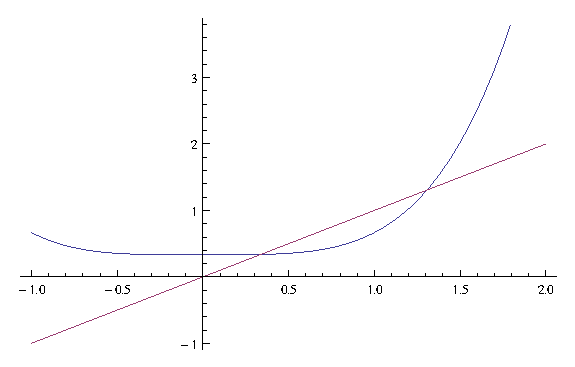
\includegraphics{Analysis/Analysis_sequence.eps}}
%\end{figure}

%\centertexdraw{
%
%    \def\bdot {\fcir f:0 r:0.03 }
%
%    \drawdim in
%
%    \arrowheadtype t:F \arrowheadsize l:0.08 w:0.04
%    \linewd 0.01 \setgray 0

%    \move (-1 -1) \lvec(2 2)
%    \move (-1 0) \clvec (1 0.5)(1.5 1)(2 1.5)
%
%    \move (-1 -1) \avec (-1 0 ) \avec(0 0) \avec(0 0.3) \avec(0.3 0.3) \avec(0.3 0.4)
%    \move (2 2) \avec (2 1.5) \avec(1.5 1.5) \avec(1.5 1.05) \avec(1.05 1.05) \avec(1.05 0.75) \avec(0.75 0.75) \avec(0.75 0.6)\avec(0.6 0.6)

%    \move (0.46 0.46) \bdot
%    \htext (-1.1 -1){0}
%    \htext (0.4 0.2){$r_1$}

%    \move (2 -1) \lvec(5 2)
%    \move (2.2 -1) \clvec (3.2 0.5)(3.4 1)(3.7 2)

%    \move (2.57 -0.43) \bdot
%    \move (3 0) \avec (3 0.3) \avec (3.3 0.3) \avec (3.3 0.85) \avec (3.85 0.85) \avec (3.85 2)
%    \htext (2.8 -0.5){$r_2$}

%\move (0 -1.2)
%}

Let the two roots of $f(x) = (x^4+1)/3 - x$ be $r_1$ and $r_2$ ($r_1 < r_2$). Because $f(0)>0$, $f(1) <0$ and $f(2) >0$, we have $r_1 \in (0,1)$ and $r_2\in (1,2)$.

Graphical analysis tells us that sequences starting with $a_1 =0,1$ converge to $r_1$ and $a_1 = 2$ diverges to infinity.

$a_1 = 0$. If $a_n \in (0,r_1)$, $f(a_n) = (a_n^4+1)/3 - a_n = a_{n+1} -a_n >0\ \ra \ a_{n+1} > a_n$. But
\be
a_{n+1} = (a_n^4+1)/3 < (r_1^4+1)/3 = r_1
\ee

Thus, $a_n$ is increasing and bounded above so it is converging.

$a_1 = 1$. If $a_n \in (r_1,r_2)$, $f(a_n) = (a_n^4+1)/3 - a_n = a_{n+1} -a_n < 0\ \ra \ a_{n+1} < a_n$. But
\be
a_{n+1} = (a_n^4+1)/3 > (r_1^4+1)/3 = r_1
\ee

Thus, $a_n$ is decreasing and bounded above so it is converging.

$a_1 = 2$. If $a_n \in (r_2,\infty)$, $f(a_n) = (a_n^4+1)/3 - a_n = a_{n+1} -a_n >0\ \ra \ a_{n+1} > a_n$. Thus, $a_n$ is increasing and unbounded above so it is diverging.
\end{solution}

%------------------------------------------------------------------------------------------------------------------

\begin{problem}
Let $a_1>b_1>0$ and let $a_{n+1} = (a_n + b_n)/2$, $b_{n+1} = 2a_nb_n/(a_n+b_n)$ for $n\geq 1$. Show that $a_n>a_{n+1}>b_{n+1}>b_n$ and deduce the two sequences converge to a common limit. What limit?
\end{problem}

\begin{solution}[\bf Solution.]
Since $a_1>b_1>0$,
\be
\left\{\ba{l}
2a_1 > a_1 + b_1 \ \ra \ a_1 > \frac{a_1 + b_1}2 = a_2\\
\frac 1{a_1} < \frac 1{b_1} \ \ra \  \frac 1{a_1} + \frac 1{b_1}  < \frac 2{b_1} \ \ra \ b_1 < \frac 2{\frac 1{a_1} + \frac 1{b_1}} = b_2\\
a_2 - b_2 = \frac{a_1 + b_1}2 - \frac {2a_1b_1}{a_1 + b_1} = \frac {(a_1 - b_1)^2}{2(a_1+b_1)} >0
\ea\right. \ \ra \ a_1 > a_2 > b_2 > b_1.
\ee

By induction, we have $a_n>a_{n+1}>b_{n+1}>b_n$. Since $a_n$ is a decreasing sequence, and bounded below (by 0), thus $a_n$ converges to $a$. Similarly, $b_n$ is an increasing sequence and bounded above (by $a_1$). Thus,
\be
\left\{\ba{l}
a = \frac {a+b}2 \\
b = \frac {2ab}{a+b}
\ea\right. \ \ra \ a = b.
\ee
which means that $a_n$ and $b_n$ converge to a common limit $c$. We know that
\be
a_{n+1}b_{n+1} = (a_n + b_n)/2 \times 2a_nb_n/(a_n+b_n) = a_n b_n \ \ra \ c^2 = a_1 b_1 \ \ra \ c = \sqrt{a_1b_1}.
\ee
\end{solution}

\subsection{Real series}

\begin{problem}[Baby Rudin Exercise 3.11]
Let $(a_n)_n$ be a positive real sequence. Suppose $s_n = a_1+\dots + a_n$ and $\sum_n a_n$ diverges. Prove that
\be
\frac{a_n}{s_n^2} \leq \frac 1{s_{n-1}} - \frac 1{s_n}
\ee
and deduce that $\sum_n \frac{a_n}{s_n^2}$ converges.

What can be said about
\be
\sum_n \frac {a_n}{1 + na_n}\quad \text{ and }\quad \sum_n \frac {a_n}{1 + n^2a_n}?
\ee
\end{problem}

\begin{solution}[\bf Solution.]
Clearly, for any $n\geq 2$,
\be
\frac 1{s_{n-1}} - \frac 1{s_n} = \frac {s_n - s_{n-1}}{s_{n-1}s_n} = \frac{a_n}{s_{n-1}s_n} \geq \frac{a_n}{s_n^2}
\ee

Thus, series $\frac 1{s_{n-1}} - \frac 1{s_n}$ is telescoping and
\be
\sum^\infty_{n=1} \frac{a_n}{s_n^2} \leq \frac 1{a_1} + \sum^\infty_{n=2} \frac 1{s_{n-1}} - \frac 1{s_n} = \frac 1{a_1} +  \frac 1{s_{1}} - \frac 1{s_\infty} = \frac 2{a_1}
\ee
as $s_\infty = \infty$. Thus, $\sum_n \frac{a_n}{s_n^2}$ converges as it is increasing and bounded.

Note that if $a_n=1/n$, $\sum_n \frac {a_n}{1 + na_n}$ diverges and $\sum_n \frac {a_n}{1 + n^2a_n}$ converges. Since the harmonic series is kind of a borderline divergent series, this suggests that the first series might always diverge and the second always converge.

However, if we let
\be
a_n = \begin{cases}
n=k! \quad\quad & \text{for some }k\in \Z^+,\\
2^{-n} & \text{otherwise.}
\end{cases}
\ee

The first case of that definition ensures that $\sum_n a_n$ diverges. Now we have
\be
\frac{a_n}{1 + na_n} = \frac{1}{n+\frac{1}{a_n}} =
\begin{cases}
\frac 1{n+1/n}\quad\quad & \text{if $n=k!$ for some }k\in \Z^+, \\
\frac 1{n+2^n} & \text{otherwise.}
\end{cases}
\ee

$\sum_n \frac 1{n+2^n}$ is certainly convergent, and
\be
\sum_{n=1}^\infty \frac 1{n!+1/n!} \leq \sum_{n=1}^\infty \frac 1{n!} = e.
\ee

So in this case $\sum_n \frac {a_n}{1 + na_n}$ converges. Thus, we cannot in general say anything about $\sum_n \frac {a_n}{1 + na_n}$.

For $\sum_n \frac {a_n}{1 + n^2a_n}$, on the other hand, succumbs to the comparison test:
\be
\frac{a_n}{1 + n^2a_n} = \frac 1{a_n^{-1} + n^2} < \frac 1{n^2} \ \ra\ \sum_n \frac {a_n}{1 + n^2a_n}\text{ converges.}
\ee
\end{solution}





\subsection{Differentiation}


\begin{problem}
Consider two contants $e^\pi$ and $\pi^e$. Which is bigger?
\end{problem}

\begin{solution}[\bf Solution.]
Consider the function
\be
f(x) = e^x - x^e,\qquad x\in \R
\ee
whose derivative is
\be
f'(x) = e^x - e \cdot x^{e-1}.
\ee

Note that exponential function and power function can have at most two points of intersection.\footnote{This is obvious by taking logarithm.} Therefore, $f'(x) =0$ implies $e^x = e \cdot x^{e-1}$ and we can find two points to satisfy this condition,
\be
f'(1) = e^1 - e\cdot 1^{e-1} = 0,\qquad f'(e) = e^e - e\cdot e^{e-1} = 0.
\ee

In general, an exponential function will grow to infinity faster than a power function\footnote{Again, taking logarithm will show the result.}, so
\be
f'(x) \geq 0,\quad x>e.
\ee

This means that $f$ is an increasing function when $x>e$. Also, notice that $f(e) =0$. Therefore, $f(\pi)>0$ since $f$ is increasing when $x>e$ and $\pi>e$.

Hence, $e^\pi > \pi^e$. Indeed, $e^\pi \approx 23.14$ and $\pi^e \approx 22.46$.
\end{solution}


\subsection{Monotone functions}


\begin{problem}
Given $f(x) = \log(x^2 -ax -1)$ is increasing when $x\in (1,+\infty)$. Find the range of $a$.
\end{problem}

\begin{solution}[\bf Solution.]
Since $\log$ is strictly increasing, we have that $x^2 - ax -1$ is increasing when $x\in (1,+\infty)$. As we know $x^2 -ax -1$ should have the U-shaped curve with symmetric axis at $x=a/2$.

\begin{center}
\psset{yunit=2.5cm,xunit=2.5cm}
\begin{pspicture}[algebraic](-0.5,-0.5)(2.5,2)%[showgrid](-3,-1.5)(3,4)
\psaxes[ticks=none,labels=none]{->}(0,0)(-0.5,-0.5)(2.5,2)%Dx=0.5,Dy=0.5
\psplot[linecolor=blue,linewidth=1.5pt]{-0.5}{2.5}{x^2-2*x+0.7}
\psline[linecolor=red,linestyle=dashed](1,2)(1,-0.5)
\rput(0.7,1.2){$x = a/2$}

\end{pspicture}
\end{center}

So $a/2$ must be smaller than 1 such that $x^2 - ax -1$ is increasing when $x\in (1,+\infty)$ which implies that
\be
a/2 \leq 1 \ \ra \ a\in (-\infty,2].
\ee
\end{solution}

\begin{problem}
Given $f(x) = (x-m)^{1/2}$ and its inverse function have common point. Find the range of $m$.
\end{problem}

\begin{solution}[\bf Solution.]
If $f(x)$ has common point with its inverse function, it must be on the line $y=x$ (since $f(x)$ and $f^{-1}(x)$ are symmetric about line $y=x$).


\begin{center}
\psset{yunit=2.5cm,xunit=2.5cm}
\begin{pspicture}[algebraic](-1,-0.75)(2.5,2)%[showgrid](-3,-1.5)(3,4)
\psaxes[ticks=none,labels=none]{->}(0,0)(-1,-0.75)(2.5,2)%Dx=0.5,Dy=0.5
\psplot[linecolor=blue,linewidth=1.5pt]{-0.5}{2.5}{(x+0.5)^0.5}
\psplot[linecolor=red,linewidth=1.5pt]{0}{1.6}{x^2-0.5}
\psline[linecolor=green,linestyle=dashed](-0.5,-0.5)(2,2)
%\psline[linecolor=red,linestyle=dashed](1,2)(1,-0.5)
\rput(2,1.9){$y=x$}
\rput(0.5,1.2){$f(x)$}
\rput(1.3,0.5){$f^{-1}(x)$}
\rput(-0.5,-0.1){$m$}
\end{pspicture}
\end{center}

So the extreme case is that $f(x)$ and $y=x$ only have one common point which implies that
\be
\begin{cases}
f'(x) - x' = 0 \quad \text{($f(x)-x$ achieves local maximum)}\\
f(x) -x = 0\quad \text{($f(x)$ is tangent to $y=x$)}
\end{cases} \ \ra\ \begin{cases}
(x-m)^{1/2} -x = 0 \\
\frac 12(x-m)^{-1/2} -1 = 0
\end{cases} \ \ra\ \begin{cases}
(x-m)^{1/2} = \frac 12 \\
(x-m)^{1/2} = x
\end{cases}
\ee

Thus, $x = \frac 12$ and $m = \frac 14$ which implies that the range should be $m \in (-\infty,\frac 14]$.
\end{solution}
